
%----------
%	CONFIGURACIÓN DEL DOCUMENTO
%----------

\documentclass[12pt]{report} %fuente a 12pt

% MÁRGENES: 2,5 cm sup. e inf.; 3 cm izdo. y dcho.
\usepackage[
a4paper,
vmargin=2.5cm,
hmargin=3cm
]{geometry}

\usepackage{booktabs}
\usepackage{amsmath}
\usepackage{longtable}

% INTERLINEADO: Estrecho (6 ptos./interlineado 1,15) o Moderado (6 ptos./interlineado 1,5)
\renewcommand{\baselinestretch}{1.15}
\parskip=6pt

% DEFINICIÓN DE COLORES para portada y listados de código
\usepackage[table]{xcolor}
\definecolor{azulUC3M}{RGB}{0,0,102}
\definecolor{gray97}{gray}{.97}
\definecolor{gray75}{gray}{.75}
\definecolor{gray45}{gray}{.45}

% Soporte para GENERAR PDF/A
\usepackage[a-1b]{pdfx}

% ENLACES
\usepackage{hyperref}
\hypersetup{colorlinks=true,
	linkcolor=black, % enlaces a partes del documento (p.e. índice) en color negro
	urlcolor=blue} % enlaces a recursos fuera del documento en azul

% EXPRESIONES MATEMATICAS
\usepackage{amsmath,amssymb,amsfonts,amsthm}

\usepackage{txfonts}
\usepackage[T1]{fontenc}
\usepackage{eurosym} % símbolo del euro (\euro) para el presupuesto
\usepackage[utf8]{inputenc}

\usepackage[spanish, es-tabla]{babel}
\usepackage[babel, spanish=spanish]{csquotes}
\AtBeginEnvironment{quote}{\small}

% diseño de PIE DE PÁGINA
\usepackage{fancyhdr}
\pagestyle{fancy}
\fancyhf{}
\renewcommand{\headrulewidth}{0pt}
\rfoot{\thepage}
\fancypagestyle{plain}{\pagestyle{fancy}}

% DISEÑO DE LOS TÍTULOS de las partes del trabajo (capítulos y epígrafes o subcapítulos)
\usepackage{titlesec}
\usepackage{titletoc}
\titleformat{\chapter}[block]
{\large\bfseries\filcenter}
{\thechapter.}
{5pt}
{\MakeUppercase}
{}
\titlespacing{\chapter}{0pt}{0pt}{*3}
\titlecontents{chapter}
[0pt]
{}
{\contentsmargin{0pt}\thecontentslabel.\enspace\uppercase}
{\contentsmargin{0pt}\uppercase}
{\titlerule*[.7pc]{.}\contentspage}

\titleformat{\section}
{\bfseries}
{\thesection.}
{5pt}
{}
\titlecontents{section}
[5pt]
{}
{\contentsmargin{0pt}\thecontentslabel.\enspace}
{\contentsmargin{0pt}}
{\titlerule*[.7pc]{.}\contentspage}

\titleformat{\subsection}
{\normalsize\bfseries}
{\thesubsection.}
{5pt}
{}
\titlecontents{subsection}
[10pt]
{}
{\contentsmargin{0pt}
	\thecontentslabel.\enspace}
{\contentsmargin{0pt}}
{\titlerule*[.7pc]{.}\contentspage}


% DISEÑO DE TABLAS. Puedes elegir entre el estilo para ingeniería o para ciencias sociales y humanidades. Por defecto, está activado el estilo de ingeniería.
\usepackage{multirow} % permite combinar celdas
\usepackage{caption} % para personalizar el título de tablas y figuras
\usepackage{floatrow} % utilizamos este paquete y sus macros \ttabbox y \ffigbox para alinear los nombres de tablas y figuras de acuerdo con el estilo definido
\usepackage{array} % con este paquete definimos un nuevo tipo de columna: ancho personalizado y contenido centrado
\newcolumntype{P}[1]{>{\centering\arraybackslash}p{#1}}
\DeclareCaptionFormat{upper}{#1#2\uppercase{#3}\par}

% Diseño de tabla para ingeniería
\captionsetup[table]{
	format=upper,
	name=TABLA,
	justification=centering,
	labelsep=period,
	width=.75\linewidth,
	labelfont=footnotesize,
	font=footnotesize,
}

%Diseño de tabla para ciencias sociales y humanidades
%\captionsetup[table]{
%	justification=raggedright,
%	labelsep=period,
%	labelfont=small,
%	singlelinecheck=false,
%	font={small,bf}
%}


% DISEÑO DE FIGURAS. Estilo de ingeniería activado por defecto.
\usepackage{graphicx}
\graphicspath{{imagenes/}{figuras/}} %rutas a las carpetas de imágenes y figuras

% Diseño de figuras para ingeniería
\captionsetup[figure]{
	format=hang,
	name=Fig.,
	singlelinecheck=off,
	labelsep=period,
	labelfont=footnotesize,
	font=footnotesize
}



% NOTAS A PIE DE PÁGINA
\usepackage{chngcntr} %para numeración contínua de las notas al pie
\counterwithout{footnote}{chapter}

% LISTADOS DE CÓDIGO
\usepackage{listings}
\usepackage{pdflscape} % páginas en horizontal (anexo de matrices anchas)

\lstdefinestyle{estilo}{ frame=Ltb,
	framerule=0pt,
	aboveskip=0.5cm,
	framextopmargin=3pt,
	framexbottommargin=3pt,
	framexleftmargin=0.4cm,
	framesep=0pt,
	rulesep=.4pt,
	backgroundcolor=\color{gray97},
	rulesepcolor=\color{black},
	%
	basicstyle=\ttfamily\footnotesize,
	keywordstyle=\bfseries,
	stringstyle=\ttfamily,
	showstringspaces = false,
	commentstyle=\color{gray45},
	%
	numbers=left,
	numbersep=15pt,
	numberstyle=\tiny,
	numberfirstline = false,
	breaklines=true,
	xleftmargin=\parindent
}

\captionsetup[lstlisting]{font=small, labelsep=period}
\lstset{style=estilo}
\lstdefinelanguage{Julia}{
	morekeywords={function,end,for,in,if,else,return,using,import,module,
		const,struct,mutable,where,do,begin,let,global,local},
	sensitive=true,
	morecomment=[l]{\#},
	morestring=[b]",
}

\lstset{
	extendedchars=true,
	literate={ξ}{{$\xi$}}1 {η}{{$\eta$}}1 {ζ}{{$\zeta$}}1
	{ε}{{$\varepsilon$}}1 {μ}{{$\mu$}}1 {∇}{{$\nabla$}}1
	{×}{{$\times$}}1 {á}{{\'a}}1 {é}{{\'e}}1 {í}{{\'i}}1
	{ó}{{\'o}}1 {ú}{{\'u}}1 {ñ}{{\~n}}1
	{₁}{{$_1$}}1 {₂}{{$_2$}}1 {→}{{$\rightarrow$}}1 {≤}{{$\leq$}}1
	{∈}{{$\in$}}1
	{₀}{{$_0$}}1 {₃}{{$_3$}}1 {ς}{{$\varsigma$}}1
	{‖}{{$\|$}}1 {ᵉ}{{$^e$}}1 {—}{{---}}1
	{⁴}{{$^4$}}1 {²}{{$^2$}}1 {−}{{$-$}}1
	{┌}{{>}}1 {└}{{>}}1
}
\renewcommand{\lstlistingname}{\uppercase{Código}}


%BIBLIOGRAFÍA

% CONFIGURACIÓN PARA LA BIBLIOGRAFÍA IEEE
\usepackage[backend=biber, style=ieee, isbn=false,sortcites, maxbibnames=5, minbibnames=1]{biblatex}

%CONFIGURACIÓN PARA LA BIBLIOGRAFÍA APA
%\usepackage[style=apa, backend=biber, natbib=true, hyperref=true, uniquelist=false, sortcites]{biblatex}
%\DeclareLanguageMapping{spanish}{spanish-apa}

\DefineBibliographyStrings{spanish}{%
	andothers = {et\addabbrvspace al\adddot}
}
\DefineBibliographyStrings{spanish}{
	url = {\adddot\space[En línea]\adddot\space Disponible en:}
}
\DefineBibliographyStrings{spanish}{
	urlseen = {Acceso:}
}
\DefineBibliographyStrings{spanish}{
	pages = {pp\adddot},
	page = {p.\adddot}
}

\addbibresource{bibliografia/bibliografia.bib} % archivo .bib con la bibliografía utilizada

% Atajo para las páginas de cortesía (en blanco) que exige la guía
\newcommand{\paginacortesia}{%
	\newpage
	\thispagestyle{empty}
	\mbox{}
}


%-------------
%	DOCUMENTO
%-------------

\begin{document}
\pagenumbering{roman} % cifras romanas en las páginas previas al cuerpo del trabajo

%==========================================================================
%	PORTADA (pág. I)
%==========================================================================
\begin{titlepage}
	\begin{sffamily}
	\color{azulUC3M}
	\begin{center}
		\begin{figure}[H] %incluimos el logotipo de la Universidad
			\makebox[\textwidth][c]{
\includegraphics[width=16cm]{Portada_Logo.png}}
		\end{figure}
		\vspace{2.5cm}
		\begin{Large}
			Grado Universitario en Ingeniería en Tecnologías de la Telecomunicación\\
			Curso académico 2025-2026\\
			\vspace{2cm}
			\textsl{Trabajo Fin de Grado}
			\bigskip

		\end{Large}
		 	{\Huge ``'Cálculo de Funciones de Base Hexaédricas de Elementos Finitos para Electromagnetismo en Julia''\par}
		 	\vspace*{0.5cm}
	 		\rule{10.5cm}{0.1mm}\\
			\vspace*{0.9cm}
			{\LARGE Antonio García Marugán}\\
			\vspace*{1cm}
			
		\begin{Large}
			Tutor/es\\
			Luis Emilio García Castillo\\
			Leganés, Septiembre de 2026\\
		\end{Large}
	\end{center}
	\vfill
	\color{black}
	
\includegraphics[width=4.2cm]{imagenes/creativecommons.png}\\
	Esta obra se encuentra sujeta a la licencia Creative Commons \textbf{Reconocimiento - No Comercial - Sin Obra Derivada}
	\end{sffamily}
\end{titlepage}

\paginacortesia % pág. II (en blanco)

%==========================================================================
%	RESUMEN Y PALABRAS CLAVE (pág. III)
%==========================================================================
\renewcommand\abstractname{\large\bfseries\filcenter\uppercase{Resumen}}
\begin{abstract}
\thispagestyle{plain}
\setcounter{page}{3}

	Este trabajo se centra en la implementación en Julia del elemento hexaédrico curl-conforme de Nédélec de segundo orden para el análisis mediante elementos finitos (FEM) en electromagnetismo computacional. Se emplea una formulación vectorial en el espacio $H(\mathrm{curl})$, para generar de forma sistemática las 54 funciones de base para construir un elemento de referencia y pasarlo al elemento real mediante la transformación de Piola, y se verifica el código frente a una implementación de referencia en MATLAB. Se verifica frente a los resultados del paper, el análisis de los autovalores de una cavidad semillena (inhomogénea) de material dieléctrico, la comparación de rendimiento y de eficiencia en memoria.

	\vspace{0.5cm}
	\textbf{Palabras clave:} Funciones de base curl-conformes; Análisis de elementos finitos; Hexaedros; Julia; N\'ed\'elec

	\vfill
\end{abstract}

\paginacortesia % pág. IV (en blanco)


%==========================================================================
%	DEDICATORIA / AGRADECIMIENTOS (pág. V)
%==========================================================================
\chapter*{Dedicatoria}
\setcounter{page}{5}

	% ESCRIBIR AQUÍ LA DEDICATORIA O LOS AGRADECIMIENTOS
	Se dice que la dedicatoria es la parte más leída de la mayoría de Trabajos de Fin de Grado. Aunque al principio cuando me enteré de ese dato me dio algo de pena. Conforme más vueltas le doy más me alegra que si alguien se tiene que enterar de algo de este trabajo sea de las personas que me han ayudado a llegar hasta aquí. Mis padres Pilar y Sebastián, mi hermana María Victoria, mis abuelos Pruden, Mari, Pedro y Antonio, y por último a quien más me ha soportado a mí y a este trabajo, Marina.
	
	También quiero agradecer a Luis por su casi infinita paciencia conmigo y por introducirme a Julia y al mundo de los elementos finitos.

	\vfill

\paginacortesia % pág. VI (en blanco)


%==========================================================================
%	ÍNDICES
%==========================================================================

\tableofcontents
\thispagestyle{fancy}

\paginacortesia

\listoffigures
\thispagestyle{fancy}

\paginacortesia

\listoftables
\thispagestyle{fancy}

\paginacortesia

\phantomsection
\chapter*{Lista de abreviaturas}
\addcontentsline{toc}{chapter}{Lista de abreviaturas}

\begin{tabbing}
	ABREV \quad\= Desarrollo completo de la abreviatura \kill
	API \> Application Programming Interface (interfaz de programación de aplicaciones) \\
	ARPACK \> Arnoldi Package (paquete de resolución de autovalores) \\
	BLAS \> Basic Linear Algebra Subprograms \\
	CC \> Creative Commons \\
	COO \> Coordinate list (lista de coordenadas; formato disperso de tripletes) \\
	CPU \> Central Processing Unit (unidad central de procesamiento) \\
	CSC \> Compressed Sparse Column (columnas comprimidas; formato disperso) \\
	DOF \> Degrees of Freedom (grados de libertad) \\
	ECTS \> European Credit Transfer and Accumulation System (sistema europeo de transferencia y acumulación de créditos) \\
	EPS \> Escuela Politécnica Superior \\
	FEM \> Finite Element Method (método de los elementos finitos) \\
	Gmsh \> Generador de mallas de elementos finitos \\
	GNU \> GNU's Not Unix (proyecto de software libre) \\
	GPL \> GNU General Public License (licencia pública general de GNU) \\
	GREMA \> Grupo de Radiofrecuencia, Electromagnetismo, Microondas y Antenas \\
	HOFEM \> Higher Order Finite Element Method \\
	IEEE \> Institute of Electrical and Electronics Engineers \\
	IR \> Intermediate Representation (representación intermedia) \\
	JIT \> Just-In-Time (compilación en tiempo de ejecución) \\
	LAPACK \> Linear Algebra Package (paquete de álgebra lineal) \\
	LLVM \> Low Level Virtual Machine (máquina virtual de bajo nivel) \\
	MIT \> Massachusetts Institute of Technology (licencia de software libre) \\
	PEC \> Perfect Electric Conductor (conductor eléctrico perfecto) \\
	POO \> Programación Orientada a Objetos \\
	RAM \> Random Access Memory (memoria de acceso aleatorio) \\
	REPL \> Read-Eval-Print Loop (bucle de lectura-evaluación-impresión) \\
	RGPD \> Reglamento General de Protección de Datos \\
	SMI \> Salario Mínimo Interprofesional \\
	TFG \> Trabajo de Fin de Grado \\
	UC3M \> Universidad Carlos III de Madrid
\end{tabbing}

\paginacortesia


%==========================================================================
%	CUERPO DEL TRABAJO (numeración arábiga a partir de aquí)
%==========================================================================
\clearpage
\pagenumbering{arabic}

%--------------------------------------------------------------------------
\chapter{Introducción}\label{cap:introduccion}
El electromagnetismo computacional y el análisis mediante elementos finitos (FEM por sus siglas en inglés) son herramientas fundamentales para obtener soluciones numéricas a problemas físicos complejos o sin soluciones analíticas. Uno de los pilares de FEM es la selección de funciones de base adecuadas que eviten la aparición de soluciones espurias, aseguran la continuidad tangencial y permiten la discontinuidad en la componente normal. Este trabajo se centra en la implementación en Julia de un conjunto concreto de esas funciones de base, el elemento hexaédrico curl-conforme de Nédélec de segundo orden
propuesto en \cite{amor2023hexahedral}, y verifica la implementación resolviendo el mismo problema de referencia (una cavidad semillena) frente a la implementación en MATLAB proporcionada en \cite{amor2022zenodo}
%--------------------------------------------------------------------------

\section{Motivación}\label{sec:motivacion}
El Grupo de Radiofrecuencia, Electromagnetismo, Microondas y Antenas
(GREMA) de la Universidad Carlos III de Madrid ha contribuido al electromagnetismo computacional con especial énfasis en FEM desarrollando herramientas como HOFEM (\emph{Higher Order
Finite Element Method}) \cite{garciadonoro2015hofem}. HOFEM discretiza
la ecuación de onda vectorial de doble rotacional mediante tetraedros y prismas
curl-conformes isoparamétricos de la primera familia de N\'ed\'elec y se puede utilizar mediante un simulador gráfico tanto en Linux como en Windows.

El simulador está escrito en Fortran y hace uso de ciertos elementos de la programación orientada a objetos con el objetivo de hacerlo mantenible. Sin embargo, en muchas ocasiones en la programación científica se utiliza un lenguaje de alto nivel (MATLAB o Python) que permita realizar un prototipo o prueba de concepto y luego utilizar las funcionalidades de Fortran, como la alta eficiencia, la portabilidad o la capacidad de programación en paralelo, para crear el producto definitivo.

Con el objetivo de acercar ambas aproximaciones y rebajar esa barrera de
entrada, sin sacrificar el rendimiento, se planteó implementar
progresivamente en Julia distintas funcionalidades de HOFEM. Entre las
características del lenguaje que lo hacen adecuado para este propósito
\cite{bezanson2017julia} cabe destacar:

\begin{itemize}
	\item La inferencia de tipos, que permite declararlos o no sin sacrificar 
	en rendimiento, ya que el compilador es capaz de hacerlo del tipo con el que se llama a la función.
	\item El \emph{multiple dispatch}, que selecciona la implementación de una
	función en función de los tipos de todos sus argumentos, de modo que una
	misma rutina sirve tanto para reales como complejos
	\item la utilización de caracteres Unicode que permite mejorar la legibilidad del código como se ve en ~\ref{cod:jacobiano}.
	\item No hace falta vectorizar para aumentar el rendimiento.
	\item Los tipos definidos por el usuario tienen una eficiencia parecida a los del propio lenguaje.
\end{itemize}
\begin{lstlisting}[language=Julia, caption={Construcción de la matriz jacobiana del mapeo isoparamétrico.}, label=cod:jacobiano]
	function compute_jacobian(nodes, pt)
	ξ, η, ζ = pt
	dNdξ = [-(1-η)*(1-ζ), (1-η)*(1-ζ), η*(1-ζ), -η*(1-ζ),
	-(1-η)*ζ,     (1-η)*ζ,     η*ζ,     -η*ζ]
	...
\end{lstlisting}

Teniendo en cuenta ese contexto, este Trabajo de Fin de Grado implementa en Julia el elemento hexaédrico curl-conforme de N\'ed\'elec de segundo orden propuesto en \cite{amor2023hexahedral}. La implementación se verifica comprobando que pase una serie de tests que se construyen unos encima de otros y se contrasta (en rendimiento y en resultados) con la implementación de \cite{amor2022zenodo}, que utiliza MATLAB con POO (Programación Orientada a Objetos), una aproximación diferente a la utilizada aquí.

\section{Objetivos}\label{sec:objetivos}
El objetivo general de este trabajo es implementar en Julia las funciones de
base del elemento hexaédrico curl-conforme de N\'ed\'elec de segundo orden
propuesto en \cite{amor2023hexahedral} y verificar su correcto funcionamiento
resolviendo, con ellas, el mismo problema de referencia que la implementación
en MATLAB de \cite{amor2022zenodo}. Para alcanzar este objetivo general se
plantean los siguientes objetivos específicos, que cubren tanto la
construcción de las funciones de base como su validación por niveles
crecientes de complejidad:
\begin{itemize}
	\item O1. Implementar en Julia las funciones de base del elemento hexaédrico curl-conforme de Nédélec de segundo orden y los módulos necesarios para evaluarlas, ensamblarlas y compararlas con una solución analítica.
	\item O2. Obtener los coeficientes de las funciones de base y comprobar que reproducen los resultados de la Tabla II del artículo.
	\item O3. Verificar el ensamblaje global comprobando que las matrices $\mathbf{K}$ y $\mathbf{M}$ tienen la dimensión del núcleo correcta y coinciden con las de la implementación MATLAB existente.
	\item O4. Reproducir el benchmark de la cavidad semillena y su convergencia, comprobando que los autovalores coinciden con la solución analítica y con MATLAB, y que el marco implementado admite distintas mallas y topologías.
	\item O5. Comparar el rendimiento de ambas implementaciones.
\end{itemize}

\section{Estructura del documento}\label{sec:estructura}
La memoria está compuesta de los siguientes capítulos. En el primer capítulo Introducción se expone la motivación detrás del desarrollo del trabajo y los objetivos a completar con este. En el siguiente capítulo Estado del Arte se presenta el marco teórico utilizado en la realización de la implementación que incluye: ecuaciones de Maxwell y como se deriva la ecuación de onda de Helmholtz, las condiciones de contorno del problema, como se plantea el problema de autovalores, el método de los elementos finitos en electromagnetismo, el espacio $H(\mathrm{curl})$ y la aparición de modos espurios que explica el uso de elementos de Nédélec.

El capítulo Métodos detalla paso por paso la implementación en Julia. Es una explicación secuencial en la que cada paso se construye sobre el anterior. Incluye la implementación de: el elemento de referencia, el espacio $\mathcal{H}_2$ y sus monomios, los grados de libertad de arista, cara y volumen, la generación de los coeficientes de las funciones de base, su evaluación en el elemento real, el mallado y etiquetado, el ensamblaje del sistema, la resolución del problema de autovalores y la arquitectura del paquete \texttt{NedelecHex}.

El capítulo \emph{Resultados} expone los resultados obtenidos y los valida frente a los resultados del paper y la implementación de MATLAB. En el capítulo Discusión de los resultados y conclusiones se identifican las limitaciones del trabajo y las líneas futuras en las que se podría expandir la el paquete de código.

Por último, los capítulos \emph{Marco regulador} y \emph{Entorno socio-económico} presentan la normativa relevante y la actividad socio-económica derivada del Trabajo de Fin de Grado, mientras que los anexos aportan información complementaria. El Anexo A es la salida completa de los tests realizados, el Anexo B la salida sin redondear de los coeficientes de ambos lenguajes y el Anexo C la declaración de uso de la IA generativa.
%--------------------------------------------------------------------------
\chapter{Estado del arte}\label{cap:estado-arte}
%--------------------------------------------------------------------------

\section {Ecuaciones de Maxwell}\label{subsec:maxwell-t}
En el dominio de la frecuencia y para un medio lineal e isótropo, las
ecuaciones de Maxwell pueden escribirse en forma fasorial como
\cite{jin2015, jacobsson2007nedelec}:
\begin{align}
	\nabla \times \mathbf{E} &= -j\omega\mu\mathbf{H}, \qquad \text{(ley de Faraday)} \label{eq:maxwell-faraday}\\
	\nabla \times \mathbf{H} &= j\omega\varepsilon\mathbf{E} + \mathbf{J}, \qquad \text{(ley de Amp\`ere--Maxwell)} \label{eq:maxwell-ampere}\\
	\nabla \cdot (\varepsilon\mathbf{E}) &= \rho, \qquad \text{(ley de Gauss)} \label{eq:maxwell-gauss}\\
	\nabla \cdot (\mu\mathbf{H}) &= 0, \qquad \text{(ley de Gauss magn\'etica)} \label{eq:maxwell-gauss-mag}\\
	\nabla \cdot \mathbf{J} &= -j\omega\rho. \qquad \text{(ecuaci\'on de continuidad)} \label{eq:maxwell-continuidad}
\end{align}
De las cinco ecuaciones solo tres son independientes: basta con
\eqref{eq:maxwell-faraday}, \eqref{eq:maxwell-ampere} y \eqref{eq:maxwell-gauss},
o bien con \eqref{eq:maxwell-faraday}, \eqref{eq:maxwell-ampere} y
\eqref{eq:maxwell-continuidad}. 

\subsection{Ecuaci\'on de onda de Helmholtz}\label{subsec:maxwell-f}
En ausencia de fuentes ($\mathbf{J}=\mathbf{0}$, $\rho=0$) y para un medio
lineal e is\'otropo, las ecuaciones \eqref{eq:maxwell-faraday} y
\eqref{eq:maxwell-ampere} se reducen a \cite{jin2015, pozar2012}:
\begin{align}
	\nabla \times \mathbf{E} &= -j\omega\mu_0\mu_r\, \mathbf{H}, \label{eq:faraday}\\
	\nabla \times \mathbf{H} &= j\omega\varepsilon_0\varepsilon_r\, \mathbf{E}. \label{eq:ampere}
\end{align}
Aplicando el rotacional a \eqref{eq:faraday} y sustituyendo en
\eqref{eq:ampere} \cite{jin2015, jacobsson2007nedelec}:
\begin{align}
	\nabla \times (\nabla \times \mathbf{E})
	&= -j\omega\mu_0\mu_r\, \nabla \times \mathbf{H}
	= -j\omega\mu_0\mu_r\, (j\omega\varepsilon_0\varepsilon_r \mathbf{E})
	\nonumber\\
	&= \omega^2\mu_0\varepsilon_0\, \mu_r\varepsilon_r \mathbf{E}.
\end{align}
Dividiendo entre $\mu_r$ y con $k_0^2 = \omega^2\mu_0\varepsilon_0$:
\begin{equation}\label{eq:curlcurl}
	\nabla \times \left( \frac{1}{\mu_r} \nabla \times \mathbf{E} \right)
	- k_0^2\, \varepsilon_r\, \mathbf{E} = \mathbf{0}
	\qquad \text{en } \Omega.
\end{equation}
Esta es la ecuaci\'on de onda de Helmholtz, que es lo que se busca resolver en
gu\'ias de onda y cavidades, una vez aplicadas las condiciones de contorno del
problema.

\section{Condiciones de contorno}\label{subsec:pec}
Para describir correctamente un problema de electromagnetismo se deben incluir tanto las ecuaciones diferenciales como las condiciones de contorno \cite{jin2015}.

\subsubsection{Continuidad entre dos medios}
En una interfaz sin fuentes entre dos medios, los campos deben satisfacer las
condiciones de continuidad
\begin{align}
	\hat{\mathbf{n}} \times (\mathbf{E}_1 - \mathbf{E}_2) &= \mathbf{0}, \label{eq:bc-et}\\
	\hat{\mathbf{n}} \cdot (\mathbf{B}_1 - \mathbf{B}_2) &= 0, \label{eq:bc-bn}
\end{align}
donde $\hat{\mathbf{n}}$ es el vector normal unitario a la interfaz. De estas
dos condiciones, la primera expresa la continuidad de la componente tangencial
de $\mathbf{E}$ y la segunda la de la componente normal de $\mathbf{B}$.

\subsubsection{Conductores perfectos}
Cuando uno de los medios es un conductor perfecto (PEC), este no puede
sostener campos internos, por lo que las condiciones \eqref{eq:bc-et} y
\eqref{eq:bc-bn} se reducen a
\begin{equation}\label{eq:pec}
	\hat{\mathbf{n}} \times \mathbf{E} = \mathbf{0}
	\qquad \text{y} \qquad
	\hat{\mathbf{n}} \cdot \mathbf{B} = 0
	\qquad \text{en } \partial\Omega,
\end{equation}
donde $\mathbf{E}$ y $\mathbf{B}$ son los campos exteriores al conductor y
$\hat{\mathbf{n}}$ es la normal que apunta hacia fuera del conductor.

Cuando se impone el valor de la función incógnita sobre el contorno se conoce como imponer condiciones de Dirichlet, como en nuestro caso, el de una cavidad semillena rellena de una losa de dieléctrico y rodeada de un conductor perfecto. Los grados de libertad (DOFs)
asociados a las aristas y caras del contorno $\partial\Omega$ se fijan a cero
por lo que se cumple que $\hat{\mathbf{n}}\times\mathbf{E}=\mathbf{0}$ sobre la frontera.


\begin{figure}[H]
	\ffigbox[\FBwidth]
	{\caption[Cavidad semillena rellena hasta $y=b/2$ de una losa de material diel\'ectrico y el resto de vac\'io, cubierta por un conductor perfecto (PEC)]{Cavidad semillena rellena hasta $y=b/2$ de una losa de material diel\'ectrico y el resto de vac\'io, cubierta por un conductor perfecto (PEC).}\label{fig:guia_onda_pec}}
	{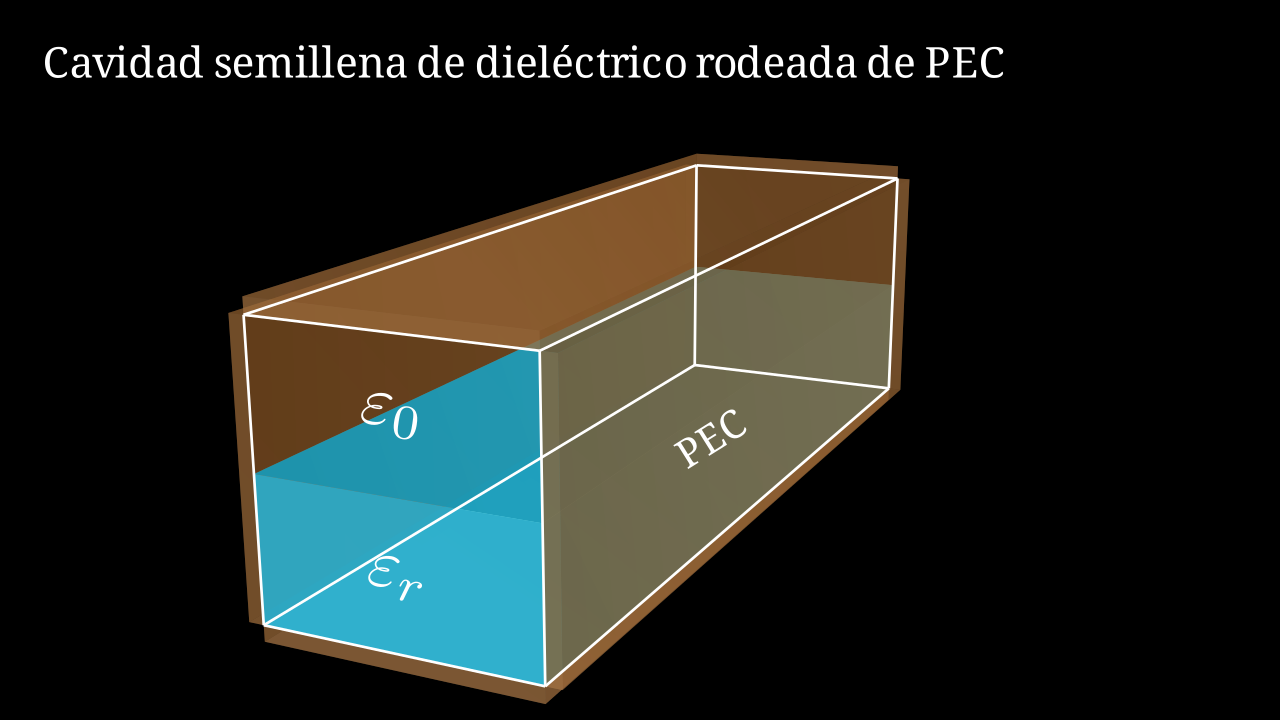
\includegraphics[width=0.85\linewidth]{guia_onda_pec.png}}
\end{figure}

\section{Problema de autovalores}\label{subsec:autovalores}
Un problema de autovalores se define de la siguiente manera:
Dada una matriz $\mathbf{A}$, un \emph{autovalor} $\lambda$ y su \emph{autovector}
$\mathbf{v}\neq\mathbf{0}$ cumplen que:
\begin{equation}\label{eq:autovalor-def}
	\mathbf{A}\,\mathbf{v} = \lambda\,\mathbf{v}.
\end{equation}
Dicho de otra manera, al aplicar $\mathbf{A}$ al autovector, el resultado es el mismo vector
multiplicado por un escalar. $\mathbf{A}$ solo lo alarga o lo encoge sin cambiar su direcci\'on, y el autovalor $\lambda$ es ese factor de escala.

Como $\mathbf{v}$ y $\lambda$ en general son ambos desconocidos lo que se busca son pares $(\lambda,\mathbf{v})$ que hacen que $\mathbf{A}\mathbf{v}-\lambda\mathbf{v}=\mathbf{0}$ tenga soluci\'on no trivial. En general hay tantas parejas como la
dimensi\'on del espacio. En nuestro caso:
\begin{equation}
	\nabla \times \left( \frac{1}{\mu_r} \nabla \times \mathbf{E} \right)
	- k_0^2\, \varepsilon_r\, \mathbf{E} = \mathbf{0}
	\qquad \text{en } \Omega.
\end{equation}

El operador es un operador diferencial ($\nabla\times\nabla\times$) pero el proceso es el mismo. Se buscan los campos $\mathbf{E}\neq\mathbf{0}$ y los
escalares $k_0^2$ tales que el operador aplicado al campo sea un m\'ultiplo
escalar del propio campo.

Resolver \eqref{eq:curlcurl} es un problema de autovalores. Se puede ver más claramente si lo escribimos como \eqref{eq:autovalor-def}:
\begin{equation}\label{eq:autovalor-continuo}
	\nabla \times \left( \frac{1}{\mu_r} \nabla \times \mathbf{E} \right)
	= k_0^2\, \varepsilon_r\, \mathbf{E}
	\qquad \text{en } \Omega,
	\qquad \hat{\mathbf{n}} \times \mathbf{E} = \mathbf{0}
	\quad \text{en } \partial\Omega .
\end{equation}
Se busca el conjunto de pares $(k_0^2, \mathbf{E})$ con
$\mathbf{E}\neq\mathbf{0}$ que satisfacen esta ecuación.
Estos autovalores corresponden a los modos de resonancia de la cavidad, que se
identifican mediante los \'indices $TE_{mn\ell}$ o
$TM_{mn\ell}$, donde $m$, $n$ y $\ell$ son el n\'umero de variaciones del
campo respectivo en cada direcci\'on. La relaci\'on entre el n\'umero de
onda de resonancia y la frecuencia de resonancia viene dada por
$k_0 = \omega\sqrt{\mu_0\varepsilon_0}$, por lo que con los autovalores se
pueden obtener las frecuencias de resonancia \cite{pozar2012}.

\section{El método de los elementos finitos en electromagnetismo}\label{sec:mef}
Para resolver el problema de autovalores que acabamos de plantear, que se basa en resolver una ecuación diferencial con unas ciertas condiciones de contorno, a menudo se utilizan técnicas numéricas como el método de los elementos finitos (FEM).

El objetivo de FEM es sustituir el dominio continuo $\Omega$ por un conjunto finito de subdominios más simples, los elementos, en los que la función incógnita se aproxima mediante funciones de interpolación (polinomios de un determinado orden) con coeficientes desconocidos. De este modo la solución en todo el dominio queda aproximada por un número finito de incógnitas y coeficientes. Según \cite{jin2015} el procedimiento se puede definir en cuatro etapas:

\subsection{Discretización del dominio}\label{subsec:mef-discretizacion}
Consiste en subdividir $\Omega$ en elementos con los que aproximar el dominio. Se describe más en detalle en el apartado de métodos en \autoref{sec:mallado} (generación y etiquetado con Gmsh, \autoref{sec:gmsh}).

En este trabajo nos centraremos en el caso tridimensional, en el que el dominio se subdivide en \emph{hexaedros}.

\subsection{Selección de las funciones de interpolación}\label{subsec:mef-interpolacion}
La definición que se utiliza en el paper de referencia \cite{amor2023hexahedral} es la propuesta por Ciarlet \cite{ciarlet2002}, donde un elemento finito queda definido por la terna:
\begin{equation}\label{eq:terna-ciarlet}
	(K,\, P_K,\, \Sigma_K),
\end{equation}
\begin{enumerate}
	\item \textbf{$K$ es un dominio geométrico simple} (por ejemplo un tetraedro, un hexaedro o un prisma; en nuestro caso, el hexaedro de referencia $H=[0,1]^3$).
	\item \textbf{$P_K$ es un espacio de funciones}, habitualmente polinomios, definidas sobre un espacio (en nuestro caso, $P_K=\mathcal{H}_2$, el espacio de 54 monomios definido en \eqref{eq:h2}).
	\item \textbf{$\Sigma_K$ es un conjunto de \emph{funcionales lineales}} aplicadas sobre $P_K$. Estos funcionales son lo que denominamos como  \emph{grados de libertad} (DOF, del inglés \emph{degrees of freedom}) del elemento finito.
\end{enumerate}

\subsection{Creación del sistema de ecuaciones}\label{subsec:mef-sistema}
Para pasar de la ecuaci\'on diferencial \eqref{eq:curlcurl} al sistema de ecuaciones se utiliza la \emph{formulaci\'on d\'ebil}, ya que la formulación débil relaja los requisitos de regularidad (basta con que la solución y su rotacional sean de cuadrado integrable) y permite trabajar en espacios de Hilbert donde se puede demostrar la convergencia del método.

El problema que queremos resolver, lo que se denomina como formulación fuerte, es la siguiente ecuación diferencial donde se busca encontrar el campo el\'ectrico $\mathbf{E}$ tal que:
\begin{equation}\label{eq:forma-fuerte}
	\nabla \times \left( \frac{1}{\mu_r} \nabla \times \mathbf{E} \right) - k_0^2\, \varepsilon_r\, \mathbf{E} = \mathbf{0}
	\qquad \text{en } \Omega,
\end{equation}

Como se ha mencionado anteriormente, es conveniente reescribir \eqref{eq:forma-fuerte} como una ecuación de forma integral. Esto se debe a que \eqref{eq:forma-fuerte} requiere que la solución sea diferenciable dos veces en todo el dominio, lo cual es un problema en FEM, ya que el dominio puede tener discontinuidades entre medios y las soluciones de FEM se aproximan con polinomios a trozos continuos cuyas derivadas no están bien definidas en las fronteras entre elementos.

\begin{figure}[H]
	\centering
	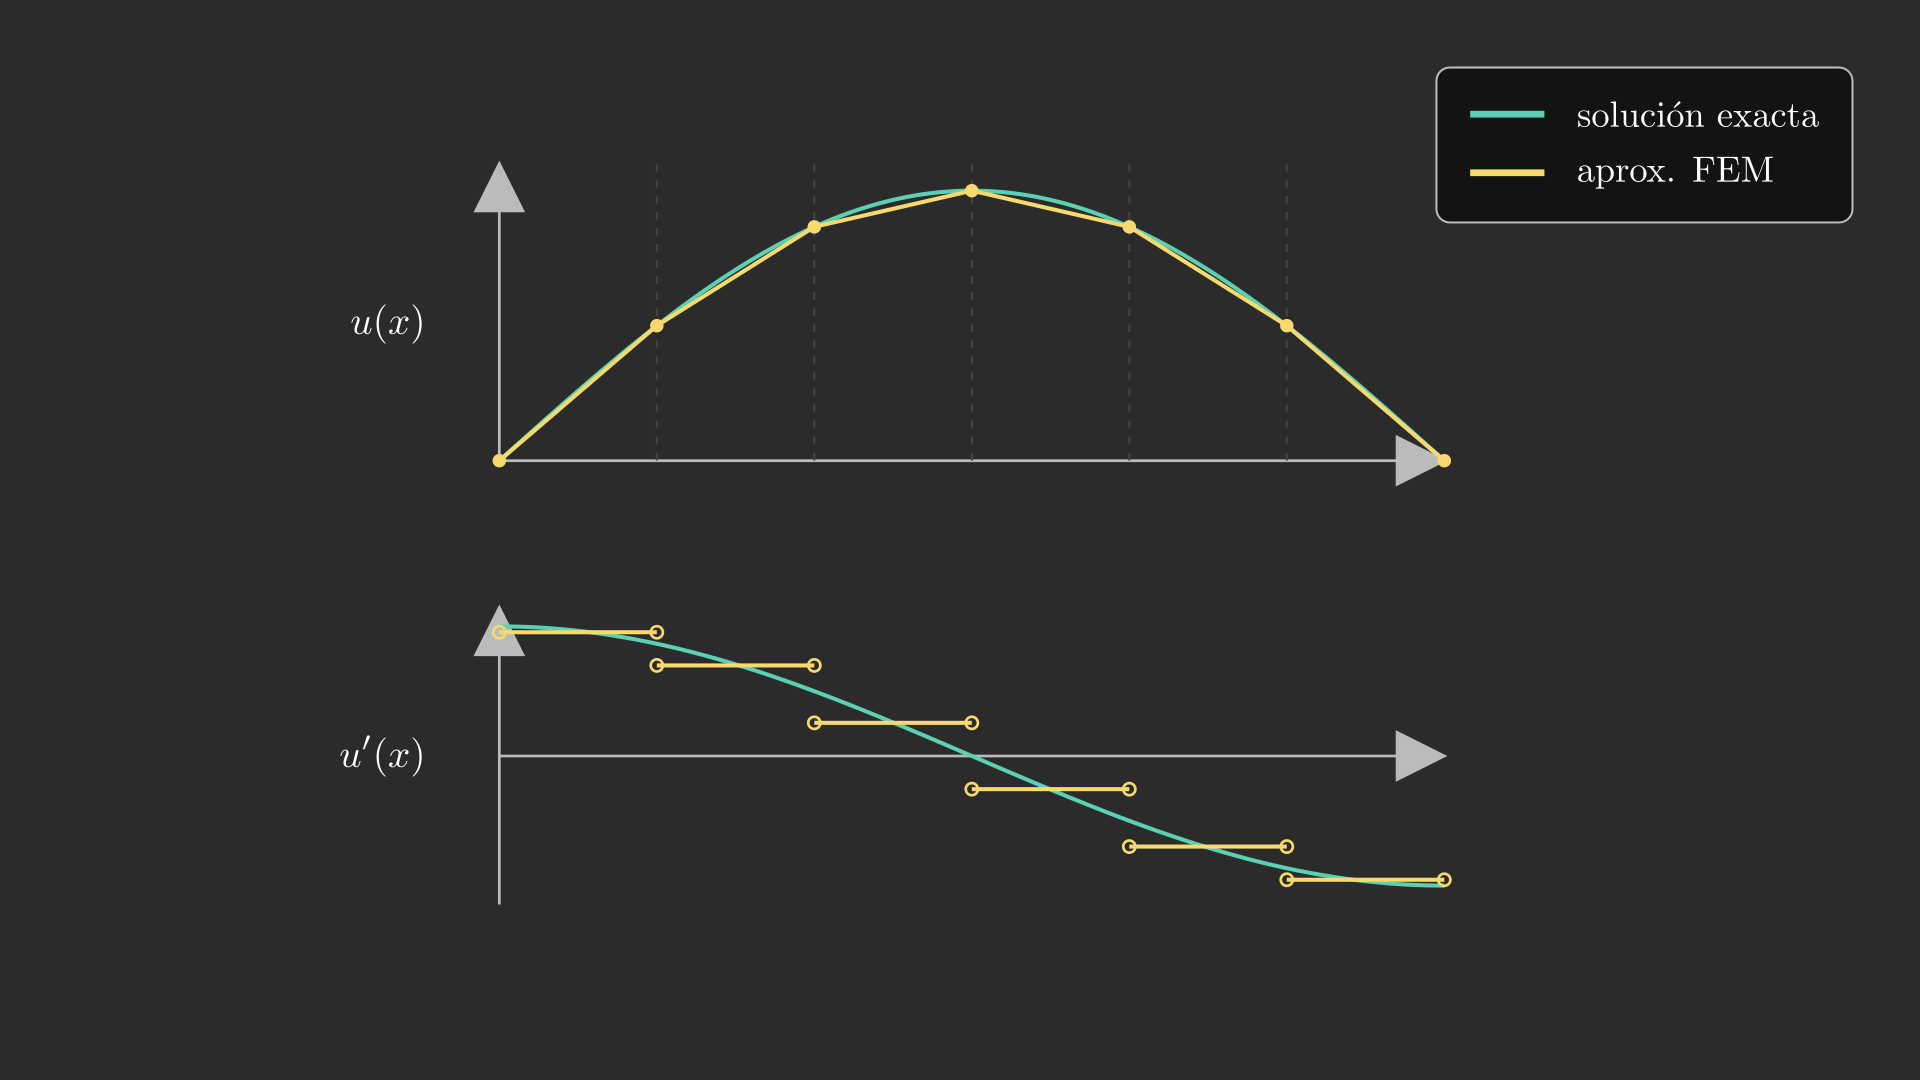
\includegraphics[width=0.85\linewidth]{regularidad.png}
	\caption[Problema de la formulación fuerte al diferenciar]{Al aproximar con polinomios a trozos continuos al diferenciar se producen discontinuidades.}\label{fig:regularidad}
\end{figure}

La formulación débil dice que en lugar de pedir que \eqref{eq:forma-fuerte} se cumpla en todos los puntos de  $\Omega$, se puede multiplicar la ecuaci\'on por una funci\'on arbitraria de prueba llamada $\mathbf{v}$ y se integra sobre el dominio de la función de prueba. Si la ecuaci\'on se cumple para todas las $\mathbf{v}$, entonces se cumple en todo el dominio \cite{liu2014weakform}. Se puede reescribir entonces \eqref{eq:forma-fuerte} como:

 Encuentra $\mathbf{E}$ tal que:
\begin{equation}\label{eq:forma-debil-fuerte}
	\int_\Omega \mathbf{v}\cdot\left[\nabla \times \left( \frac{1}{\mu_r} \nabla \times \mathbf{E} \right) - k_0^2 \varepsilon_r \mathbf{E} \right] d\Omega = 0
	\qquad \forall\,\mathbf{v},
\end{equation}
es decir, que el residuo de la ecuaci\'on sea ortogonal a todas las funciones de prueba.

Aplicando integraci\'on por partes y la condición de contorno de Dirichlet en el espacio $H_0(\mathrm{curl},\Omega)$ queda como:

\begin{equation}\label{eq:forma-debil-h0}
	\int_\Omega \frac{1}{\mu_r} (\nabla\times\mathbf{E})\cdot(\nabla\times\mathbf{v})\,d\Omega
	- k_0^2 \int_\Omega \varepsilon_r \mathbf{E}\cdot\mathbf{v}\,d\Omega = 0
	\qquad \forall\,\mathbf{v}\in H_0(\mathrm{curl},\Omega).
\end{equation}

Esta forma d\'ebil \eqref{eq:forma-debil-h0} es la que se discretiza con el m\'etodo de los elementos finitos: al restringir $\mathbf{E}$ y $\mathbf{v}$ al espacio de funciones de base, la integral se convierte en un sistema de ecuaciones lineales.

\subsection{Resolución del sistema de ecuaciones}\label{subsec:mef-resolucion}
La \'ultima etapa consiste en resolver num\'ericamente el sistema construido. En nuestro caso es un problema algebraico de autovalores generalizado, que se resuelve con un solucionador de autovalores (la rutina \texttt{eigs} de MATLAB o su equivalente en Julia), como se describe en el cap\'itulo de resultados.

\section{El espacio $H(\mathrm{curl})$}\label{sec:hcurl}
Para un dominio tridimensional $\Omega$, el espacio de funciones curl-conformes se define como \cite{amor2023hexahedral}
\begin{equation}\label{eq:hcurl}
	H(\mathrm{curl},\Omega) := \left\{ \mathbf{u} \in [L^2(\Omega)]^3 \;\middle|\; \nabla\times\mathbf{u} \in [L^2(\Omega)]^3 \right\},
\end{equation}
donde $L^2(\Omega)$ es el espacio de funciones de cuadrado integrable sobre $\Omega$, es decir, con energía finita, y cuyo rotacional también tiene energía finita.
Si lo juntamos con las condiciones de contorno:
\begin{equation}\label{eq:hcurl0}
	H_0(\mathrm{curl},\Omega) := \left\{ \mathbf{u} \in H(\mathrm{curl},\Omega) \;\middle|\; \hat{\mathbf{n}}\times\mathbf{u} = \mathbf{0} \text{ en } \partial\Omega_D \right\},
\end{equation}
donde $\hat{\mathbf{n}}$ es el vector normal unitario a $\partial\Omega_D$, el contorno de la cavidad sobre el cual se impone la condición de Dirichlet (campo nulo, ya que es un conductor perfecto).

La importancia de $H(\mathrm{curl},\Omega)$ viene de que es el espacio al que pertenece el campo eléctrico. En un cambio de medio entre dos dieléctricos se debe respetar continuidad en la componente tangencial
\begin{equation}\label{eq:continuidad-tangencial}
	\hat{\mathbf{n}} \times (\mathbf{E}_1 - \mathbf{E}_2) = \mathbf{0},
\end{equation}
Mientras que en ausencia de cargas libres la componente normal cumple:
	\begin{equation}\label{eq:continuidad-dn}
	\hat{\mathbf{n}} \cdot (\mathbf{D}_1 - \mathbf{D}_2) = 0
	\quad\Longrightarrow\quad
	\varepsilon_1 E_{n,1} = \varepsilon_2 E_{n,2},
\end{equation}

Por lo que si $\varepsilon_1\neq\varepsilon_2$ la componente normal $E_n$ cambia entre interfaces.

Es por lo explicado anteriormente que se elige $H(\mathrm{curl},\Omega)$. Matemáticamente es suficiente porque la formulación débil solo exige que E y su rotacional $\nabla\times\mathbf{E}$ sean cuadrado integrable lo cual se cumple en $H(\mathrm{curl},\Omega)$. Adicionalmente exige la continuidad de la componente tangencial y permite la discontinuidad de la componente normal las cuales son propiedades del campo eléctrico que buscamos encontrar numéricamente. Imponer estas propiedades a los elementos finitos nos lleva a implementar elementos de arista de Nédélec como se expone a continuación.

\section{Modos espurios y elementos de Nédélec}\label{sec:nedelec}

La elección de las funciones de base es el objetivo principal de este trabajo y de \cite{amor2023hexahedral}. Esto se debe a que si usamos directamente elementos nodales, que obligan a la continuidad en las tres componentes, aparecen soluciones espurias, es decir, autovalores y modos propios sin significado f\'isico que no corresponden a ninguna resonancia real de la cavidad y que pueden ser difíciles de filtrar de los modos físicos reales \cite{jacobsson2007nedelec}.

Si planteamos otra vez la forma débil del problema. Se buscan $\mathbf{E}$ tales que:
\begin{equation}\label{eq:forma-debil-h0-nedelec}
	\int_\Omega \frac{1}{\mu_r} (\nabla\times\mathbf{E})\cdot(\nabla\times\mathbf{v})\,d\Omega
	- k_0^2 \int_\Omega \varepsilon_r \mathbf{E}\cdot\mathbf{v}\,d\Omega = 0
	\qquad \forall\,\mathbf{v}\in H_0(\mathrm{curl},\Omega).
\end{equation}

El problema surge de que si el campo fuera un gradiente cualquiera, $\mathbf{E}=\nabla\phi$, como el rotacional de un gradiente es siempre nulo, la ecuaci\'on se cumple para $k_0^2=0$. Existen infinitas $\phi$ posibles, por lo que se generan infinitas soluciones que no corresponden a ningún modo real.

Al aplicar FEM se discretiza el problema y surge el problema de que esas infinitas soluciones, que antes eran fácilmente filtrables ya que estaban todas en $k_0^2=0$, no se reproducen exactamente y se dispersan con valores pequeños pero distintos de cero, complicando el filtrado de los modos espurios. En mallas no estructuradas estos modos espurios aparecen como autovalores que tienden a cero mezclados con las soluciones físicas, y en algunas mallas estructuradas aparecen otras soluciones espurias adicionales \cite{jacobsson2007nedelec}.

Entonces buscamos soluciones $k_0^2$ y $\mathbf{E}_h\in V_h$, con $\mathbf{E}_h\neq\mathbf{0}$, tales que en un subespacio de dimensi\'on finita $V_h\subset H_0(\mathrm{curl},\Omega)$ se cumpla:
\begin{equation}\label{eq:forma-debil-fe}
	\int_\Omega \frac{1}{\mu_r} (\nabla\times\mathbf{E}_h)\cdot(\nabla\times\mathbf{v}_h)\,d\Omega
	= k_0^2 \int_\Omega \varepsilon_r \mathbf{E}_h\cdot\mathbf{v}_h\,d\Omega
	\qquad \forall\,\mathbf{v}_h\in V_h.
\end{equation}

La solución es utilizar la familia de orden mixto de elementos de arista de N\'ed\'elec \cite{nedelec1980}, la construida sobre hexaedros con la \emph{restricci\'on de orden mixto} que se explica en la \autoref{sec:h2}. Para un orden $k$ sobre un cubo de referencia se utiliza la Definici\'on~6 de \cite{nedelec1980}, cuyo espacio de polinomios es:
\begin{equation}\label{eq:familia-nedelec}
	P = \bigl\{ \mathbf{u} : u_1\in Q_{k-1,k,k},\; u_2\in Q_{k,k-1,k},\; u_3\in Q_{k,k,k-1} \bigr\},
\end{equation}
A diferencia de los elementos nodales, estos elementos imponen \'unicamente la continuidad de la componente \emph{tangencial} del campo (la que exige el espacio $H(\mathrm{curl})$ de la \autoref{sec:hcurl}). 

La propiedad clave del orden mixto es que garantiza la inclusi\'on exacta
\begin{equation}\label{eq:gradiente-incluido}
	\nabla V_h^{\text{nodal}} \subset V_h,
\end{equation}
es decir, el gradiente de cualquier funci\'on del espacio nodal discretizado pertenece al espacio de N\'ed\'elec. Esto se debe a que derivar reduce el grado de un polinomio en una variable en una unidad, y el orden mixto reduce el grado de cada componente en esa coordenada: $\partial_{x_1}Q_k\subset Q_{k-1,k,k}$, $\partial_{x_2}Q_k\subset Q_{k,k-1,k}$ y $\partial_{x_3}Q_k\subset Q_{k,k,k-1}$. Como consecuencia, el n\'ucleo discreto de $\mathbf{K}$ se reproduce de forma exacta, $\ker(\mathbf{K}_h)=\nabla V_h^{\text{nodal}}$, y los modos espurios quedan concentrados en $k_0^2\approx 0$, por lo que luego se podrán filtrar fácilmente. \cite{nedelec1980, davidson2003, jacobsson2007nedelec}.


%--------------------------------------------------------------------------
\chapter{Métodos}\label{cap:metodos}
%--------------------------------------------------------------------------

\section{El elemento de referencia}\label{sec:elemento-referencia}
Se define un hexaedro de referencia (ejes $\xi, \zeta, \eta$) $H=[0,1]^3$ sobre el cual se hacen los cálculos y luego se mapean al elemento real (ejes x, y, z).

\begin{figure}[H]
	\centering
	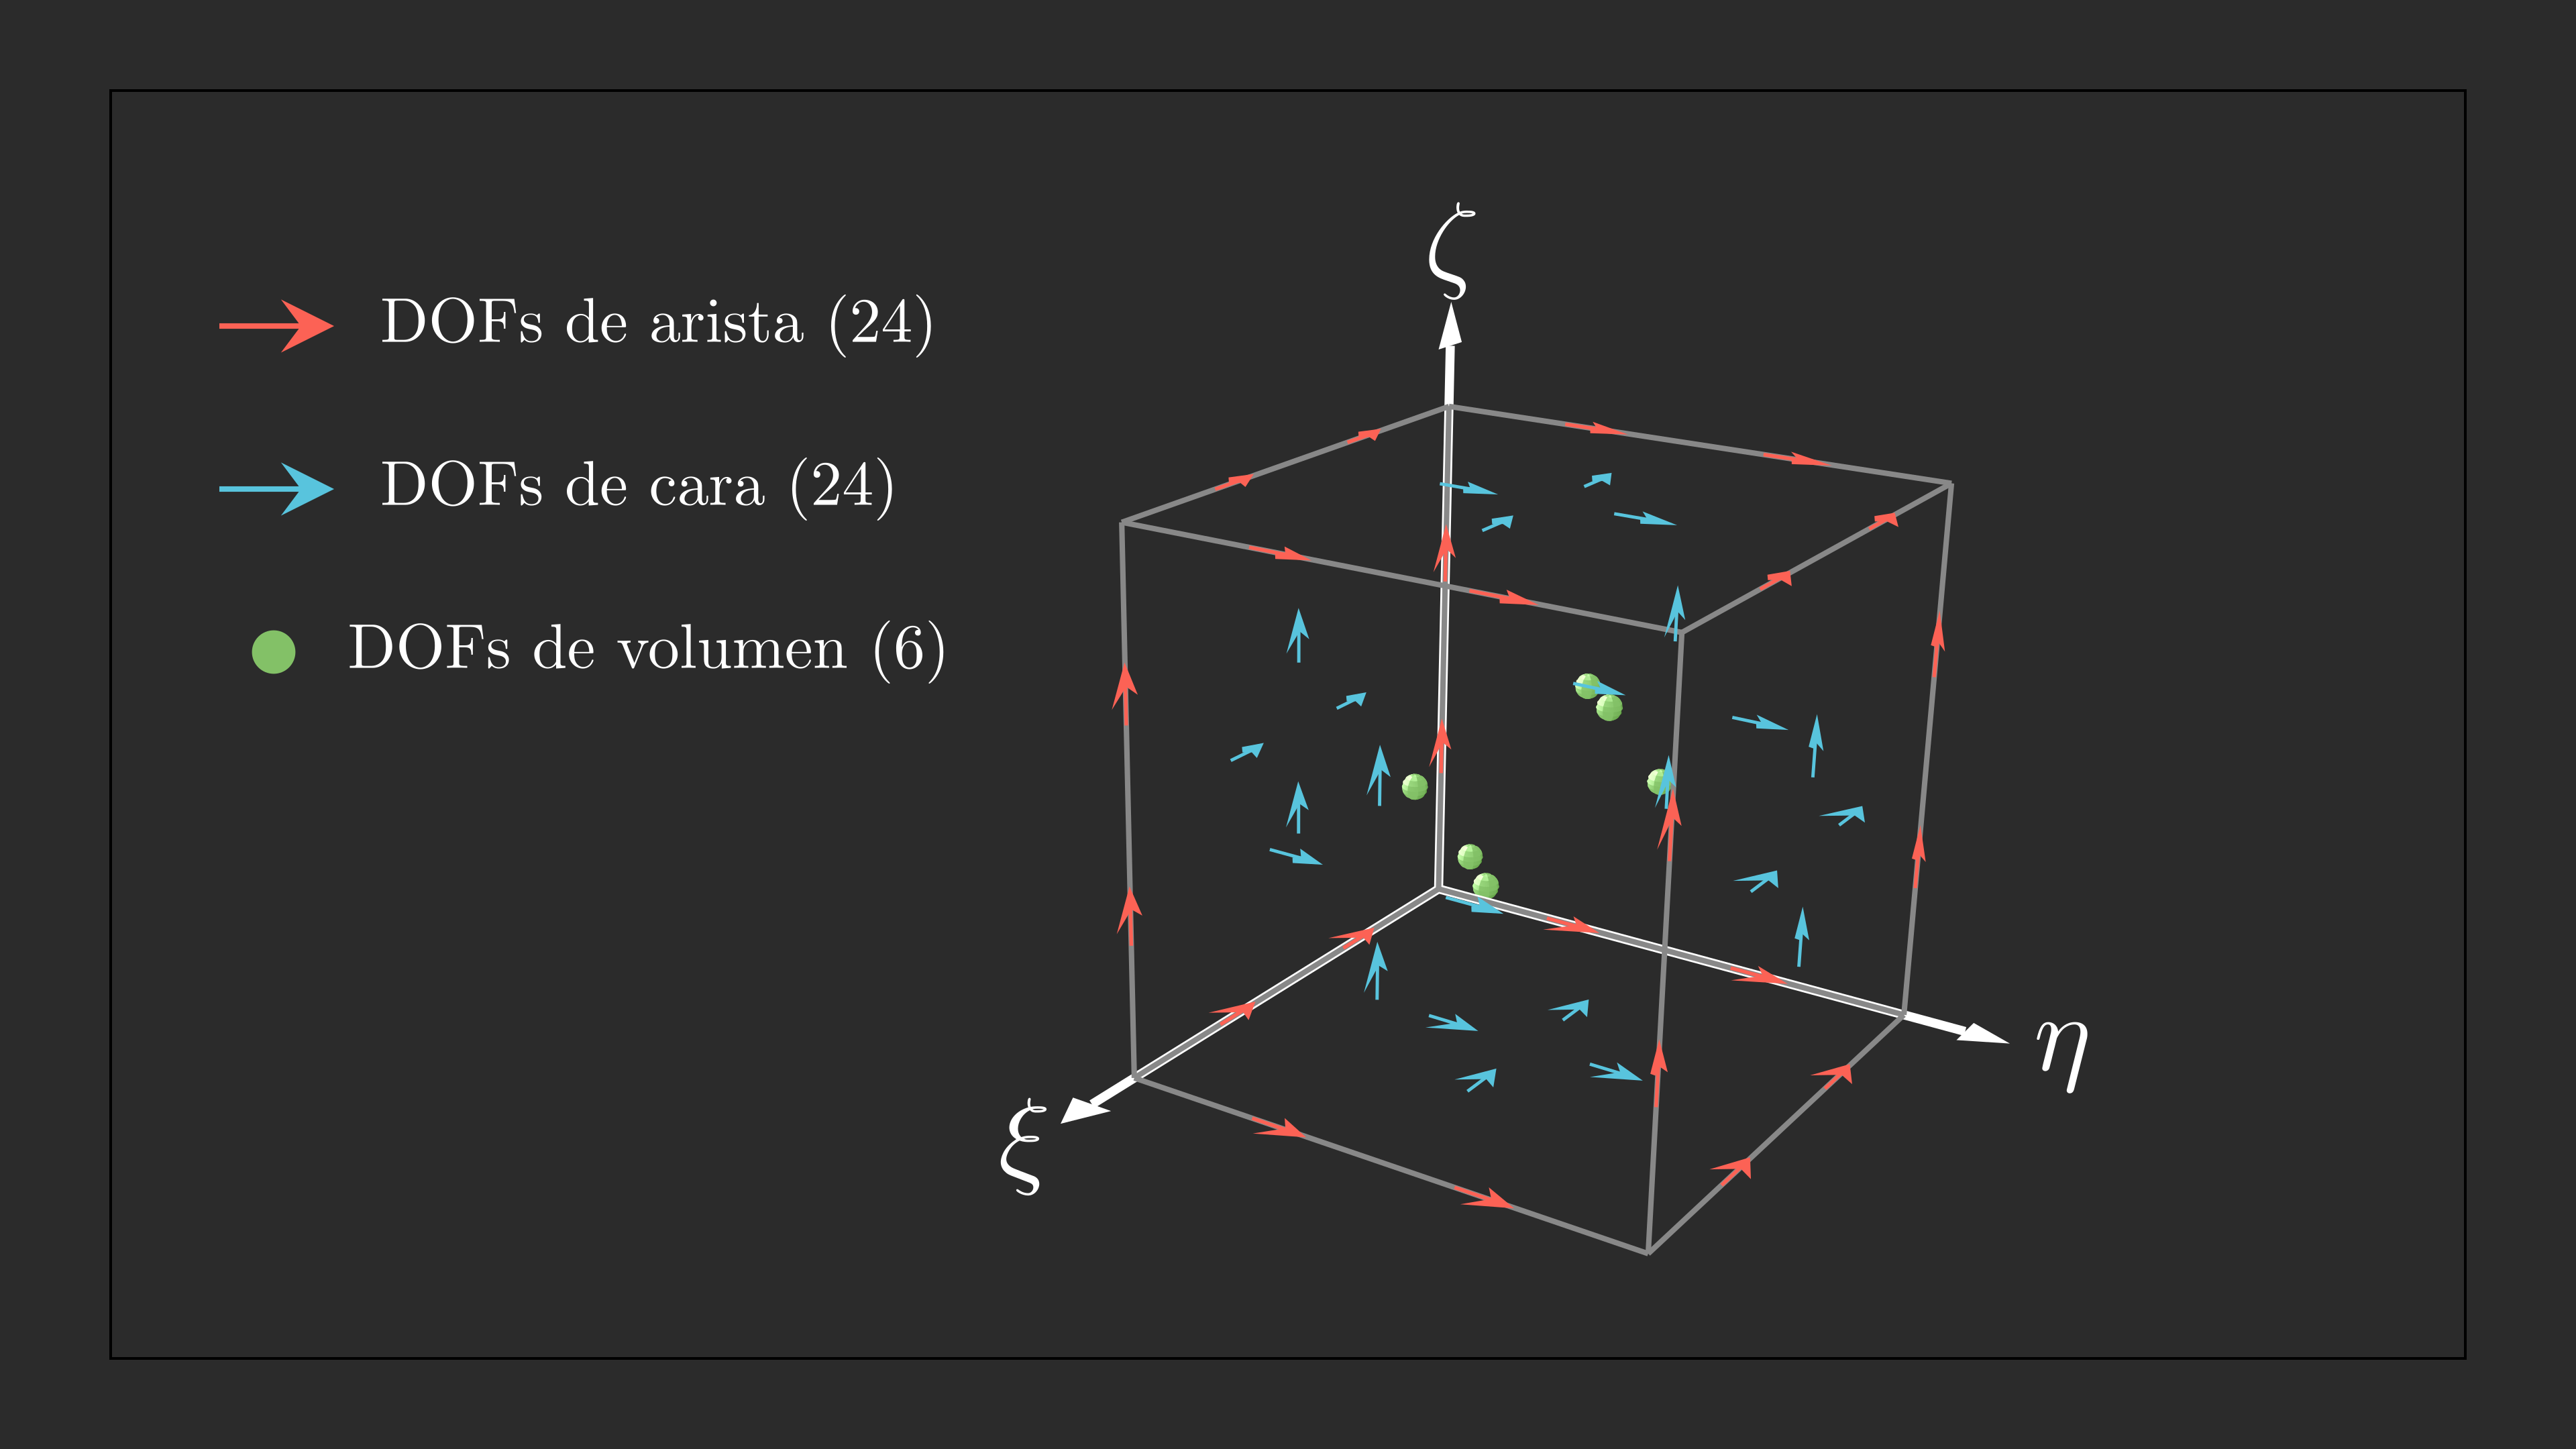
\includegraphics[width=0.9\linewidth]{hexaedro_referencia.png}
\end{figure}

\section{El espacio $\mathcal{H}_2$ y los monomios}\label{sec:h2}

Como se explicó en \autoref{sec:nedelec}, se ha de utilizar elementos de Nédélec de orden mixto. Para describirlo se usará la notaci\'on $Q_{p_1,p_2,p_3}$, para describir polinomios de hasta grado $p_1, p_2 $ y $p_3$ en $\xi$, $\eta$ y $\zeta$, respectivamente, mientras que para el caso unidimensional de grado $p$ se usará $P_p$.

Para obtener el espacio de orden $k$ en el hexaedro de referencia $H=[0,1]^3$ se hace el producto tensorial de polinomios escalares definidos a lo largo de los ejes $I_\xi$, $I_\eta$ y $I_\zeta$, de manera que la componente en la que apunta el eje sea un grado inferior:
\begin{equation}\label{eq:hk}
	\begin{aligned}
		\mathcal{H}_k =
		&\{P_{k-1}(I_\xi)\otimes P_k(I_\eta)\otimes P_k(I_\zeta)\}\\
		\times{}&\{P_k(I_\xi)\otimes P_{k-1}(I_\eta)\otimes P_k(I_\zeta)\}\\
		\times{}&\{P_k(I_\xi)\otimes P_k(I_\eta)\otimes P_{k-1}(I_\zeta)\},
	\end{aligned}
\end{equation}

Como se justific\'o en \autoref{sec:nedelec}, el orden mixto garantiza la inclusi\'on $\nabla V_h^{\text{nodal}}\subset V_h$ (\autoref{eq:gradiente-incluido}), de modo que el n\'ucleo discreto de $\mathbf{K}$ se reproduce de forma exacta y los modos espurios quedan concentrados en $k_0^2\approx 0$, bien separados del espectro f\'isico y f\'aciles de filtrar.

Para orden $2$, que es el que vamos a usar si $q\in Q_{2,2,2}$, entonces:

$\partial_\xi q\in Q_{1,2,2}$, $\partial_\eta q\in Q_{2,1,2}$ y $\partial_\zeta q\in Q_{2,2,1}$, que son los tres bloques de $\mathcal{H}_2$:
\begin{equation}\label{eq:h2}
	\mathcal{H}_2 = Q_{1,2,2} \times Q_{2,1,2} \times Q_{2,2,1},
	\qquad \dim \mathcal{H}_2 = 3 \cdot (2\cdot3\cdot3) = 54 .
\end{equation}
Por lo tanto $\nabla q\in\mathcal{H}_2$.

\begin{lstlisting}[language=Julia, caption={Construcci\'on de los 54 monomios de $\mathcal{H}_2$.}, label=cod:h2-monomios]
	
# Los 54 monomios de H₂ = Q₁,₂,₂ × Q₂,₁,₂ × Q₂,₂,₁
function build_h2_monomials()
    m = Vector{Function}()

        let kξ=kξ, kη=kη, kζ=kζ
            push!(m, (ξ, η, ζ) -> [ξ^kξ * η^kη * ζ^kζ, 0.0, 0.0])
        end
    end

    for kζ in 0:2, kη in 0:1, kξ in 0:2
        let kξ=kξ, kη=kη, kζ=kζ
            push!(m, (ξ, η, ζ) -> [0.0, ξ^kξ * η^kη * ζ^kζ, 0.0])
        end
    end

    for kζ in 0:1, kη in 0:2, kξ in 0:2
        let kξ=kξ, kη=kη, kζ=kζ
            push!(m, (ξ, η, ζ) -> [0.0, 0.0, ξ^kξ * η^kη * ζ^kζ])
        end
    end

    return m
end
\end{lstlisting}

Los 54 monomios de $\mathcal{H}_2$  quedarían como:

\begin{equation}\label{eq:h2-monomios}
	\mathcal{H}_2 =
	\begin{pmatrix}
		a_1 + a_2 \xi + a_3 \eta + a_4 \xi\eta + a_5 \eta^2 + \cdots + a_{14} \xi\zeta^2 + a_{15} \eta\zeta^2 + a_{16} \xi\eta\zeta^2 + a_{17} \eta^2\zeta^2 + a_{18} \xi\eta^2\zeta^2\\
		b_1 + b_2 \xi + b_3 \xi^2 + b_4 \eta + b_5 \xi\eta + \cdots + b_{14} \xi\zeta^2 + b_{15} \xi^2\zeta^2 + b_{16} \eta\zeta^2 + b_{17} \xi\eta\zeta^2 + b_{18} \xi^2\eta\zeta^2\\
		c_1 + c_2 \xi + c_3 \xi^2 + c_4 \eta + c_5 \xi\eta + \cdots + c_{14} \xi\eta\zeta + c_{15} \xi^2\eta\zeta + c_{16} \eta^2\zeta + c_{17} \xi\eta^2\zeta + c_{18} \xi^2\eta^2\zeta
	\end{pmatrix},
\end{equation}

\section{Grados de libertad de arista, cara y volumen}\label{sec:dofs}
Utilizamos la definición de grado de libertad que se utiliza en \cite{nedelec1980, ciarlet2002, amor2023hexahedral}. Los DOF son funcionales lineales, aplicaciones lineales que llevan un espacio de funciones en nuestro caso $\mathcal{H}_2$ a los números reales, $f:\mathcal{H}_2\longrightarrow\mathbb{R}$. Un ejemplo típico son integrales o proyecciones.

Los DOF son 54 funcionales que miden el campo eléctrico sobre las diferentes geometrías del hexaedro de referencia. Como el campo eléctrico pertenece a $H(\mathrm{curl})$, en las geometrías compartidas con otros elementos se impone la continuidad de la componente tangencial. Para el hexaedro de referencia se definen tres tipos de funcionales en función de la geometría sobre la que actúan:

\subsection{DOF de arista}\label{subsec:dof-arista}
La componente tangencial del campo a lo largo de la arista $e$ se obtiene proyectando $\mathbf{u}$ (el campo $\mathbf{E}$ en la arista) sobre $\hat{\boldsymbol{\tau}}$, el vector unitario tangente a la arista:
\begin{equation}\label{eq:proyeccion}
 \operatorname{proy}_{\hat{\boldsymbol{\tau}}}(\mathbf{u}) = (\mathbf{u}\cdot\hat{\boldsymbol{\tau}})\,\hat{\boldsymbol{\tau}},
\end{equation}
El funcional de arista es la integral de la componente escalar de esa proyecci\'on y ponderada por un polinomio $q$:
\begin{equation}\label{eq:dof-arista}
 g_i^{\text{arista}}(\mathbf{u}) = \int_{e} (\mathbf{u}\cdot\hat{\boldsymbol{\tau}})\, q \; dl,
 \qquad q\in P_1(e).
\end{equation}
Los polinomios $q$ son los dos polinomios de Lagrange de grado uno sobre la arista
\begin{equation*}
	q\in\{1-t,\; t\}.
\end{equation*}
Con 12 aristas y 2 polinomios $q$ por arista aportan $24$ DOF.

\subsection{DOF de cara}\label{subsec:dof-cara}
En el caso de la cara $f$  la componente tangencial es un vector en el plano de la cara dado por $\hat{\mathbf{n}}\times\mathbf{u}$, donde $\hat{\mathbf{n}}$ es la normal unitaria apuntando hacia fuera.
Como hemos mencionado antes el funcional es una aplicación lineal que devuelve un número real, como ahora la componente tangencial es un vector, se hace el producto escalar con $\mathbf{q}$, que ahora es también otro vector que pertenece a $\{Q_{0,1}\times Q_{1,0}\}$.
\begin{equation}\label{eq:dof-cara}
	g_i^{\text{cara}}(\mathbf{u}) = \int_{f} (\hat{\mathbf{n}}\times\mathbf{u})\cdot \mathbf{q} \; ds,
	\qquad \mathbf{q}\in\{Q_{0,1}\times Q_{1,0}\}.
\end{equation}
$\{Q_{0,1}\times Q_{1,0}\}$ garantiza el orden mixto necesario. La primera componente de $\mathbf{q}$ est\'a en $Q_{0,1}$, es decir, tiene grado $0$ en la primera coordenada y grado $1$ en la segunda mientras que la segunda componente de $\mathbf{q}$ al revés. Un ejemplo de los vectores de prueba de una cara es el siguiente:
\begin{equation*}
	\mathbf{q}\in\left\{
	\begin{pmatrix} 1 \\ 0 \end{pmatrix},\;
	\begin{pmatrix} \eta \\ 0 \end{pmatrix},\;
	\begin{pmatrix} 0 \\ 1 \end{pmatrix},\;
	\begin{pmatrix} 0 \\ \xi \end{pmatrix}
	\right\}.
\end{equation*}
Con 6 caras y 4 vectores $\mathbf{q}$ por cara aportan 24 DOF.

\subsection{DOF de volumen}\label{subsec:dof-volumen}
En el interior ya se garantiza la continuidad de la componente tangencial por lo que el  funcional mide directamente el campo multiplicado ponderado por un vector de prueba $\mathbf{q}$:
\begin{equation}\label{eq:dof-volumen}
	g_i^{\text{volumen}}(\mathbf{u}) = \int_{H} \mathbf{u}\cdot \mathbf{q} \; dV,
	\qquad \mathbf{q}\in\{Q_{1,0,0}\times Q_{0,1,0}\times Q_{0,0,1}\}.
\end{equation}
El espacio $\{Q_{1,0,0}\times Q_{0,1,0}\times Q_{0,0,1}\}$ aporta dos polinomios por componente por lo que hay 6 DOF de volumen. Los vectores de prueba son:
\begin{equation*}
	\mathbf{q}\in\left\{
	\begin{pmatrix} 1-\xi \\ 0 \\ 0 \end{pmatrix},\;
	\begin{pmatrix} \xi \\ 0 \\ 0 \end{pmatrix},\;
	\begin{pmatrix} 0 \\ 1-\eta \\ 0 \end{pmatrix},\;
	\begin{pmatrix} 0 \\ \eta \\ 0 \end{pmatrix},\;
	\begin{pmatrix} 0 \\ 0 \\ 1-\zeta \end{pmatrix},\;
	\begin{pmatrix} 0 \\ 0 \\ \zeta \end{pmatrix}
	\right\}.
\end{equation*}
En total hay $24+24+6=54$ DOF que coincide con  la $\dim\mathcal{H}_2$ de \eqref{eq:h2}. Esto permite construir la base dual $\mathbf{G}\mathbf{W}=\mathbf{I}$ de la \autoref{sec:coeficientes} y garantiza la unisolvencia de las soluciones \cite{nedelec1980, amor2023hexahedral, monk2003}.

\section{Generación de coeficientes: $\mathbf{GW}=\mathbf{I}$}\label{sec:coeficientes}
\subsection{Base dual}\label{subsec:base-dual}
Dado un espacio vectorial $V$ con dimensiones finitas se denomina espacio dual $V^*$ al  conjunto de todas las aplicaciones lineales que a cada vector $V$ le asignan un valor escalar $\varphi: V \to \mathbb{K}$. Una vez definido un espacio dual, una base dual es un conjunto de vectores que forma una base para el espacio dual de un espacio vectorial. De tal forma que dado un conjunto de vectores base de $V$ $\{\mathbf{v}_1, \dots, \mathbf{v}_n\}$ , existe una base dual $\{\mathbf{v}^*_1, \dots, \mathbf{v}^*_n\}$ que cumple con la relación
\begin{equation}\label{eq:dualidad-general}
	\mathbf{v}^*_i(\mathbf{v}_j) =
	\begin{cases}
		1 & \text{si } i = j,\\
		0 & \text{si } i \neq j,
	\end{cases}
	= \delta_{ij},
\end{equation}

Donde $\delta_{ij}$ es la delta de Kronecker. De tal manera que cada funcional $\mathbf{v}^*_i$ de la base dual devuelve 1 al evaluarlo sobre su vector asociado $\mathbf{v}_i$ y cero en el resto.

Si lo aplicamos a este trabajo, volviendo a la definición de elemento finito de Ciarlet \cite{ciarlet2002}, entonces:
\begin{align}
	K \text{ (elemento geométrico)} &= \text{hexaedro de referencia } H = [0,1]^3, \\
	P \text{ (espacio de funciones)} &= \mathcal{H}_2 \text{ (los 54 monomios)}, \\
	\Sigma_k \text{ (grados de libertad)} &= \{g_i\}_{i=1}^{54} \text{ (las 54 DOFs de cada tipo)} .
\end{align}

Para que se cumpla la condición de unisolvencia, los funcionales de $\Sigma_k$ deben  identificar de manera unívoca las funciones de $\mathcal{H}_2$, lo que equivale a que $\Sigma_k$ sea una base del espacio dual de $\mathcal{H}_2$. Para $\Sigma_k$ existe una única base dual  $\{N_j\}_{j=1}^{54}$ de $\mathcal{H}_2$ que cumple la condición de base dual expuesta anteriormente:

\begin{equation}\label{eq:dual}
 g_i(N_j) = \delta_{ij}, \qquad i,j = 1,\dots,54 .
\end{equation}

Para construir  esta base dual a partir de los monomios de $\mathcal{H}_2$, se evalúan los funcionales sobre cada monomio, generando la matriz de Gram $G$ y a su inversa $W$.

\subsection{Construcción de la matriz de Gram $G$ y su inversa $W$}\label{subsec:construccion-GW}
Para construir  esta base dual a partir de los monomios de $\mathcal{H}_2$, se evalúan los funcionales sobre cada monomio, generando la matriz de Gram $G$ y a su inversa $W$.
\begin{equation}\label{eq:G}
	G_{ij} = g_i(\mathbf{u}_j), \qquad
	\mathbf{G}\,\mathbf{W} = \mathbf{I}_{54}, \qquad
\end{equation}

La definición clásica de matriz de Gram es una matriz cuadrada resultado de todos los productos escalares de un conjunto de vectores. En este caso al utilizar funcionales como son los grados de libertad, la matriz de Gram es el resultado de $G_{ij}=g_i(\mathbf{u}_j)$ y guarda la información del resultado de aplicar el DOF i al monomio j. Se le sigue llamando de la misma manera aunque no sean productos vectoriales porque sigue guardando el mismo tipo de información, la relación entre $\mathcal{H}_2$ (los monomios) y los funcionales.


El problema que se busca resolver es construir las 54 funciones de base que cumplan:

\begin{equation*}
	g_i(\mathbf{N}_j) =  \delta_{ij},
\end{equation*}

y se sabe que las funciones de base son combinaciones lineales de monomios $u_k$ ponderados por unos coeficientes $W_{kj}$

\begin{equation*}
	\mathbf{N}_j= \sum_{k=1}^{54} W_{kj}\ u_k
\end{equation*}

Donde los coeficientes $W_{kj}$ son lo que buscamos resolver. Aplicando los funcionales a ambos lados y sustituyendo $ G_{ij} = g_i(\mathbf{u}_j) $:
\begin{equation*}
	g_i(\mathbf{N}_j) = \sum_{k=1}^{54} W_{kj}\, g_i(\mathbf{u}_k) = \sum_{k=1}^{54} W_{kj}\, G_{ik} = (\mathbf{G}\mathbf{W})_{ij} = \delta_{ij},
\end{equation*}

Por lo que para calcular los coeficientes basta con aplicar las funciones de base a los monomios para calcular la matriz de Gram y luego invertirla $W = G^{-1}$.

\begin{lstlisting}[language=Julia, caption={Construcci\'on de la base dual $\mathbf{G}\mathbf{W}=\mathbf{I}$ a partir de los funcionales de la \autoref{sec:dofs}.}, label=cod:coeficientes]
	function get_coefficients()
	    monomials = build_h2_monomials()      # los 54 monomios de H2
	    N = length(monomials)
	    G = zeros(N, N)
	    for j in 1:N
	        G[:, j] = evaluate_all_dofs(monomials[j])   # g_i(u_j)
	    end
	    W = G \ I(N)                          # W = G^{-1}
	    return W, G
	end
\end{lstlisting}

\subsection{Coeficientes enteros}\label{subsec:coeficientes-enteros}
En \autoref{tab:W} se muestra el resultado del código anterior y se puede ver que todos los coeficientes de la tabla son enteros y menores en valor absoluto a 216. Este resultado indica tanto que las evaluaciones de los monomios que se calculan mediante coma flotante son correctas como que la matriz está bien construida. Además, al ser enteros, los coeficientes se representan de forma exacta en coma flotante, lo que evita errores de redondeo al almacenarlos.

\clearpage
\begin{center}
	\scriptsize
	\renewcommand{\arraystretch}{0.75}
	\setlength{\tabcolsep}{2.5pt}

	\begin{tabular}{||>{\centering\arraybackslash}p{0.55cm}|>{\centering\arraybackslash}p{0.55cm}|>{\centering\arraybackslash}p{0.55cm}|>{\centering\arraybackslash}p{0.55cm}|>{\centering\arraybackslash}p{0.55cm}|>{\centering\arraybackslash}p{0.55cm}|>{\centering\arraybackslash}p{0.55cm}|>{\centering\arraybackslash}p{0.55cm}|>{\centering\arraybackslash}p{0.55cm}|>{\centering\arraybackslash}p{0.55cm}|>{\centering\arraybackslash}p{0.55cm}|>{\centering\arraybackslash}p{0.55cm}|>{\centering\arraybackslash}p{0.55cm}|>{\centering\arraybackslash}p{0.55cm}|>{\centering\arraybackslash}p{0.55cm}|>{\centering\arraybackslash}p{0.55cm}|>{\centering\arraybackslash}p{0.55cm}|>{\centering\arraybackslash}p{0.55cm}||}
	\hline\hline
$N_{1}$ & $N_{2}$ & $N_{3}$ & $N_{4}$ & $N_{5}$ & $N_{6}$ & $N_{7}$ & $N_{8}$ & $N_{9}$ & $N_{10}$ & $N_{11}$ & $N_{12}$ & $N_{13}$ & $N_{14}$ & $N_{15}$ & $N_{16}$ & $N_{17}$ & $N_{18}$ \\
\hline\hline
$\xi$ & $\xi$ & $\eta$ & $\eta$ & $\eta$ & $\eta$ & $\eta$ & $\eta$ & $\xi$ & $\xi$ & $\eta$ & $\eta$ & $\xi$ & $\xi$ & $\eta$ & $\eta$ & $\zeta$ & $\zeta$ \\
\hline\hline
4 & -2 & 0 & 0 & 0 & 0 & 4 & -2 & 0 & 0 & 0 & 0 & 0 & 0 & 0 & 0 & 4 & -2 \\
-6 & 6 & -8 & 4 & 0 & 0 & -16 & 8 & 0 & 0 & 0 & 0 & 0 & 0 & 0 & 0 & -16 & 8 \\
-16 & 8 & 12 & -6 & -8 & 4 & 12 & -6 & 0 & 0 & 0 & 0 & 0 & 0 & 0 & 0 & 12 & -6 \\
24 & -24 & 0 & 0 & 12 & -12 & -6 & 6 & 0 & 0 & 0 & 0 & 0 & 0 & 0 & 0 & -16 & 8 \\
12 & -6 & 12 & -12 & 12 & -6 & 24 & -24 & 0 & 0 & 0 & 0 & 0 & 0 & 0 & 0 & 64 & -32 \\
-18 & 18 & -18 & 18 & -18 & 18 & -18 & 18 & 0 & 0 & 0 & 0 & 0 & 0 & 0 & 0 & -48 & 24 \\
-16 & 8 & 0 & 0 & 0 & 0 & -16 & 8 & -8 & 4 & 0 & 0 & 0 & 0 & -8 & 4 & 12 & -6 \\
24 & -24 & 32 & -16 & 0 & 0 & 64 & -32 & 12 & -12 & 16 & -8 & 0 & 0 & 32 & -16 & -48 & 24 \\
64 & -32 & -48 & 24 & 32 & -16 & -48 & 24 & 32 & -16 & -24 & 12 & 16 & -8 & -24 & 12 & 36 & -18 \\
-96 & 96 & 0 & 0 & -48 & 48 & 24 & -24 & -48 & 48 & 0 & 0 & -24 & 24 & 12 & -12 & -6 & 6 \\
-48 & 24 & -48 & 48 & -48 & 24 & -96 & 96 & -24 & 12 & -24 & 24 & -24 & 12 & -48 & 48 & 24 & -24 \\
72 & -72 & 72 & -72 & 72 & -72 & 72 & -72 & 36 & -36 & 36 & -36 & 36 & -36 & 36 & -36 & -18 & 18 \\
12 & -6 & 0 & 0 & 0 & 0 & 12 & -6 & 12 & -6 & 0 & 0 & 0 & 0 & 12 & -6 & 24 & -24 \\
-18 & 18 & -24 & 12 & 0 & 0 & -48 & 24 & -18 & 18 & -24 & 12 & 0 & 0 & -48 & 24 & -96 & 96 \\
-48 & 24 & 36 & -18 & -24 & 12 & 36 & -18 & -48 & 24 & 36 & -18 & -24 & 12 & 36 & -18 & 72 & -72 \\
72 & -72 & 0 & 0 & 36 & -36 & -18 & 18 & 72 & -72 & 0 & 0 & 36 & -36 & -18 & 18 & -18 & 18 \\
36 & -18 & 36 & -36 & 36 & -18 & 72 & -72 & 36 & -18 & 36 & -36 & 36 & -18 & 72 & -72 & 72 & -72 \\
-54 & 54 & -54 & 54 & -54 & 54 & -54 & 54 & -54 & 54 & -54 & 54 & -54 & 54 & -54 & 54 & -54 & 54 \\
\hline
	\end{tabular}
	\vspace{0.15cm}

	\begin{tabular}{||>{\centering\arraybackslash}p{0.55cm}|>{\centering\arraybackslash}p{0.55cm}|>{\centering\arraybackslash}p{0.55cm}|>{\centering\arraybackslash}p{0.55cm}|>{\centering\arraybackslash}p{0.55cm}|>{\centering\arraybackslash}p{0.55cm}|>{\centering\arraybackslash}p{0.55cm}|>{\centering\arraybackslash}p{0.55cm}|>{\centering\arraybackslash}p{0.55cm}|>{\centering\arraybackslash}p{0.55cm}|>{\centering\arraybackslash}p{0.55cm}|>{\centering\arraybackslash}p{0.55cm}|>{\centering\arraybackslash}p{0.55cm}|>{\centering\arraybackslash}p{0.55cm}|>{\centering\arraybackslash}p{0.55cm}|>{\centering\arraybackslash}p{0.55cm}|>{\centering\arraybackslash}p{0.55cm}|>{\centering\arraybackslash}p{0.55cm}||}
	\hline\hline
$N_{19}$ & $N_{20}$ & $N_{21}$ & $N_{22}$ & $N_{23}$ & $N_{24}$ & $N_{25}$ & $N_{26}$ & $N_{27}$ & $N_{28}$ & $N_{29}$ & $N_{30}$ & $N_{31}$ & $N_{32}$ & $N_{33}$ & $N_{34}$ & $N_{35}$ & $N_{36}$ \\
\hline\hline
$\zeta$ & $\zeta$ & $\zeta$ & $\zeta$ & $\zeta$ & $\zeta$ & $\xi$ & $\xi$ & $\eta$ & $\eta$ & $\xi$ & $\xi$ & $\eta$ & $\eta$ & $\xi$ & $\xi$ & $\zeta$ & $\zeta$ \\
\hline\hline
0 & 0 & 0 & 0 & 0 & 0 & 0 & 0 & 0 & 0 & 0 & 0 & 0 & 0 & 0 & 0 & 0 & 0 \\
-8 & 4 & 0 & 0 & 0 & 0 & 0 & 0 & 24 & -12 & 0 & 0 & 0 & 0 & 0 & 0 & 24 & -12 \\
12 & -6 & 0 & 0 & 0 & 0 & 24 & -12 & -24 & 12 & 0 & 0 & 0 & 0 & 0 & 0 & -24 & 12 \\
0 & 0 & 0 & 0 & -8 & 4 & -36 & 36 & 0 & 0 & 0 & 0 & 0 & 0 & 0 & 0 & 0 & 0 \\
32 & -16 & 16 & -8 & 32 & -16 & -24 & 12 & -36 & 36 & 0 & 0 & 0 & 0 & 0 & 0 & -96 & 48 \\
-48 & 24 & -24 & 12 & -24 & 12 & 36 & -36 & 36 & -36 & 0 & 0 & 0 & 0 & 0 & 0 & 96 & -48 \\
0 & 0 & 0 & 0 & 12 & -6 & 0 & 0 & 0 & 0 & 0 & 0 & 0 & 0 & 24 & -12 & 0 & 0 \\
-24 & 12 & -24 & 12 & -48 & 24 & 0 & 0 & -96 & 48 & 0 & 0 & -48 & 24 & -36 & 36 & 72 & -36 \\
36 & -18 & 36 & -18 & 36 & -18 & -96 & 48 & 96 & -48 & -48 & 24 & 48 & -24 & -96 & 48 & -72 & 36 \\
0 & 0 & 0 & 0 & 0 & 0 & 144 & -144 & 0 & 0 & 72 & -72 & 0 & 0 & 144 & -144 & 0 & 0 \\
12 & -12 & 0 & 0 & 0 & 0 & 96 & -48 & 144 & -144 & 48 & -24 & 72 & -72 & 72 & -36 & -36 & 36 \\
-18 & 18 & 0 & 0 & 0 & 0 & -144 & 144 & -144 & 144 & -72 & 72 & -72 & 72 & -108 & 108 & 36 & -36 \\
0 & 0 & 0 & 0 & 12 & -12 & 0 & 0 & 0 & 0 & 0 & 0 & 0 & 0 & -24 & 12 & 0 & 0 \\
-48 & 48 & -24 & 24 & -48 & 48 & 0 & 0 & 72 & -36 & 0 & 0 & 72 & -36 & 36 & -36 & 144 & -144 \\
72 & -72 & 36 & -36 & 36 & -36 & 72 & -36 & -72 & 36 & 72 & -36 & -72 & 36 & 96 & -48 & -144 & 144 \\
0 & 0 & 0 & 0 & -18 & 18 & -108 & 108 & 0 & 0 & -108 & 108 & 0 & 0 & -144 & 144 & 0 & 0 \\
36 & -36 & 36 & -36 & 72 & -72 & -72 & 36 & -108 & 108 & -72 & 36 & -108 & 108 & -72 & 36 & -108 & 108 \\
-54 & 54 & -54 & 54 & -54 & 54 & 108 & -108 & 108 & -108 & 108 & -108 & 108 & -108 & 108 & -108 & 108 & -108 \\
\hline
	\end{tabular}
	\vspace{0.15cm}

	\begin{tabular}{||>{\centering\arraybackslash}p{0.55cm}|>{\centering\arraybackslash}p{0.55cm}|>{\centering\arraybackslash}p{0.55cm}|>{\centering\arraybackslash}p{0.55cm}|>{\centering\arraybackslash}p{0.55cm}|>{\centering\arraybackslash}p{0.55cm}|>{\centering\arraybackslash}p{0.55cm}|>{\centering\arraybackslash}p{0.55cm}|>{\centering\arraybackslash}p{0.55cm}|>{\centering\arraybackslash}p{0.55cm}|>{\centering\arraybackslash}p{0.55cm}|>{\centering\arraybackslash}p{0.55cm}|>{\centering\arraybackslash}p{0.55cm}|>{\centering\arraybackslash}p{0.55cm}|>{\centering\arraybackslash}p{0.55cm}|>{\centering\arraybackslash}p{0.55cm}|>{\centering\arraybackslash}p{0.55cm}|>{\centering\arraybackslash}p{0.55cm}||}
	\hline\hline
$N_{37}$ & $N_{38}$ & $N_{39}$ & $N_{40}$ & $N_{41}$ & $N_{42}$ & $N_{43}$ & $N_{44}$ & $N_{45}$ & $N_{46}$ & $N_{47}$ & $N_{48}$ & $N_{49}$ & $N_{50}$ & $N_{51}$ & $N_{52}$ & $N_{53}$ & $N_{54}$ \\
\hline\hline
$\eta$ & $\eta$ & $\zeta$ & $\zeta$ & $\xi$ & $\xi$ & $\zeta$ & $\zeta$ & $\eta$ & $\eta$ & $\zeta$ & $\zeta$ & $\xi$ & $\xi$ & $\eta$ & $\eta$ & $\zeta$ & $\zeta$ \\
\hline\hline
0 & 0 & 0 & 0 & 0 & 0 & 0 & 0 & 0 & 0 & 0 & 0 & 0 & 0 & 0 & 0 & 0 & 0 \\
0 & 0 & 0 & 0 & 0 & 0 & 0 & 0 & 0 & 0 & 0 & 0 & 0 & 0 & 0 & 0 & 0 & 0 \\
0 & 0 & 0 & 0 & 0 & 0 & 0 & 0 & 0 & 0 & 0 & 0 & 0 & 0 & 0 & 0 & 0 & 0 \\
0 & 0 & 0 & 0 & 0 & 0 & 0 & 0 & 0 & 0 & 24 & -12 & 0 & 0 & 0 & 0 & 0 & 0 \\
0 & 0 & -48 & 24 & 0 & 0 & -48 & 24 & 0 & 0 & -96 & 48 & 0 & 0 & 0 & 0 & 144 & -72 \\
0 & 0 & 72 & -36 & 0 & 0 & 48 & -24 & 0 & 0 & 72 & -36 & 0 & 0 & 0 & 0 & -144 & 72 \\
0 & 0 & 0 & 0 & 0 & 0 & 0 & 0 & 24 & -12 & -24 & 12 & 0 & 0 & 0 & 0 & 0 & 0 \\
-48 & 24 & 48 & -24 & 0 & 0 & 72 & -36 & -96 & 48 & 96 & -48 & 0 & 0 & 144 & -72 & -144 & 72 \\
72 & -36 & -72 & 36 & -48 & 24 & -72 & 36 & 72 & -36 & -72 & 36 & 144 & -72 & -144 & 72 & 144 & -72 \\
0 & 0 & 0 & 0 & 72 & -72 & 0 & 0 & -36 & 36 & 0 & 0 & -216 & 216 & 0 & 0 & 0 & 0 \\
72 & -72 & 0 & 0 & 72 & -36 & 0 & 0 & 144 & -144 & 0 & 0 & -144 & 72 & -216 & 216 & 0 & 0 \\
-108 & 108 & 0 & 0 & -108 & 108 & 0 & 0 & -108 & 108 & 0 & 0 & 216 & -216 & 216 & -216 & 0 & 0 \\
0 & 0 & 0 & 0 & 0 & 0 & 0 & 0 & -24 & 12 & -36 & 36 & 0 & 0 & 0 & 0 & 0 & 0 \\
48 & -24 & 72 & -72 & 0 & 0 & 72 & -72 & 96 & -48 & 144 & -144 & 0 & 0 & -144 & 72 & -216 & 216 \\
-72 & 36 & -108 & 108 & 48 & -24 & -72 & 72 & -72 & 36 & -108 & 108 & -144 & 72 & 144 & -72 & 216 & -216 \\
0 & 0 & 0 & 0 & -72 & 72 & 0 & 0 & 36 & -36 & 36 & -36 & 216 & -216 & 0 & 0 & 0 & 0 \\
-72 & 72 & -72 & 72 & -72 & 36 & -108 & 108 & -144 & 144 & -144 & 144 & 144 & -72 & 216 & -216 & 216 & -216 \\
108 & -108 & 108 & -108 & 108 & -108 & 108 & -108 & 108 & -108 & 108 & -108 & -216 & 216 & -216 & 216 & -216 & 216 \\
\hline
	\end{tabular}

	\captionof{table}{Coeficientes de la matriz $W$ para los 54 grados de libertad del elemento de referencia (arista, cara y volumen), correspondientes a las funciones de base de $\mathcal{H}_2$ (Tabla II del articulo de referencia).}
	\label{tab:W}
\end{center}


\section{Evaluación en el elemento real}\label{sec:evaluacion}
Se pueden aplicar estos resultados a cualquier hexaedro, sin embargo es más eficiente primero aplicarlo a un elemento de referencia y posteriormente pasarlo al elemento real mediante la matriz jacobiana y las transformaciones de Piola.

\subsection{Mapeo isoparamétrico y matriz jacobiana}\label{sec:jacobiano}

Para pasar a los hexaedros reales de la malla es necesario conocer la relación geométrica entre el elemento de referencia y el real. Esta relación se define mediante el llamado mapeo isoparamétrico \cite{jin2015}:

\begin{align}
 x &= \sum_{i=1}^{n_e} N_i^e(\xi,\eta,\zeta)\, x_i, \label{eq:mapa-x}\\
 y &= \sum_{i=1}^{n_e} N_i^e(\xi,\eta,\zeta)\, y_i, \label{eq:mapa-y}\\
 z &= \sum_{i=1}^{n_e} N_i^e(\xi,\eta,\zeta)\, z_i, \label{eq:mapa-z}
\end{align}
donde $(x,y,z)$ son las coordenadas del elemento real, $(\xi,\eta,\zeta)$ las del elemento de referencia, $n_e$ es el número de nodos del elemento, $N_i^e$ son las funciones de forma del hexaedro y $(x_i,y_i,z_i)$ las coordenadas nodales.

\begin{figure}[H]
	\centering
	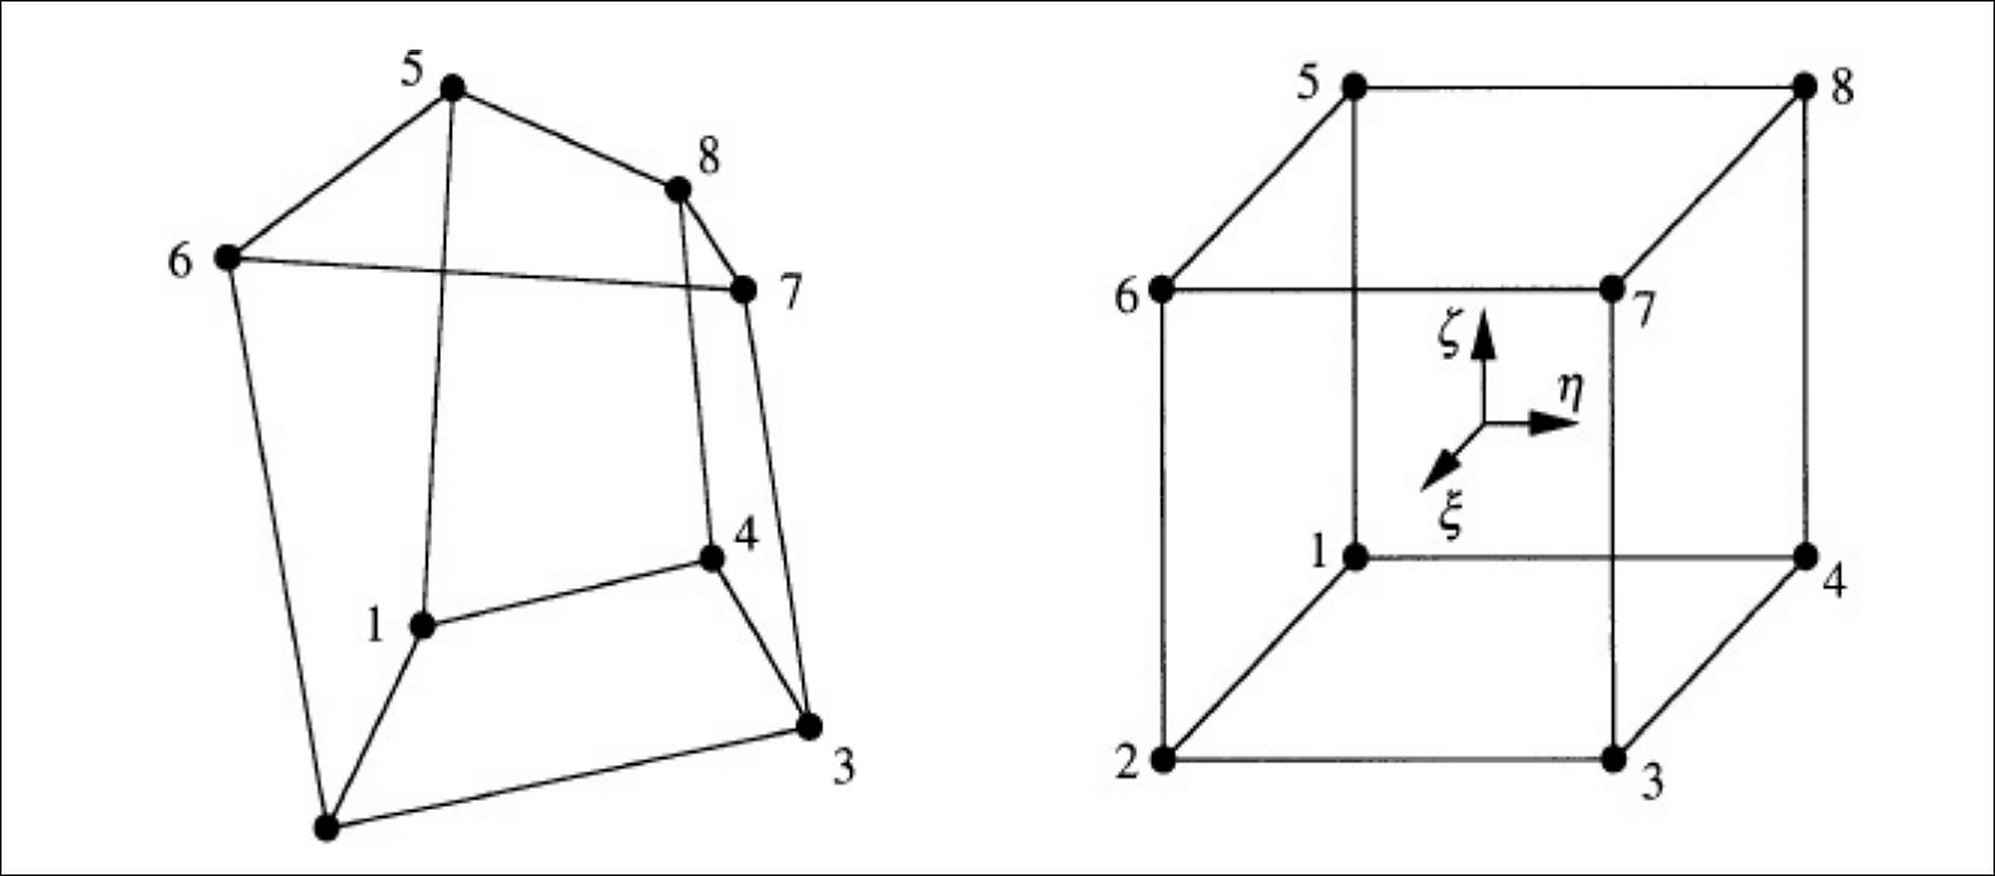
\includegraphics[width=0.85\linewidth]{imagenes/jianming_jin_upscaled.png}
	\caption[Elemento de referencia y elemento real]{Elemento de referencia en coordenadas $\xi\eta\zeta$ y elemento real en coordenadas $xyz$. Imagen sacada de la Fig.~5.6 de \cite{jin2015}, Sección~5.5.}
	\label{fig:hexaedros-transformacion}
\end{figure}

Cabe recalcar que las integrales que se resuelven en FEM (como la matriz de rigidez) necesitan las derivadas de las funciones de base respecto de las coordenadas reales $(x,y,z)$. Por lo tanto es necesario relacionar las derivadas respecto de las coordenadas reales con las derivadas respecto de las coordenadas de referencia $(\xi,\eta,\zeta)$. Esta relación viene dada por la matriz jacobiana, cuyas columnas son las derivadas del mapeo isoparamétrico:
\begin{equation}\label{eq:jacobiana}
 [J] = \begin{bmatrix}
 	\frac{\partial x}{\partial \xi} & \frac{\partial y}{\partial \xi} & \frac{\partial z}{\partial \xi} \\[2pt]
 	\frac{\partial x}{\partial \eta} & \frac{\partial y}{\partial \eta} & \frac{\partial z}{\partial \eta} \\[2pt]
 	\frac{\partial x}{\partial \zeta} & \frac{\partial y}{\partial \zeta} & \frac{\partial z}{\partial \zeta}
 \end{bmatrix},
\end{equation}

Por la regla de la cadena, las derivadas de una función escalar (como las
funciones de forma o de base) en coordenadas reales se relacionan
con sus derivadas en el eje de referencia mediante la inversa
de la matriz jacobiana (Ec.~5.56 de \cite{jin2015}):
\begin{equation}\label{eq:derivadas-forma}
 \begin{Bmatrix}
 	\frac{\partial N_i^e}{\partial x} \\[2pt]
 	\frac{\partial N_i^e}{\partial y} \\[2pt]
 	\frac{\partial N_i^e}{\partial z}
 \end{Bmatrix}
 = [J]^{-1}
 \begin{Bmatrix}
 	\frac{\partial N_i^e}{\partial \xi} \\[2pt]
 	\frac{\partial N_i^e}{\partial \eta} \\[2pt]
 	\frac{\partial N_i^e}{\partial \zeta}
 \end{Bmatrix}.
\end{equation}


\subsection{Transformación de Piola covariante y contravariante}\label{sec:piola}
Para las funciones de base vectoriales que deben mantener la continuidad de la componente tangencial, necesaria en $H(\mathrm{curl})$, se utiliza la transformación de Piola covariante.

\begin{equation}\label{eq:piola-cov}
	\mathbf{N} = \mathbf{J}^{-T}\, \hat{\mathbf{N}} .
\end{equation}
La transformación de Piola contravariante permite obtener el rotacional de las funciones de base $\nabla\times\mathbf{N}$ a partir del rotacional de la base
de referencia, utilizando el jacobiano calculado anteriormente y evitando así derivar numéricamente
\begin{equation}\label{eq:piola-contra}
	\nabla\times\mathbf{N} = \frac{1}{\det \mathbf{J}}\, \mathbf{J}\,
	(\hat{\nabla}\times\hat{\mathbf{N}}) .
\end{equation}
Con el mapeo isoparamétrico y las transformaciones de Piola se puede evaluar en el elemento real sin tener que calcular coeficientes para cada geometría.

\section{Mallado y etiquetado}\label{sec:mallado}

Para poder ensamblar el sistema como ya se expuso en \autoref{subsec:mef-discretizacion} el primer paso es discretizar el dominio $\Omega$ en subdominios para lo cual se han utilizado 2 métodos distintos. El primero es utilizar directamente las mallas de la implementación de MATLAB \cite{amor2022zenodo} y la otra posibilidad es generar mallas con gmsh, utilizando la estructura heredada de MATLAB que añade etiquetas a cada elemento según su condición de contorno y material.

\subsection{Generación y etiquetado de las mallas con Gmsh}\label{sec:gmsh}

la función que implementa la generación de las mallas es \texttt{box\_mesh} que genera una caja de dimensiones  $[0,L_x]\times[0,L_y]\times[0,L_z]$ que se divide en $n_x\times n_y\times n_z$ hexaedros transfinitos (con un número fijo de divisiones sobre las diferentes geometrías) que generan una malla estructurada (todas las aristas paralelas a un mismo eje
reciben el mismo número de divisiones) \cite{gmshmanual}. Las mallas tienen etiquetas de contorno (\texttt{PolyFace}) que agrupan aristas y caras que comparten una misma condición de contorno y una etiqueta de material (\texttt{Solid}) que agrupa elementos con el mismo $\varepsilon_r$ y $\mu_r$. En el ensamblaje solo se usan las etiquetas y no infiere datos según la topología.
El siguiente pseudocódigo resume los pasos de la función \texttt{box\_mesh} para generar mallas.

\begin{lstlisting}[language=Julia, captionpos=b, caption={Pseudoc\'odigo de la generaci\'on y etiquetado de una malla hexa\'edrica estructurada con \texttt{box\_mesh}.}, label=cod:generacion-malla]
# --- Generacion de la geometria y la malla ---
# 1. Caja [0,Lx]x[0,Ly]x[0,Lz]
caja = addBox(0, 0, 0, Lx, Ly, Lz)

# 2. Divisiones transfinitas por arista (malla estructurada)
for cada arista:
    setTransfiniteCurve(arista, n_dir + 1)   # n_dir = nx, ny o nz

# 3. Recombinar triangulos en cuadrilateros/hexaedros (gmsh no genera hexaedros directamente)
for cada cara:  setTransfiniteSurface(cara);  setRecombine(cara)
setTransfiniteVolume(caja)

# 4. Generar la malla y leer nodos y hexaedros
mesh.generate(3);  mesh.recombine()
nodos, hexaedros = getNodes(), getElements(hex8)

# 5. Reordenar los nodos de cada hexaedro al convenio de ReferenceHex
reordenar cada hexaedro con [3,7,8,4,2,6,5,1]

# 6. Condicion de contorno: declarar el contorno como grupo fisico de Gmsh y
#    guardar sus caras y aristas en face_polyface/edge_polyface.
#    (En este trabajo solo PEC en el exterior.)
grupo = addPhysicalGroup(superficies exteriores, nombre="contorno", tipo="PerfectE")
for cada cuadrilatero del grupo:
    face_polyface[ordenar(nodos)] = id
    edge_polyface[ordenar(arista)] = id

# 7. Material: asignar cada elemento a un Solid con tag_solids_by_plane!
#    (En este trabajo solo la cavidad semillena: dieléctrico abajo, vacío arriba.)
tag_solids_by_plane!(malla; axis=:z, cut=cut,
                     below=("dielectrico", 2.0, 1.0), above=("vacio", 1.0, 1.0))

devolver HexMesh(nodos, hexaedros, element_solid, face_polyface, edge_polyface)
\end{lstlisting}
La función devuelve una estructura \texttt{HexMesh} que contiene las coordenadas de los nodos, de los elementos y las etiquetas de material y de las condiciones de contorno de caras y aristas.



\begin{figure}[H]
	\centering
	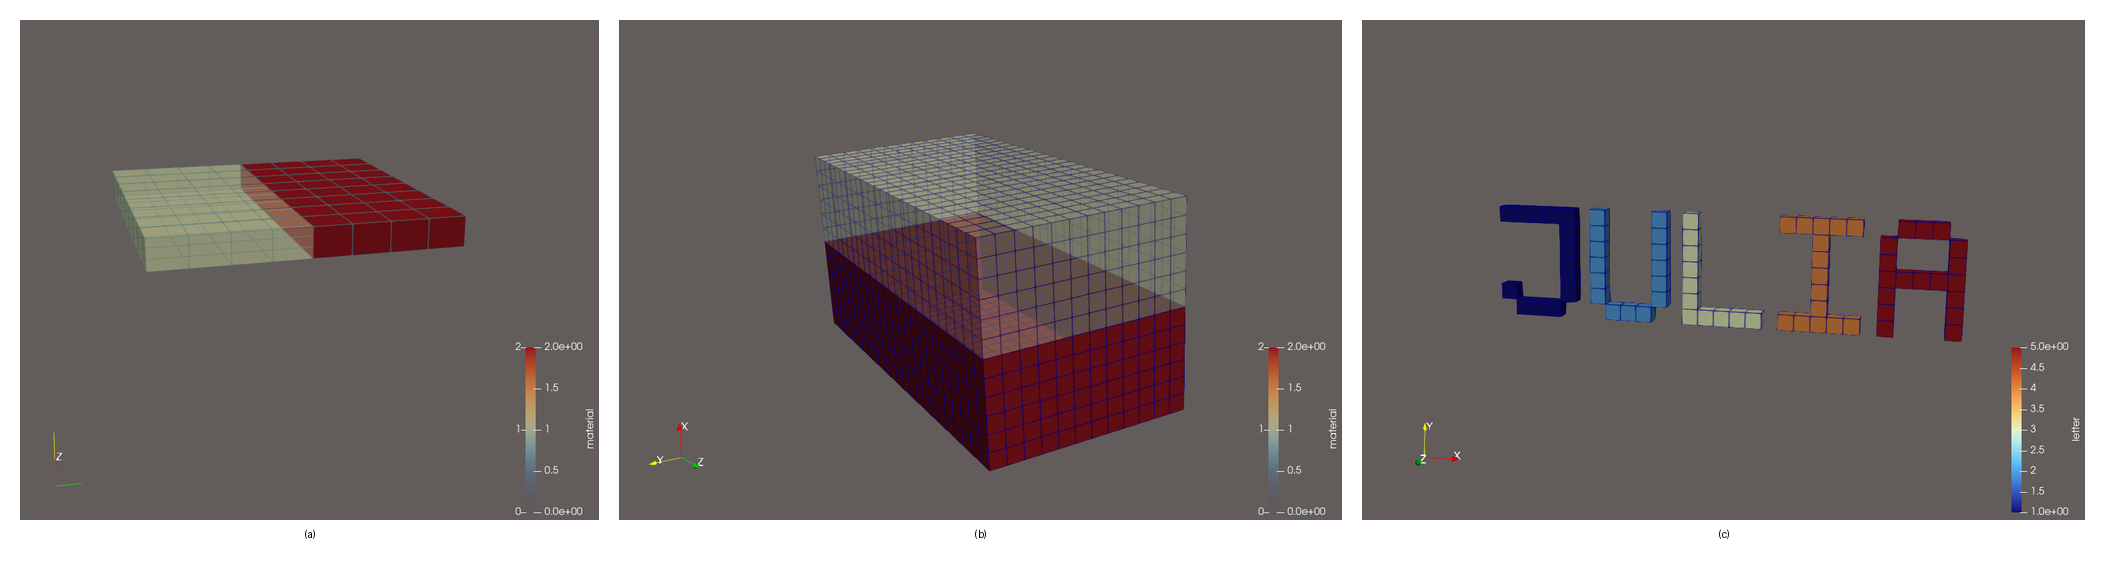
\includegraphics[width=\linewidth]{mallas_combinadas.png}
	\caption{Ejemplos de mallas hexaédricas estructuradas generadas con Gmsh:
		(a) malla exportada de MATLAB, (b) cavidad semillena rectangular generada con gmsh y
		(c) malla que forma la palabra \emph{JULIA} también generada con gmsh.}
	\label{fig:mallas}
\end{figure}

\section{Ensamblaje del sistema}\label{sec:ensamblaje}

\subsection{Numeración global de grados de libertad}\label{sec:dofs-globales}

Al generar una malla cada elemento aporta 54 DOF, sin embargo, elementos adyacentes comparten grados de libertad. Con el objetivo de ensamblar un sistema con incógnitas únicas las geometrías compartidas (aristas y caras) deben tener el mismo DOF.

El módulo encargado de la numeración global es \texttt{GlobalDOFs.jl} en concreto la función \texttt{build\_dof\_map}. Recorre la malla elemento a elemento y, para cada uno, procesa sus 54 DOFs en tres grupos: los de arista, los de cara y los de volumen. Para los de arista crea una clave única con los nodos ordenados de menor a mayor \texttt{key = minmax(gn1, gn2)} si esa clave no está añadida al diccionario se reservan 2 Dof globales y se añade al diccionario. Para las caras es lo mismo pero con los 4 nodos de la cara ordenados \texttt{key = NTuple{4,Int}(sort!(collect(gfn)))}. Por último, los de volumen siempre se añaden, ya que no se pueden compartir entre elementos.

Cuando termina de identificar los DOF globales únicos \texttt{build\_dof\_map} devuelve el número total de grados de libertad \texttt{n\_dofs} y \texttt{connectivity} que es una matriz de enteros de dimensiones \texttt{n\_elementos} x 54 que incluye los DOF globales únicos de cada elemento.

Este es de los pocos módulos sin una correspondencia directa con MATLAB porque se utiliza programación orientada a objetos. En MATLAB las aristas y caras comunes a dos elementos son el mismo objeto y se comparten por referencia, mientras que en Julia la malla es un array de conectividad y las aristas y caras se reconocen utilizando sus claves guardadas en diccionarios.

\subsection{Matrices de rigidez y masa}\label{sec:KM}
En \autoref{subsec:mef-sistema} definimos la forma débil del problema de autovalores donde se busca $\mathbf{E}$ tal que, para toda función de prueba $\mathbf{v}\in H_0(\mathrm{curl},\Omega)$,
\begin{equation}\label{eq:forma-debil-KM}
	\int_\Omega \frac{1}{\mu_r}(\nabla\times\mathbf{E})\cdot(\nabla\times\mathbf{v})\,d\Omega
	- k_0^2 \int_\Omega \varepsilon_r\,\mathbf{E}\cdot\mathbf{v}\,d\Omega = 0 .
\end{equation}

Este problema era para el dominio completo. Si ahora se quiere aplicar a los subdominios de dimensión finita generado por las funciones de base de Nédélec $\{\mathbf{N}_1,\dots,\mathbf{N}_{54}\}$ de cada elemento se hacen las siguientes sustituciones:

Se aproxima el campo E como combinación lineal de las funciones de base:
\begin{equation}\label{eq:expansion-E}
	\mathbf{E}\approx\mathbf{E}_h=\sum_{j=1}^{54} x_j\,\mathbf{N}_j,
\end{equation}
donde los coeficientes $x_j$ son las incógnitas del problema (los DOFs). Siguiendo el método de Galerkin, se toma cada función de base como función de prueba, $\mathbf{v}=\mathbf{N}_i$ para $i=1,\dots,54$. Sustituyendo la expansión \eqref{eq:expansion-E} y $\mathbf{v}=\mathbf{N}_i$ en la forma débil \eqref{eq:forma-debil-KM}, y usando la linealidad de la integral y del rotacional, se obtiene
\begin{equation}\label{eq:sustitucion}
	\sum_{j=1}^{54} x_j \int_{\Omega_e} \frac{1}{\mu_r}
	(\nabla\times\mathbf{N}_j)\cdot(\nabla\times\mathbf{N}_i)\,d\Omega
	- k_0^2 \sum_{j=1}^{54} x_j \int_{\Omega_e} \varepsilon_r\,
	\mathbf{N}_j\cdot\mathbf{N}_i\,d\Omega = 0 .
\end{equation}
Las integrales que multiplican a cada coeficiente $x_j$ son las entradas de las matrices elementales de rigidez y masa \cite{monk2003, jin2015}:
\begin{align}
	K^e_{ij} &= \int_{\Omega_e} \frac{1}{\mu_r}
	(\nabla\times\mathbf{N}_i)\cdot(\nabla\times\mathbf{N}_j)\, d\Omega, \label{eq:Ke}\\
	M^e_{ij} &= \int_{\Omega_e} \varepsilon_r\,
	\mathbf{N}_i\cdot\mathbf{N}_j\, d\Omega. \label{eq:Me}
\end{align}

La matriz de rigidez $K^e$ mide el acoplamiento entre las bases utilizando los rotacionales y guarda la energía magnética del campo mientras que la matriz de masa $M^e$ mide el solapamiento entre las funciones de base e indica la energía eléctrica almacenada. Con estas matrices se puede escribir de forma matricial problema de autovalores generalizado: $\mathbf{K}\mathbf{x}=k_0^2\mathbf{M}\mathbf{x}$.


 Para calcularlas numéricamente se utiliza la cuadratura de Gauss--Legendre sobre el elemento de referencia \cite{jin2015}, que evalúa el integrando en $3^3=27$ puntos de Gauss:
\begin{equation}\label{eq:cuadratura}
	\int_{\Omega_e} f\,d\Omega \approx \sum_{i=1}^{3}\sum_{j=1}^{3}\sum_{k=1}^{3}
	w_i\,w_j\,w_k\; f(\xi_i,\eta_j,\zeta_k)\; |\det\mathbf{J}|.
\end{equation}

En cada punto de Gauss se evalúan las 54 funciones de base (o sus rotacionales) sobre el elemento de referencia. Posteriormente se utiliza el jacobiano y las transformaciones de Piola para llevarlo al elemento real, y se acumula la contribución a $M^e$ o $K^e$ ponderada por su correspondiente peso de Gauss y por $|\det\mathbf{J}|$. Este cálculo se implementa en  el módulo \texttt{Assembly.jl} por \texttt{mass\_matrix\_element}  \texttt{stiff\_matrix\_element} respectivamente, que devuelven las matrices por elemento $M^e$ y $K^e$ de $54\times54$.

Después se imponen las condiciones de contorno, en nuestro caso las de conductor perfecto, se utiliza la misma aproximación que MATLAB que es la de aplicarlos antes de ensamblar.
En \texttt{assemble\_global\_matrices()} si se llama con \texttt{dirichlet =true} (Es la única condición de contorno implementada, pero el objetivo es que se pueda generalizar para varias) se leen con \texttt{element\_dirichlet\_mask} las etiquetas de la malla y se fijan a 0 las filas y columnas correspondientes de $M^e$ y $K^e$ antes del ensamblaje global.

Para pasar de las matrices $M^e$ y $K^e$ de un solo elemento a las del conjunto de la malla se suman las contribuciones de todos los elementos. La entrada $M^e_{ij}$ (y de igual manera $K^e_{ij}$) se añade a la posición global $(\mathrm{dofs}[i], \mathrm{dofs}[j])$ según la matriz de conectividad \texttt{connectivity}, sumándose así las contribuciones de los elementos que comparten arista o cara. La función \texttt{assemble\_global\_matrices} acumula estas entradas en formato COO (fila, columna, valor) y las convierte a una matriz dispersa en formato CSC (Compressed Sparse Column), dando lugar a las matrices globales $\mathbf{K}$ y $\mathbf{M}$.

\section{Resolución del problema de autovalores}\label{sec:autovalores}
Como se ha visto anteriormente, como $\mathbf{K}$ y $\mathbf{M}$ se construyen utilizando las funciones de base, utilizarlas para resolver un problema de autovalores simple como el de una cavidad semillena nos permite comprobar si las funciones de base están bien construidas. El problema de autovalores quedaría como:

\begin{equation}\label{eq:autovalores}
	\mathbf{K}\,\mathbf{x} = k_0^2\, \mathbf{M}\,\mathbf{x},
\end{equation}

 Donde los autovalores $\lambda=k_0^2$ son las frecuencias de resonancia de la cavidad ($k_0=\omega\sqrt{\mu_0\varepsilon_0}$) y los autovectores $\mathbf{x}$ representan los coeficientes de cada modo en la base de Nédélec.

\subsection{Solver y filtrado de modos espurios}\label{sec:nucleo}
La matriz de rigidez $\mathbf{K}$ no es invertible: su núcleo está formado por los campos irrotacionales ($\nabla\times\mathbf{E}=\mathbf{0}$), como se explicó en la \autoref{sec:nedelec}. Al discretizar e imponer la restricción de Nédélec, ese núcleo coincide exactamente con los gradientes de las funciones nodales (porque son funciones escalares) \cite{ davidson2003, jacobsson2007nedelec}:

\begin{equation}\label{eq:nucleo-discreto}
	\ker(\mathbf{K}_h) = \nabla V_h^{\text{nodal}},
\end{equation}

Esto hace que los autovalores de los modos espurios (que tienen K = 0) se vayan  $k_0^2\approx 0$, por lo que están separados del espectro físico (que está alrededor de  $10^5$). En \texttt{HalfFilledCavity.jl} no se descartan directamente  sino que se estima un desplazamiento $\sigma$ en la banda física a partir de los autovalores analíticos y se buscan utilizando \texttt{eigs} los $n$ autovalores más cercanos a ese $\sigma$, para mallas más pequeñas en algunos tests se filtran directamente imponiendo que el autovalor sea >1.

Para la resolución numérica se utiliza \texttt{ARPACK} para que haya consistencia con la implementación de MATLAB, salvo para mallas de pocos elementos en las que se consigue un menor error utilizando un solver denso.

\section{Arquitectura del paquete \texttt{NedelecHex}}\label{sec:arquitectura}

Toda la implementación del trabajo está disponible en: \url{https://github.com/ab0nio/TFG-FEM}.

Está organizado de la siguiente manera:
\begin{lstlisting}[captionpos=b, caption={Estructura del directorio \texttt{src/} del paquete \texttt{NedelecHex}.}, label=cod:estructura]
+-- Assembly
|   +-- Assembly.jl          % matrices Me y Key ensamblaje global 
|   +-- GlobalDOFs.jl        % numeración global de DOFs 
+-- Bases
|   +-- BasisEval.jl         % evalúa las 54 bases y sus rotacionales en el elemento real, e implementa las funciones del cálculo de Jacobiano y Piola
|   +-- CoefficientGenerator.jl  % resuelve W = G^-1 para generar e imprimir los coeficientes
|   +-- DOFs.jl              % evalúa los 54 DOF
|   +-- Monomials.jl         % genera los 54 monomios vectoriales de H₂ y sus curls
+-- Benchmark
|   +-- HalfFilledCavity.jl  % autovalores analíticos de la cavidad semillena 
+-- Geometry
|   +-- Mesh.jl              % define el struct de malla, generación con Gmsh y funciones de etiquetas de material y contorno
|   +-- ReferenceHex.jl      % topología  del hexaedro de referencia (nodos, aristas y caras)
+-- Math
|   +-- CoordinateTransforms.jl  % mapea puntos 2D de  a las caras 3D 
|   +-- GaussQuadrature.jl   % integración numérica usando Gauss-Legendre para 1D,2D Y 3D
+-- NedelecHex.jl            % include de los módulos
\end{lstlisting}

\subsection{Uso del paquete}\label{sec:uso}
El paquete se usa como una biblioteca de Julia. Para usarlo se tiene que activar en  el entorno del proyecto (\texttt{julia --project=NedelecHex}) e importarlo usando \texttt{using NedelecHex}. Una vez importado se pueden utilizar las diferentes funciones explicadas en este capítulo normalmente de la siguiente manera: generar o cargar la malla, numerar globalmente los DOFs, ensamblar las matrices globales y por último resolver el problema de autovalores. Se puede utilizar inicializando el REPL y escribiendo las funciones paso a paso:
\begin{lstlisting}[language=bash, captionpos=b, caption={Activación del entorno y carga del paquete en el REPL.}, label=cod:repl]
	$ julia --project=NedelecHex
	julia> using NedelecHex
\end{lstlisting} 

O creando un .jl como por ejemplo el siguiente:
\begin{lstlisting}[language=Julia, captionpos=b, caption={Flujo de uso del paquete \texttt{NedelecHex} para resolver la cavidad semillena.}, label=cod:uso]
using NedelecHex

#  Malla etiquetada (losa dieléctrica en z<0.5 cm, PEC en el borde).
mesh = box_mesh(Lx=0.01, Ly=0.001, Lz=0.01, nx=8, ny=1, nz=8)
tag_solids_by_plane!(mesh; axis=:z, cut=0.005)   # e_r=2 y e_r=1
tag_exterior_boundary!(mesh; type="PerfectE")    # PEC

#  Numeracion global de DOFs.
dof_map = build_dof_map(mesh)

# Coeficientes de la base y ensamblaje de K y M.
W, _ = get_coefficients()                     
mono = build_h2_monomials()
curl = build_h2_curl_monomials()
K, M = assemble_global_matrices(mesh, dof_map, W, mono, curl;
                                dirichlet=true)  # PEC

# Resolver K x = k^2 M x 
lam, _ = eigs(K, M; nev=6, sigma=sigma, which=:LM,
              explicittransform=:none)           # ARPACK
\end{lstlisting}

Finalmente para ejecutar los diferentes Tests, desde el directorio \texttt{NedelecHex}

\begin{lstlisting}[language=bash, captionpos=b, caption={Diferentes maneras de lanzar los tests.}, label=cod:tests]
julia --project=. test/runtests.jl  # manera estándar
NEDELEC_TEST_VERBOSE=1 julia --project=. test/runtests.jl # incluye explicaciones de cada test
NEDELEC_TEST_SKIP="06,09" julia --project=. test/runtests.jl # omitir algunos tests en concreto
\end{lstlisting}

\subsection{Diferencias de implementación entre Julia y MATLAB}\label{sec:diferencias-julia-matlab}
La implementación de MATLAB de \cite{amor2022zenodo} está basada en la Programación Orientada a Objetos donde todas las geometrías son de la clase handle (\texttt{@Mesh}, \texttt{@Edge}, \texttt{@Face}, \texttt{@Element}, \texttt{@Solid}, \texttt{@PolyFace}) y las aristas y caras compartidas entre elementos adyacentes son el mismo objeto referenciado desde varios elementos.
En Julia se aprovecha el estilo funcional del lenguaje. Los módulos utilizan principalmente structs (\texttt{HexMesh}, \texttt{PolyFace}, \texttt{Solid}, \texttt{DOFMap}) que se alteran mediante funciones. Las principales diferencias son:

\begin{itemize}
	\item \textbf{Numeración global.} En MATLAB dos elementos comparten una arista/cara porque ambos referencian el mismo objeto \texttt{@Edge}/\texttt{@Face}. En Julia para no repetir los cálculos para entidades compartidas se implementa una numeración global \texttt{build\_dof\_map} \autoref{sec:dofs-globales}).
	
	\item \textbf{Etiquetas.} En MATLAB \texttt{@Solid} y \texttt{@PolyFace} son clases con métodos mientras que en Julia son \texttt{struct}s de solo lectura que se consultan mediante funciones como \texttt{element\_epsilon} o \texttt{edge\_polyface\_type}.

	\item \textbf{Generación de mallas.} MATLAB usa mallas pre-generadas (\texttt{meshesHalfFilledTAP2021.mat}) en Julia se pueden usar esas mismas mallas traducidas a \texttt{struct HexMesh} o crear mallas propias con \texttt{box\_mesh}, utilizando gmsh.
	
	\item \textbf{Ensamblaje disperso.} Tanto Julia como MATLAB ensamblan en formato COO (arrays de filas/columnas/valores). En MATLAB las contribuciones al mismo DOF compartido se acumulan directamente al ser el mismo objeto referenciado desde varios elementos. En Julia cada elemento escribe sus $54\times54$ entradas en COO y \texttt{sparse()} suma los duplicados que apuntan al mismo DOF global.
	
	\item \textbf{Solver de autovalores.} MATLAB usa siempre \texttt{eigs} (ARPACK). Julia usa \texttt{eigs} para mallas grandes pero un solver denso simétrico (\texttt{eigvals(Symmetric(...))}) para mallas pequeñas.
	
	\item \textbf{Generación de las bases.} en MATLAB construir los monomios de forma simbólica (clase \texttt{math.Polynomial} con \texttt{sym}) es bastante lento  por lo que la primera ejecución es lenta y luego guarda las bases. En Julia no hay esa penalización por utilizar funciones de manera simbólica en vez de arrays con coeficientes.
	
	\item \textbf{Jacobiano.} MATLAB solo calcula jacobianos de hexaedros rectos. En Julia se implementa el caso general de hexaedros distorsionados aunque no se utilice.
	
	\item \textbf{Autovalores analíticos.} MATLAB resuelve la ecuación trascendente de la cavidad con \texttt{vpasolve}. En Julia se detectan los cambios de signo de la ecuación evaluándola en muchos puntos y se conserva el intervalo más cercano a los mismos valores iniciales que usa MATLAB para cada modo, y después se refina el valor utilizando bisección.
	
\end{itemize}

\chapter{Resultados}\label{cap:resultados}
Algunos de los resultados notables tanto de los tests como del benchmark son los siguientes:

%-------------------------------------------------------------------
\section{Coeficientes frente a la Tabla II del artículo}\label{sec:res-tabla2}
La matriz de coeficientes $W = G^{-1}$ se obtiene invirtiendo la matriz de Gram $G$ de los $54$ monomios evaluados en los $54$ funcionales DOF. Su fiabilidad se comprueba en \texttt{test\_04\_coefficients.jl} mediante los siguientes pasos:
\begin{enumerate}
	\item Se comprueba que $G$ tiene rango $54$ (filas linealmente independientes) y está bien condicionada ($\kappa(G) = 3874{,}1 \ll 1/\varepsilon$), lo que indica que su inversión numérica es fiable.
	\item Se verifica la propiedad dual $G\,W = I_{54}$: el residuo de Frobenius $\|G\,W - I_{54}\|_F = 1{,}33\cdot10^{-13}$ es del orden de la precisión de máquina.
	\item Las dos primeras comprobaciones validarían que la inversión es correcta si no existiera una referencia externa. Sin embargo, al disponer de la Tabla II del artículo, se redondea $W$ a enteros y se compara entrada a entrada con la referencia resultando en que las 2916 entradas son iguales. Se incluyen en el ANEXO B antes del redondeo del error de máquina que es de alrededor de $10^{-12}$.
\end{enumerate}

\section{Números de acondicionamiento}\label{sec:res-condicion}

En la Tabla III del artículo se incluyen los números de acondicionamiento de las matrices elementales de masa y rigidez para varias formas. Se define una matriz precondicionada, $M^p = D^{-1} M D^{-1}$ y $K^p = D^{-1} K D^{-1}$, con $D_{ii} = \sqrt{M_{ii}}$, para eliminar los autovalores casi nulos de $K^p$.


En el test se calculan  como el cociente entre el mayor y el menor autovalor de las matrices precondicionadas después de filtrar los valores cercanos a 0 ($\kappa = \lambda_{\max}/\lambda_{\min}$). Los resultados son:
\begin{itemize}
	\item $\kappa(M^p) = 18{,}75$, frente a $19$ de la Tabla III.
	\item $\kappa(K^p) = 35{,}12$, frente a $35$ de la Tabla III.
\end{itemize}

\section{Verificación del ensamblaje}\label{sec:res-ensamblaje}
\subsection{Dimensión del núcleo de $\mathbf{K}$}\label{sec:res-nucleo}

\begin{table}[htbp]
	\centering
	\caption{Dimensión del núcleo de la matriz de rigidez.}
	\label{tab:nucleo}
	\begin{tabular}{lrr}
		\toprule
		\textbf{Malla} & \textbf{Nodos $Q_2$} & \textbf{Modos nulos} \\
		\midrule
		$1\times1\times1$ & $3^3 = 27$ & 26 \\
		$2\times1\times1$ & $5\cdot3\cdot3 = 45$ & 44 \\
		$2\times2\times1$ & $5\cdot5\cdot3 = 75$ & 74 \\
		$2\times2\times2$ & $5^3 = 125$ & 124 \\
		$3\times3\times3$ & $7^3 = 343$ & 342 \\
		$4\times4\times4$ & $9^3 = 729$ & 728 \\
		\bottomrule
	\end{tabular}
\end{table}

El núcleo, que en este caso son los campos con rotacional nulo, al discretizar coincide con los gradientes $\nabla q$ de las funciones $q$ del espacio nodal escalar $Q_2$ (polinomios de hasta grado $2$ en cada variable, $Q_{2,2,2}$) de la malla. Cada función $q$ queda determinada de forma única por sus valores en el conjunto de nodos $Q_2$, por lo que solo hace falta un grado de libertad por nodo para agrupar todas las q posibles. Podría parecer entonces que la dimensión del núcleo sería una por grado de libertad/nodo, sin embargo, como el operador gradiente no es inyectivo para las constantes (todas las constantes van a cero) la función constante ($q=\text{cte}$) tiene gradiente nulo y no genera ningún campo independiente, por lo que la dimensión del núcleo es el número de nodos $Q_2$ de la malla menos uno, $\dim\ker\mathbf{K} = N_{Q_2} - 1$.

Para verificarlo se cuentan los autovalores de $\mathbf{K}$ con $|\lambda|<10^{-6}$ sobre mallas de $1$, $2$, $4$, $8$, $27$ y $64$ elementos, que da como resultado $26$, $44$, $74$, $124$, $342$ y $728$ modos nulos respectivamente, que coincide con lo esperado.

\subsection{Comparación de $\mathbf{K}$ y $\mathbf{M}$ con la implementación MATLAB}\label{sec:res-KM}

\begin{table}[htbp]
	\centering
	\caption{Diferencia relativa entre las matrices globales de MATLAB y Julia.}
	\label{tab:KM}
	\begin{tabular}{lrrr}
		\toprule
		\textbf{Malla (elementos)} & \textbf{DOF libres} & $\|\mathbf{K}\|_F$ & $\|\mathbf{M}\|_F$ \\
		\midrule
		1 (8)   & 94    & $9{,}0\cdot10^{-15}$ & $1{,}4\cdot10^{-14}$ \\
		2 (48)  & 686   & $2{,}3\cdot10^{-15}$ & $\sim 10^{-14}$ \\
		3 (120) & 1790  & $9{,}3\cdot10^{-16}$ & $\sim 10^{-14}$ \\
		4 (512) & 9796  & $4{,}8\cdot10^{-15}$ & $4{,}3\cdot10^{-13}$ \\
		5 (800) & 15444 & $3{,}4\cdot10^{-15}$ & $2{,}7\cdot10^{-13}$ \\
		\bottomrule
	\end{tabular}
	\vspace{1ex}

	\parbox{\linewidth}{\small\textit{Nota:} Las columnas $\|\mathbf{K}\|_F$ y $\|\mathbf{M}\|_F$ son la diferencia relativa $\dfrac{\|A_{\mathrm{MATLAB}}-A_{\mathrm{Julia}}\|_F}{\|A_{\mathrm{MATLAB}}\|_F}$ entre las normas de Frobenius de cada implementación.}
\end{table}
	
Las matrices $\mathbf{K}$ y $\mathbf{M}$ del ensamblaje final coinciden con las de MATLAB salvo por error de máquina. La diferencia relativa entre ambas es del orden de $10^{-15}$ para $\mathbf{K}$ y de $10^{-13}$--$10^{-14}$ para $\mathbf{M}$.


\section{Cavidad semillena: autovalores y convergencia}\label{sec:res-cavidad}

Para comprobar la correcta implementación de las funciones de base resolviendo un problema de autovalores conocido buscaremos los modos de resonancia de una cavidad semillena. Los modos $\mathrm{TE}_{mn}$ de una cavidad semillena tienen solución analítica mediante la ecuación de resonancia trascendente \eqref{eq:resonancia}, donde $k_m$ viene dado por \eqref{eq:km}. Se utilizan las mismas condiciones del artículo($a=1$~cm, $b=1$~mm, $c=1$~cm, losa $h=5$~mm, $\varepsilon_r=2$).

\begin{equation}\label{eq:resonancia}
	\sqrt{k^2-k_m^2}\,\cot\!\left(\sqrt{k^2-k_m^2}\,(c-h)\right)
	+ \sqrt{\varepsilon_r k^2-k_m^2}\,\cot\!\left(\sqrt{\varepsilon_r k^2-k_m^2}\,h\right) = 0,
\end{equation}

\begin{equation}\label{eq:km}
	k_m^2 = \left(\frac{m\pi}{a}\right)^2 + \left(\frac{n\pi}{b}\right)^2 .
\end{equation}

\begin{table}[htbp]
	\centering
	\caption{Autovalores $k$ (rad/m) de los seis primeros modos obtenidos con Julia y con MATLAB frente a la solución analítica.}
	\label{tab:errores}
	\resizebox{\textwidth}{!}{%
	\begin{tabular}{llrrrrrrr}
		\toprule
		\textbf{Malla (elementos)} & \textbf{Implementación} & $k_{101}$ & $k_{201}$ & $k_{102}$ & $k_{301}$ & $k_{202}$ & $k_{103}$ & \textbf{Error medio} \\
		\midrule
		Analítica & --- & $353{,}78$ & $544{,}50$ & $599{,}80$ & $750{,}31$ & $763{,}32$ & $809{,}58$ & --- \\
		\multirow{2}{*}{1 (8)}   & Julia  & $354{,}488$ & $547{,}276$ & $603{,}545$ & $770{,}237$ & $817{,}370$ & $878{,}622$ & \multirow{2}{*}{$6{,}75\cdot10^{-2}$} \\
		 & MATLAB & $354{,}488$ & $547{,}276$ & $603{,}545$ & $770{,}237$ & $817{,}370$ & $878{,}622$ & \\
		\multirow{2}{*}{2 (48)}  & Julia  & $353{,}797$ & $544{,}832$ & $600{,}022$ & $752{,}675$ & $763{,}918$ & $810{,}585$ & \multirow{2}{*}{$2{,}07\cdot10^{-3}$} \\
		 & MATLAB & $353{,}797$ & $544{,}832$ & $600{,}022$ & $752{,}675$ & $763{,}918$ & $810{,}585$ & \\
		\multirow{2}{*}{3 (120)} & Julia  & $353{,}786$ & $544{,}549$ & $599{,}843$ & $750{,}645$ & $763{,}418$ & $809{,}788$ & \multirow{2}{*}{$3{,}32\cdot10^{-4}$} \\
		 & MATLAB & $353{,}786$ & $544{,}549$ & $599{,}843$ & $750{,}645$ & $763{,}418$ & $809{,}788$ & \\
		\multirow{2}{*}{4 (512)} & Julia  & $353{,}784$ & $544{,}512$ & $599{,}813$ & $750{,}367$ & $763{,}342$ & $809{,}644$ & \multirow{2}{*}{$7{,}53\cdot10^{-5}$} \\
		 & MATLAB & $353{,}784$ & $544{,}512$ & $599{,}813$ & $750{,}367$ & $763{,}342$ & $809{,}644$ & \\
		\multirow{2}{*}{5 (800)} & Julia  & $353{,}784$ & $544{,}508$ & $599{,}804$ & $750{,}336$ & $763{,}327$ & $809{,}604$ & \multirow{2}{*}{$3{,}10\cdot10^{-5}$} \\
		 & MATLAB & $353{,}784$ & $544{,}508$ & $599{,}804$ & $750{,}336$ & $763{,}327$ & $809{,}604$ & \\
		\bottomrule
	\end{tabular}}

	\vspace{1ex}
	\parbox{\linewidth}{\small\textit{Nota:} Las primeras 3 mallas usan un solver denso y las mayores usan ARPACK ya que así se conseguía reducir el error.}
\end{table}

Se puede observar como el error decrece al refinar la malla y que coinciden de manera exacta con los valores obtenidos de MATLAB. La tasa de convergencia del error relativo del primer modo frente a $1/h$ se analiza en la subsección \ref{sec:orden-convergencia}.

\subsection{Orden de convergencia del autovalor}\label{sec:orden-convergencia}

También se puede medir el orden de convergencia del primer autovalor a medida que crece el número de elementos de las 5 mallas de MATLAB (las mismas de la tabla \ref{tab:errores}). Como era sencillo añadirlo con lo que ya estaba implementado se añade también la convergencia del primer autovalor para una cavidad rellena de vacío sobre la misma geometría (misma malla, pero con $\varepsilon_r=1$ en todo el volumen). Al no haber losa dieléctrica los autovalores son simplemente:
\begin{equation}\label{eq:cavidad-vacia}
	k^2 = \left(\frac{m\pi}{a}\right)^2 + \left(\frac{n\pi}{b}\right)^2 + \left(\frac{p\pi}{c}\right)^2 ,
\end{equation}
Donde el modo más bajo es el $\mathrm{TE}_{101}$ ($n=0$ en $y$), con $k^2=(\pi/a)^2+(\pi/c)^2=197392{,}09$~rad$^2$/m$^2$.

La figura \ref{fig:convergencia_combinada} muestra en log-log (eje $x$ igual a $1/h$, con $h$ la longitud media de arista) el error relativo de $\lambda_1=k^2$ de Julia (vacía y semillena) y de MATLAB, que coincide con la de Julia como se ha visto antes, y la línea de referencia de pendiente $4$ ($\mathrm{O}(h^4)$). También se calcula la convergencia para mallas creadas con Julia con un número de elementos diferentes. Son (nx1xn) mientras en MATLAB son irregulares.

\begin{figure}[H]
	\centering
	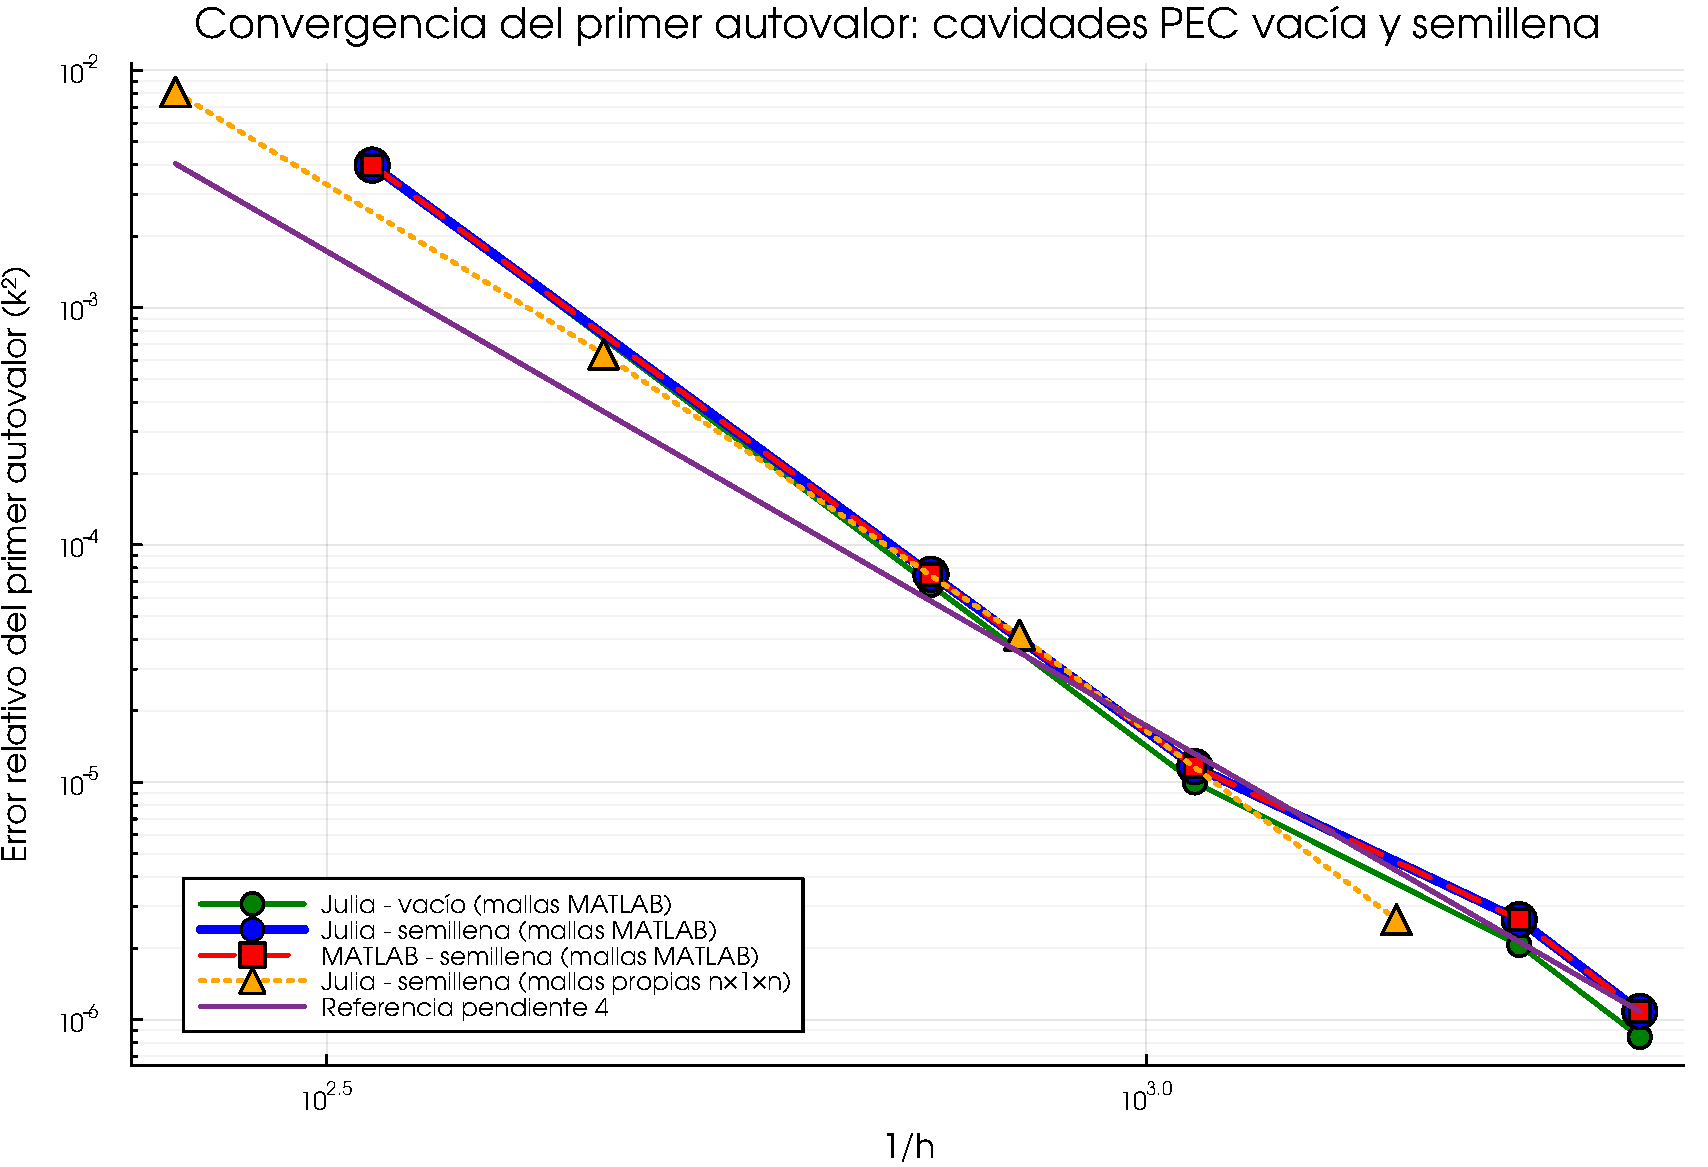
\includegraphics[width=0.85\linewidth]{convergencia_combinada_cavidades.pdf}
	\caption[Error relativo del primer modo de las cavidades vacía y semillena frente a $1/h$]{Error relativo de $\lambda_1=k^2$ de las cavidades rectangular vacía ($\varepsilon_r=1$) y semillena frente a $1/h$ (escala log-log). La semillena se calcula sobre las 5 mallas de MATLAB (curvas de Julia y MATLAB, coincidentes) y sobre nuestras mallas propias $n\times1\times n$ (curva de Julia); la vacía, sobre las mallas de MATLAB. Se incluye la línea de referencia de pendiente $4$ ($\mathrm{O}(h^4)$).}
	\label{fig:convergencia_combinada}
\end{figure}

De la figura se obtienen las pendientes log-log extremo a extremo: $4{,}76$ (vacía) y $4{,}61$ (semillena) sobre las 5 mallas exportadas en ambas implementaciones, y $4{,}68$ (semillena) sobre nuestras mallas propias $n\times1\times n$. El orden de referencia es $4$ porque el elemento es de segundo orden y, en FEM, el error de un autovalor es cuadrático en el del autovector, por lo que el error del autovalor converge a $\mathrm{O}(h^4)$.

\section{Comparación de rendimiento Julia--MATLAB}\label{sec:res-rendimiento}

Uno de los objetivos principales de la implementación en Julia de las funciones de base hexaédricas era mejorar el rendimiento de forma significativa debido a la estructura del lenguaje. MATLAB es un lenguaje interpretado que solo utiliza bibliotecas C/FORTRAN como BLAS o LAPACK para operaciones vectorizadas. Por el contrario Julia utiliza compilación JIT (Just In Time) que traduce el código a LLVM IR (Low Level Virtual Machine Intermediate Representation) de donde infiere los tipos de datos con los que se llama y aplica optimizaciones, posteriormente lo pasa a código máquina y lo almacena en caché para futuros usos \cite{juliajitdocs}. Según esto lo esperable es que Julia tenga un mayor rendimiento principalmente en las etapas en las que pueda aprovechar el uso de código ya compilado almacenado en caché como bucles sobre elementos, cálculo de puntos de cuadratura y ensamblaje de K y M.


La tabla \ref{tab:tiempos} muestra los tiempos después de la primera ejecución en la malla más fina de $23124$ grados de libertad. En Julia la primera ejecución tarda más porque hace la compilación y en MATLAB también porque guarda las bases y luego las reutiliza en lugar de calcularlas.

\begin{table}[htbp]
	\centering
	\caption{Tiempo por etapa en la malla de 23124 grados de libertad.}
	\label{tab:tiempos}
	\begin{tabular}{lrrr}
		\toprule
		\textbf{Etapa} & \textbf{Julia} & \textbf{MATLAB} & \textbf{Cociente} \\
		\midrule
		Coeficientes & 4,5 ms & 251,0 ms & 56 \\
		Numeración de DOF & 1,0 ms & 28,3 ms & 30 \\
		Ensamblaje + Dirichlet & 1199,4 ms & 17136,7 ms & 14 \\
		Resolución & 391,8 ms & 424,2 ms & 1,1 \\
		\bottomrule
	\end{tabular}
\end{table}



\begin{table}[htbp]
	\centering
	\caption{Cociente de tiempos (Julia frente a MATLAB) por etapa y malla.}
	\label{tab:tiempos-todas}
	\begin{tabular}{lrrrrr}
		\toprule
		\textbf{Etapa} & \textbf{Malla 1} & \textbf{Malla 2} & \textbf{Malla 3} & \textbf{Malla 4} & \textbf{Malla 5} \\
		\midrule
		Coeficientes & $56{,}3\times$ & $56{,}3\times$ & $56{,}3\times$ & $56{,}3\times$ & $56{,}3\times$ \\
		Numeración de DOF & $51{,}3\times$ & $40{,}8\times$ & $51{,}8\times$ & $33{,}2\times$ & $29{,}7\times$ \\
		Ensamblaje + Dirichlet & $28{,}5\times$ & $20{,}8\times$ & $20{,}4\times$ & $15{,}6\times$ & $14{,}3\times$ \\
		Resolución & $3{,}0\times$ & $0{,}16\times$ & $0{,}03\times$ & $1{,}28\times$ & $1{,}08\times$ \\
		\bottomrule
	\end{tabular}
\end{table}

Julia es entre $14$ y $56$ veces más rápida que MATLAB en lo implementado en el trabajo y tiene un rendimiento comparable en el solver de autovalores ya que ambos utilizan ARPACK. Estos resultados son coherentes con trabajos anteriores de la universidad. En el informe de \cite{nunez2023julia} (MATLAB frente a Julia) y en el de \cite{mohedano2023julia} (Julia frente a Python) realiza una comparación de integración numérica de Gauss-Legendre que da como resultados que Julia es hasta $\sim300$ veces más rápida que MATLAB y $\sim100$ veces más rápida que Python que son ambos lenguajes interpretados. Nuestro benchmark confirma el mismo resultado, si bien es cierto que con una ventaja máxima de $\sim50$, es atribuible a que utilizaban una única operación escalar en bucle donde los lenguajes interpretados sufren más. Aun así es cierto que estos resultados pueden indicar hay potencial de mejora.



\subsection{Memoria utilizada}\label{sec:res-memoria}
Como ambas implementaciones construyen el mismo problema discreto (secciones \ref{sec:res-ensamblaje} y \ref{sec:res-cavidad}), la memoria de las matrices $\mathbf{K}$ y $\mathbf{M}$ es prácticamente idéntica. La \autoref{tab:memoria} resume la memoria del bloque libre-libre (las matrices del problema resuelto) y de la matriz completa $n_{dof}\times n_{dof}$ que se construye durante el ensamblaje.

\begin{table}[htbp]
	\centering
	\caption{Memoria de $\mathbf{K}$ y $\mathbf{M}$ por malla: bloque libre-libre y matriz completa $n_{dof}\times n_{dof}$.}
	\label{tab:memoria}
	\begin{tabular}{lrrrrrrr}
		\toprule
		\textbf{Malla} & \textbf{$n_{dof}$} &
		\multicolumn{3}{c}{\textbf{Bloque libre-libre}} &
		\multicolumn{3}{c}{\textbf{Matriz completa}} \\
		\cmidrule(lr){3-5} \cmidrule(lr){6-8}
		& & \textbf{Julia} & \textbf{MATLAB} & \textbf{Coc.} &
		\textbf{Julia} & \textbf{MATLAB} & \textbf{Coc.} \\
		\midrule
		1 & 318 & 61,4 KB & 59,9 KB & 1,03 & 144,4 KB & 70,4 KB & 2,05 \\
		2 & 1678 & 664,6 KB & 662,4 KB & 1,00 & 1,3 MB & 708,9 KB & 1,89 \\
		3 & 4062 & 1,8 MB & 1,8 MB & 1,00 & 3,6 MB & 1,9 MB & 1,87 \\
		4 & 14916 & 15,8 MB & 15,8 MB & 1,00 & 26,8 MB & 28,2 MB & 0,95 \\
		5 & 23124 & 25,2 MB & 25,2 MB & 1,00 & 46,5 MB & 44,3 MB & 1,05 \\
		\bottomrule
	\end{tabular}
\end{table}

La memoria crece conforme aumenta $n_{dof}$, lo que era de esperar. En el bloque libre-libre (las matrices del problema a resolver) coinciden. Para la matriz completa $n_{dof}\times n_{dof}$  Julia es mayor para mallas pequeñas debido al coste fijo de la representación dispersa. También es destacable que al ejecutar ambas al mismo tiempo Julia consume algo más de RAM al cargar las ejecuciones JIT en la caché.

%--------------------------------------------------------------------------
\chapter{Discusión y conclusiones}\label{cap:conclusiones}
%--------------------------------------------------------------------------

\section{Discusión de los resultados}\label{sec:discusion}
\subsection{Validación de las funciones de base hexaédricas}
Han sido validadas de diferentes maneras independientes: la matriz de coeficientes $W$ coincide entrada a entrada con la Tabla II del artículo, se cumple la propiedad dual $g_i(N_j)=\delta_{ij}$, se obtienen los números de acondicionamiento esperados $\kappa(M^p)=18{,}75$ y $\kappa(K^p)=35{,}12$ y se resuelve un problema de autovalores que utiliza esas funciones de base para obtener resultados numéricos que coinciden con los analíticos con una tasa de convergencia $4{,}61$ y una tasa de error absoluto de $10^{-5}$ para mallas finas.

\subsection{Rendimiento}
Como se expuso en \ref{sec:res-rendimiento}, Julia tiene un rendimiento de entre $14$ y $56$ veces superior según la etapa, exceptuando el solver. Si bien es un buen resultado, el perfilado del ensamblaje con el módulo estándar \texttt{Profile} de Julia (perfil de muestreo de CPU y perfil de asignaciones \texttt{Profile.Allocs}) indica que aún hay margen de mejora.

\begin{table}[htbp]
	\centering
	\caption{Salida del Profiler sobre el ensamblaje. \texttt{Count} es el número de muestras de CPU (malla 3, 4062 DOF, 10 llamadas, 3890 muestras en total); \texttt{Allocs} son las asignaciones de memoria en una sola llamada (malla 1, 318 DOF).}
	\label{tab:perfil}
	\begin{tabular}{rrll}
		\toprule
		\texttt{Count} & \texttt{Allocs} & \texttt{File} & \texttt{Function} \\
		\midrule
		$823$ & $926\,808$ & \texttt{Assembly.jl:36} & \texttt{stiff\_matrix\_element} \\
		$589$ & $915\,800$ & \texttt{Assembly.jl:22} & \texttt{mass\_matrix\_element} \\
		$108$ & $165\,920$ & \texttt{BasisEval.jl:32} & \texttt{eval\_curl\_bases\_ref} \\
		$66$ & $168\,352$ & \texttt{BasisEval.jl:22} & \texttt{eval\_bases\_ref} \\
		$44$ & $\sim$170\,000 & \texttt{BasisEval.jl:52} & \texttt{compute\_jacobian} \\
		\bottomrule
	\end{tabular} 
\end{table}
Se puede ver que lo que ocupa la mayor cantidad de procesamiento del CPU es el cálculo de las diferentes matrices $M^e$ y $K^e$, que ocupan el $\sim36$\,\% del tiempo total. Al observar el perfil de asignaciones se puede ver que en cada uno de los 27 puntos de Gauss del elemento se reevalúan en las funciones de base del elemento de referencia, se recalcula el Jacobiano y se ejecutan $N N^\top$ y $W^\top M$, lo que genera más de $900\,000$ asignaciones en el ensamblaje. Aunque este enfoque es el que usa MATLAB y es más general, se pueden realizar diferentes optimizaciones como precalcular las funciones de base evaluadas en los puntos de referencia, también se puede reutilizar el Jacobiano al ser una malla regular y se puede aprovechar que producto  $N N^\top$, da una matriz simétrica, y utilizar syrk! para ahorrar memoria.


\section{Conclusiones}\label{sec:conclusiones}
\subsection{Conclusiones por objetivo}
Al principio del trabajo en \autoref{sec:objetivos} se definieron los siguientes objetivos.

\begin{itemize}
	\item \textbf{O1 (implementar las funciones de base).} Se han implementado en Julia las funciones de base del elemento hexaédrico curl-conforme de Nédélec de segundo orden y los módulos necesarios para evaluarlas, ensamblarlas y compararlas con una solución analítica.

	\item \textbf{O2 (obtención de los coeficientes).} Fue el primer objetivo durante la realización del trabajo, ya que era el primer momento en el que se podía comprobar la corrección de la implementación: se obtuvieron los mismos resultados de la Tabla II del artículo.

	\item \textbf{O3 (verificar el ensamblaje global).} Se implementa la integración numérica de Gauss para 1D, 2D y 3D y los tres tipos de funcionales, y por último se comprueba que las matrices $\mathbf{K}$ y $\mathbf{M}$ tienen la dimensión del núcleo correcta y coinciden con las de MATLAB.

	\item \textbf{O4 (reproducir el benchmark de la cavidad).} El objetivo era comprobar que las funciones de base producen autovalores que coinciden con la solución analítica y con MATLAB, y que la convergencia reproduce la tasa del artículo (sección \ref{sec:res-cavidad}). Además se pueden implementar diferentes mallas y topologías.

	\item \textbf{O5 (comparar el rendimiento).} En el benchmark, Julia es entre $14$ y $56$ veces más rápida al generar los coeficientes y al ensamblar (sección \ref{sec:res-rendimiento}).
\end{itemize}

\subsection{Objetivos parcialmente cumplidos}
En general todos los objetivos se han cumplido, si bien es cierto que en la comparación de rendimiento existen mejoras aplicables. Otro de los objetivos era también que el código sea más entendible que el de referencia o que el que podría crearse equivalentemente en Fortran. Considero que se ha cumplido, sin embargo, el paquete \texttt{NedelecHex} podría simplificarse más o mejorar la documentación.

\section{Limitaciones y líneas futuras}\label{sec:limitaciones}
\subsection{Geometrías limitadas}

Solo se implementan hexaedros regulares y mallas estructuradas. Se podría expandir la implementación en Julia al resto de las familias ya implementadas en HOFEM, tetraedros y prismas triangulares, o ampliar la implementación a hexaedros distorsionados.

\subsection{Ampliar las topologías y condiciones de contorno}
El paquete \texttt{NedelecHex} incluye únicamente las funciones necesarias para resolver el problema de la cavidad semillena rodeada de un conductor perfecto. Al utilizar etiquetas en las mallas, bastaría con funciones que apliquen otras condiciones de contorno (Neumann, Robin) y otras topologías (PEC en el centro, varios dieléctricos\ldots).

\subsection{Mejoras de rendimiento}
Se podrían aplicar las mejoras de \autoref{sec:res-rendimiento} para quitar la carga del cálculo de las matrices de masa y rigidez elementales.



%--------------------------------------------------------------------------
\chapter{Marco regulador}\label{cap:marco-regulador}
%--------------------------------------------------------------------------

\section{Reglamento General de Protección de Datos}
El RGPD (Reglamento (UE) 2016/679) se aplica debido a que el presente trabajo es un software de método de elementos finitos sin entradas, tratamiento ni salidas de datos personales en ninguna fase del proyecto.

\section{Estándares técnicos}\label{sec:estandares}
El trabajo utiliza los siguientes estándares: el formato de malla de Gmsh, \cite{geuzaine2009gmsh} para representar y etiquetar las mallas, la aritmética IEEE 754, por la que se puede describir los umbrales de tolerancia de ($10^{-13}$--$10^{-15}$) como error de máquina, la guía de estilo de Julia y el estilo de citación IEEE.

\section{Propiedad intelectual e industrial}\label{sec:propiedad}
El lenguaje Julia se distribuye bajo la licencia MIT que permite reutilizar el software dentro de software propietario mientras se conserven los términos de la licencia y el aviso de copyright. De manera parecida Gmsh \cite{geuzaine2009gmsh} utiliza  la licencia GNU General Public License (GPL) aunque al utilizarlo como herramienta externa NedelecHex no queda obligado a ser GPL.

La implementación de Adrian Amor de MATLAB \cite{amor2022zenodo} se publica en Zenodo como código con licencia (``Other (Open)''), es decir, Open Source sin especificar una licencia concreta. MATLAB es software propietario y comercial de MathWorks, que utiliza una licencia de pago.

El código desarrollado en este TFG y la propia memoria se publican bajo la Licencia Creative Commons que se indica en la portada que permite su difusión y consulta.

%--------------------------------------------------------------------------
\chapter{Entorno socio-económico}\label{cap:entorno}
%--------------------------------------------------------------------------

\section{Presupuesto}\label{sec:presupuesto}
El principal coste sería el trabajo del estudiante. Se toma la estimación de 12 créditos x 25 horas al salario mínimo, por elegir un valor. Julia, Gmsh, git, TeXstudio y el resto de las licencias utilizadas son gratuitas exceptuando el uso de la API de Deepseek y la licencia de MATLAB que proporciona la universidad.

\begin{table}[htbp]
	\centering
	\caption{Presupuesto del TFG.}
	\label{tab:presupuesto}
	\begin{tabular}{@{}p{5.4cm}r@{\hspace{0.6cm}}p{6.2cm}@{}}
		\toprule
		Concepto & Importe (\euro) & Notas \\
		\midrule
		Personal (300 h $\times$ 9,26\,\euro/h) & 2778,00 & 12 ECTS $\times$ 25 h al SMI \\
		Licencias de software & 8,00 & API DeepSeek \\
		\midrule
		\textbf{Total} & \textbf{2786,00} & \\
		\midrule
		Licencia MATLAB académica & 316,00 &  \\
		\bottomrule
	\end{tabular}
\end{table}

\section{Impacto socio-económico}\label{sec:impacto}
El software de este trabajo puede tener un impacto positivo al ser una alternativa gratuita al eliminar la barrera del código propietario de MATLAB ya que la implementación de referencia utilizaba librerías no disponibles en Octave. Aunque en este trabajo en concreto no es tan relevante si se escalara en algún momento la mejora de rendimiento de Julia sobre MATLAB podría incurrir en beneficios respecto al consumo energético  o la capacidad de ejecución de análisis de elementos finitos en dispositivos de menor capacidad.


%==========================================================================
%	BIBLIOGRAFÍA
%==========================================================================
% Recoge solo las fuentes citadas en el cuerpo del trabajo. Con estilo IEEE
% se ordenan por orden de aparición en el texto; con APA, alfabéticamente.
%==========================================================================


\clearpage
\phantomsection
\addcontentsline{toc}{chapter}{Bibliografía}
\setquotestyle[english]{british} % en el estilo IEEE se usan las comillas inglesas
\printbibliography


%==========================================================================
%	ANEXOS
%==========================================================================
%	ANEXOS
%==========================================================================
\clearpage

\phantomsection
\chapter*{Anexo A. Salida de la suite de tests}
\addcontentsline{toc}{chapter}{Anexo A. Salida de la suite de tests}

Este anexo reproduce, de forma íntegra y sin resumir, la salida que produce la suite de tests del paquete \texttt{NedelecHex} al ejecutar \texttt{julia --project=. test/runtests.jl}. La suite consta de 11 ficheros (\texttt{test\_01} a \texttt{test\_11}) y ejecuta en total \textbf{1498 comprobaciones, todas superadas}. El análisis y la discusión de estos resultados se encuentran en el capítulo \ref{cap:resultados}; aquí se documenta la salida cruda para su reproducibilidad.

\begin{lstlisting}[numbers=none, captionpos=b, caption={Salida completa de la suite de tests.}, label=cod:salida-tests]
Test Summary:                           | Pass  Total  Time
GaussQuadrature.jl: Cuadratura de Gauss |   17     17  0.9s
Test Summary:                                   | Pass  Total  Time
Monomials.jl: Los 54 monomios vectoriales de H2 |  380    380  0.4s
Test Summary:                          | Pass  Total  Time
DOFs.jl: Integrales de DOF tipo arista |    4      4  0.5s
Test Summary:                        | Pass  Total  Time
DOFs.jl: Integrales de DOF tipo cara |    4      4  0.2s
Test Summary:                           | Pass  Total  Time
DOFs.jl: Integrales de DOF tipo volumen |    4      4  0.3s
Test Summary:                              | Pass  Total  Time
CoefficientGenerator.jl: Matriz G completa |    3      3  0.5s
Test Summary:                                                 | Pass  Total  Time
CoefficientGenerator.jl: Coeficientes W vs Tabla II del paper |    5      5  1.8s
Test Summary:                                      | Pass  Total  Time
BasisEval.jl: Jacobiano del elemento de referencia |   18     18  0.7s
Test Summary:                                  | Pass  Total  Time
BasisEval.jl: Propiedad dual de la base y curl |   11     11  2.0s
Test Summary:                                                     | Pass  Total  Time
Assembly.jl: Matrices locales Ke, Me en el elemento de referencia |    8      8  1.3s
Test Summary:                                  | Pass  Total  Time
Mesh.jl: Permutacion de orden de nodos de Gmsh |   30     30  1.6s
Test Summary:                                                                                 | Pass  Total  Time
BasisEval.jl: Evaluacion de las 54 bases vs MATLAB (equivalente a mainEvaluateCoefficients.m) |    5      5  2.2s
Test Summary:        | Pass  Total  Time
Assembly: 1 elemento |    5      5  0.9s
Test Summary:                                       | Pass  Total  Time
Assembly: 2 elementos adyacentes (DOFs compartidos) |  155    155  0.4s
Test Summary:         | Pass  Total  Time
Assembly: malla 2x2x2 |    9      9  0.5s
Test Summary:                                             | Pass  Total  Time
Assembly: dimension del nucleo de K en mallas adicionales |    3      3  0.6s

-- malla 1 --
  n_free   MATLAB=94  Julia=94
  ||Kf||_F MATLAB=1.368220e+06  Julia=1.368220e+06  difrel=9.02e-15
  ||Mf||_F MATLAB=5.403556e-01  Julia=5.403556e-01  difrel=1.38e-14
  tr(Kf)   MATLAB=6.583296e+06  Julia=6.583296e+06  difrel=7.21e-15
  tr(Mf)   MATLAB=2.627840e+00  Julia=2.627840e+00  difrel=2.59e-14

-- malla 2 --
  n_free   MATLAB=686  Julia=686
  ||Kf||_F MATLAB=2.993986e+06  Julia=2.993986e+06  difrel=2.33e-15
  ||Mf||_F MATLAB=2.720014e-01  Julia=2.720014e-01  difrel=1.18e-14
  tr(Kf)   MATLAB=4.356398e+07  Julia=4.356398e+07  difrel=1.88e-15
  tr(Mf)   MATLAB=4.499982e+00  Julia=4.499982e+00  difrel=1.14e-14

-- malla 3 --
  n_free   MATLAB=1790  Julia=1790
  ||Kf||_F MATLAB=5.989873e+06  Julia=5.989873e+06  difrel=9.33e-16
  ||Mf||_F MATLAB=2.769618e-01  Julia=2.769618e-01  difrel=1.86e-14
  tr(Kf)   MATLAB=1.413001e+08  Julia=1.413001e+08  difrel=3.16e-15
  tr(Mf)   MATLAB=7.561984e+00  Julia=7.561984e+00  difrel=1.16e-14

-- malla 4 --
  n_free   MATLAB=9796  Julia=9796
  ||Kf||_F MATLAB=2.153904e+07  Julia=2.153904e+07  difrel=4.84e-15
  ||Mf||_F MATLAB=3.658779e-01  Julia=3.658779e-01  difrel=8.80e-15
  tr(Kf)   MATLAB=1.115996e+09  Julia=1.115996e+09  difrel=1.86e-14
  tr(Mf)   MATLAB=2.197040e+01  Julia=2.197040e+01  difrel=1.92e-14

-- malla 5 --
  n_free   MATLAB=15444  Julia=15444
  ||Kf||_F MATLAB=3.055003e+07  Julia=3.055003e+07  difrel=3.41e-15
  ||Mf||_F MATLAB=3.747734e-01  Julia=3.747734e-01  difrel=1.17e-14
  tr(Kf)   MATLAB=1.993523e+09  Julia=1.993523e+09  difrel=1.87e-14
  tr(Mf)   MATLAB=2.874112e+01  Julia=2.874112e+01  difrel=1.62e-14
Test Summary:                                        | Pass  Total  Time
Assembly: comparacion K/M globales MATLAB vs Julia ( |   25     25  7.4s
Test Summary:                                        | Pass  Total  Time
Etiquetas: box_mesh trae el contorno puesto por Gmsh |    5      5  0.1s
Test Summary:                                                       | Pass  Total  Time
Etiquetas: el Dirichlet por etiqueta = el geometrico (no regresion) |    5      5  0.0s
Test Summary:                                    | Pass  Total  Time
Etiquetas: sin etiquetas no se adivina, se falla |    2      2  0.1s
Test Summary:                                                        | Pass  Total  Time
Etiquetas: PEC parcial (lo que el criterio geometrico no sabe hacer) |    2      2  0.3s
Test Summary:                                     | Pass  Total  Time
Etiquetas: material por solido y el eje del corte |    4      4  0.5s
  malla 1: 8 elem, criterio en x acierta 8, en z 4
  malla 2: 48 elem, criterio en x acierta 48, en z 24
  malla 3: 120 elem, criterio en x acierta 120, en z 60
  malla 4: 512 elem, criterio en x acierta 512, en z 256
  malla 5: 800 elem, criterio en x acierta 800, en z 400
Test Summary:                                            | Pass  Total  Time
Etiquetas: las mallas de MATLAB traen su propio material |   20     20  0.3s
k101   =   353.7838 rad/m
k201   =   544.5049 rad/m
k102   =   599.7987 rad/m
k301   =   750.3145 rad/m
k202   =   763.3160 rad/m
k103   =   809.5754 rad/m
Test Summary:                                                       | Pass  Total  Time
HalfFilledCavity.jl: Autovalores analiticos de la cavidad semillena |   21     21  0.4s
k101    fem=  355.214  analitico=  353.784  err=0.4%
k201    fem=  548.071  analitico=  544.505  err=0.7%
k102    fem=  611.475  analitico=  599.799  err=1.9%
k301    fem=  789.109  analitico=  750.314  err=5.2%
k202    fem=  880.110  analitico=  763.316  err=15.3%
k103    fem=  986.483  analitico=  809.575  err=21.9%
Test Summary:                                                | Pass  Total  Time
HalfFilledCavity.jl: Autovalores FEM en malla gruesa (2x2x2) |    9      9  0.8s
Warning: El elemento 1 cruza el plano z = 0.005 (rango [0.0, 0.01]): el corte no cae en una capa de la malla y el material es ambiguo.
  @ NedelecHex.Mesh ~/TFG-FEM/NedelecHex/src/Geometry/Mesh.jl:170

n         h             error rel. k2
1         1.0000        5.979e-01
2         0.5000        8.104e-03
4         0.2500        6.360e-04
8         0.1250        4.168e-05

Pendiente log-log (extremo a extremo, como el paper): 4.60  (paper: 4.55, Fig. 7)
Pendiente log-log (minimos cuadrados n=2,4,8): 3.80
Test Summary:                                                | Pass  Total  Time
HalfFilledCavity.jl: Convergencia O(h4) del primer autovalor |    2      2  1.2s

malla     n_free    err_medio   tiempo
------------------------------------------
1         94        6.75e-02    0.0s
2         686       2.07e-03    0.1s
3         1790      3.32e-04    0.6s
4         9796      7.53e-05    3.0s
5         15444     3.10e-05    3.0s
Test Summary:                                                             | Pass  Total   Time
HalfFilledCavity.jl: Equivalencia con mainHalfFilled.m (mallas de MATLAB) |   26     26  10.1s

malla     n_dofs      ||x_fem - x_exacto|| / ||x_exacto||
1         54          1.454e-15
2         300         3.984e-14
3         882         1.504e-13
Test Summary:                                                   | Pass  Total  Time
MMS - Exactitud en H2 (Metodo de las Soluciones Manufacturadas) |  711    711  2.4s

n         h             error (campo)     error_curl
1         1.0000        5.004e-02     6.945e-02
2         0.5000        1.244e-02     1.752e-02
4         0.2500        3.107e-03     4.389e-03
8         0.1250        7.765e-04     1.098e-03

Pendiente log-log: error=2.00  error_curl=1.99  (esperada entre 2 y 3)
Test Summary:                                   | Pass  Total   Time
MMS - Tasa de convergencia (onda plana oblicua) |    5      5  10.8s
\end{lstlisting}

%--------------------------------------------------------------------------
% ANEXO B: matrices de coeficientes W (Julia y MATLAB) sin redondear
%--------------------------------------------------------------------------
\clearpage
\begin{landscape}
\phantomsection
\chapter*{Anexo B. Matrices de coeficientes $W$}
\addcontentsline{toc}{chapter}{Anexo B. Matrices de coeficientes $W$}

\subsection*{Matriz $W$ obtenida con Julia}
\begin{lstlisting}[numbers=none, basicstyle=\ttfamily\tiny, captionpos=b, caption={Matriz de coeficientes $W = G^{-1}$ ($54\times54$) calculada con Julia, sin redondear.}, label=cod:W-julia]
4.000000000000008	-2.0000000000000013	0.0	0.0	1.6875389974302408e-14	4.6629367034256646e-15	0.0	0.0	-1.0658141036401498e-14	-2.1304974245700415e-15	0.0	0.0	-9.975045480972425e-15	-6.9661354873818425e-15	0.0	0.0	0.0	0.0	0.0	0.0	0.0	0.0	0.0	0.0	-4.263256414560609e-14	-1.6875389974302408e-14	0.0	0.0	2.939109860838695e-14	-1.3601260035940234e-14	0.0	0.0	-6.267620167721787e-15	3.103792942824751e-14	0.0	0.0	0.0	0.0	0.0	0.0	-4.307768133973818e-14	-1.1183441004534346e-14	0.0	0.0	0.0	0.0	0.0	0.0	-5.484501741648268e-14	1.2860083368574769e-14	0.0	0.0	0.0	0.0
-6.000000000000017	6.000000000000004	0.0	0.0	-2.664535259100382e-14	-6.661338147750955e-15	0.0	0.0	1.3322676295501877e-14	4.63209717496386e-15	0.0	0.0	1.3526217183349847e-14	1.0553286639631378e-14	0.0	0.0	0.0	0.0	0.0	0.0	0.0	0.0	0.0	0.0	6.927791673660993e-14	2.3980817331903438e-14	0.0	0.0	-4.254621346591303e-14	1.7529187977692768e-14	0.0	0.0	1.0941864698250083e-14	-4.80973285890387e-14	0.0	0.0	0.0	0.0	0.0	0.0	6.61569564562747e-14	1.4568593245359025e-14	0.0	0.0	0.0	0.0	0.0	0.0	8.260059303211161e-14	-1.6209256159527355e-14	0.0	0.0	0.0	0.0
-16.000000000000032	8.000000000000025	0.0	0.0	-8.000000000000032	3.9999999999999787	0.0	0.0	8.881784197001218e-15	8.417135301510033e-15	0.0	0.0	3.033376019503624e-14	7.035524426420935e-15	0.0	0.0	0.0	0.0	0.0	0.0	0.0	0.0	0.0	0.0	24.00000000000008	-12.000000000000009	0.0	0.0	-6.833217119711432e-14	3.1226050551864586e-14	0.0	0.0	4.282171325350524e-14	-5.959841673672978e-14	0.0	0.0	0.0	0.0	0.0	0.0	9.828352123922426e-14	3.7245926507609886e-14	0.0	0.0	0.0	0.0	0.0	0.0	9.76996261670136e-14	-3.922788020342213e-14	0.0	0.0	0.0	0.0
24.000000000000107	-24.000000000000078	-0.0	-0.0	12.000000000000082	-11.999999999999988	-0.0	-0.0	1.0658141036401528e-14	-4.085312335335967e-14	-0.0	-0.0	-2.1270022780110345e-14	-2.6790298374774325e-14	-0.0	-0.0	-0.0	-0.0	-0.0	-0.0	-0.0	-0.0	-0.0	-0.0	-36.000000000000206	36.000000000000085	-0.0	-0.0	5.004021888213288e-14	-1.0368249468860521e-14	-0.0	-0.0	-1.5266183379165173e-13	1.4585246590728408e-13	-0.0	-0.0	-0.0	-0.0	-0.0	-0.0	-2.0388012266102573e-13	-7.407654736526766e-15	-0.0	-0.0	-0.0	-0.0	-0.0	-0.0	1.332267629550191e-14	-7.005507285384752e-14	-0.0	-0.0	-0.0	-0.0
12.000000000000018	-6.00000000000002	0.0	0.0	12.000000000000023	-5.999999999999989	0.0	0.0	1.3322676295502295e-15	-5.057682667736884e-15	0.0	0.0	-2.1242267204494584e-14	1.2335811384719086e-16	0.0	0.0	0.0	0.0	0.0	0.0	0.0	0.0	0.0	0.0	-24.000000000000036	12.000000000000023	0.0	0.0	4.0806864060666687e-14	-1.8898463041396987e-14	0.0	0.0	-4.006671537758372e-14	2.7040098555315137e-14	0.0	0.0	0.0	0.0	0.0	0.0	-5.0872886150601826e-14	-2.7484187765164818e-14	0.0	0.0	0.0	0.0	0.0	0.0	-4.796163466380644e-14	3.2862601528904223e-14	0.0	0.0	0.0	0.0
-18.00000000000008	18.000000000000068	-0.0	-0.0	-18.00000000000007	18.000000000000007	-0.0	-0.0	-2.5979218776228707e-14	3.581394440269994e-14	-0.0	-0.0	7.632783294297847e-15	1.6051974564372132e-14	-0.0	-0.0	-0.0	-0.0	-0.0	-0.0	-0.0	-0.0	-0.0	-0.0	36.000000000000135	-36.00000000000011	-0.0	-0.0	-8.752258177461415e-15	-8.123131796840893e-15	-0.0	-0.0	1.4852933697776946e-13	-9.701498863516208e-14	-0.0	-0.0	-0.0	-0.0	-0.0	-0.0	1.3276417002809206e-13	-7.234953377140845e-15	-0.0	-0.0	-0.0	-0.0	-0.0	-0.0	-8.792966355031269e-14	7.960299086562439e-14	-0.0	-0.0	-0.0	-0.0
-15.999999999999961	8.000000000000002	0.0	0.0	4.085620730620591e-14	-4.426089124838988e-14	0.0	0.0	-7.9999999999999645	4.000000000000003	0.0	0.0	4.6185277824406645e-14	-2.2278475360811603e-14	0.0	0.0	0.0	0.0	0.0	0.0	0.0	0.0	0.0	0.0	-8.245256329549598e-14	9.459100169806415e-14	0.0	0.0	-1.0672944010063217e-13	8.718951486722929e-14	0.0	0.0	23.99999999999998	-12.000000000000044	0.0	0.0	0.0	0.0	0.0	0.0	-5.6695389124191815e-14	8.985405012632977e-14	0.0	0.0	0.0	0.0	0.0	0.0	2.596441580256714e-13	-1.5010215292932207e-13	0.0	0.0	0.0	0.0
23.999999999999957	-24.000000000000007	-0.0	-0.0	-6.128431095930879e-14	6.539213615042214e-14	-0.0	-0.0	11.999999999999964	-12.000000000000004	-0.0	-0.0	-6.927791673660993e-14	3.341771304121736e-14	-0.0	-0.0	-0.0	-0.0	-0.0	-0.0	-0.0	-0.0	-0.0	-0.0	1.236788449432438e-13	-1.3788969965844558e-13	-0.0	-0.0	1.5210055437364705e-13	-1.3078427230084387e-13	-0.0	-0.0	-36.00000000000001	36.00000000000007	-0.0	-0.0	-0.0	-0.0	-0.0	-0.0	8.104628079763698e-14	-1.30784272300844e-13	-0.0	-0.0	-0.0	-0.0	-0.0	-0.0	-3.894662370385069e-13	2.331468351712841e-13	-0.0	-0.0	-0.0	-0.0
64.00000000000003	-32.000000000000185	0.0	0.0	31.99999999999988	-15.999999999999943	0.0	0.0	31.999999999999826	-15.999999999999979	0.0	0.0	15.99999999999982	-7.999999999999883	0.0	0.0	0.0	0.0	0.0	0.0	0.0	0.0	0.0	0.0	-95.9999999999999	48.0000000000001	0.0	0.0	-47.999999999999616	23.999999999999783	0.0	0.0	-95.9999999999999	48.00000000000015	0.0	0.0	0.0	0.0	0.0	0.0	-47.99999999999966	23.999999999999766	0.0	0.0	0.0	0.0	0.0	0.0	143.99999999999932	-71.99999999999973	0.0	0.0	0.0	0.0
-96.0000000000005	96.0000000000005	-0.0	-0.0	-48.000000000000156	48.000000000000114	-0.0	-0.0	-48.00000000000005	48.0000000000001	-0.0	-0.0	-24.00000000000001	23.999999999999975	-0.0	-0.0	-0.0	-0.0	-0.0	-0.0	-0.0	-0.0	-0.0	-0.0	144.0000000000007	-144.0000000000006	-0.0	-0.0	72.00000000000004	-72.00000000000001	-0.0	-0.0	144.0000000000006	-144.00000000000057	-0.0	-0.0	-0.0	-0.0	-0.0	-0.0	72.00000000000014	-72.00000000000004	-0.0	-0.0	-0.0	-0.0	-0.0	-0.0	-216.0000000000006	216.00000000000043	-0.0	-0.0	-0.0	-0.0
-48.000000000000064	24.000000000000178	-0.0	-0.0	-47.999999999999936	24.000000000000007	-0.0	-0.0	-23.999999999999826	11.999999999999948	-0.0	-0.0	-23.999999999999844	11.9999999999999	-0.0	-0.0	-0.0	-0.0	-0.0	-0.0	-0.0	-0.0	-0.0	-0.0	96.0	-48.000000000000185	-0.0	-0.0	47.99999999999966	-23.99999999999981	-0.0	-0.0	71.99999999999987	-36.00000000000008	-0.0	-0.0	-0.0	-0.0	-0.0	-0.0	71.99999999999972	-35.99999999999985	-0.0	-0.0	-0.0	-0.0	-0.0	-0.0	-143.99999999999946	71.99999999999979	-0.0	-0.0	-0.0	-0.0
72.00000000000054	-72.00000000000048	0.0	0.0	72.00000000000028	-72.00000000000023	0.0	0.0	36.00000000000005	-36.00000000000007	0.0	0.0	36.00000000000007	-36.00000000000002	0.0	0.0	0.0	0.0	0.0	0.0	0.0	0.0	0.0	0.0	-144.0000000000009	144.00000000000074	0.0	0.0	-72.00000000000013	72.00000000000006	0.0	0.0	-108.00000000000057	108.0000000000005	0.0	0.0	0.0	0.0	0.0	0.0	-108.00000000000031	108.0000000000002	0.0	0.0	0.0	0.0	0.0	0.0	216.00000000000082	-216.00000000000054	0.0	0.0	0.0	0.0
11.999999999999954	-5.999999999999999	0.0	0.0	-5.861977570020839e-14	3.9301895071730624e-14	0.0	0.0	11.999999999999982	-6.000000000000007	0.0	0.0	-3.730349362740534e-14	3.064215547965439e-14	0.0	0.0	0.0	0.0	0.0	0.0	0.0	0.0	0.0	0.0	1.1723955140041678e-13	-7.727152251391106e-14	0.0	0.0	7.993605777301145e-14	-7.460698725481068e-14	0.0	0.0	-23.999999999999964	12.00000000000002	0.0	0.0	0.0	0.0	0.0	0.0	9.858780458671413e-14	-7.993605777301145e-14	0.0	0.0	0.0	0.0	0.0	0.0	-2.1316282072803054e-13	1.438849039914206e-13	0.0	0.0	0.0	0.0
-17.999999999999943	18.0	-0.0	-0.0	8.792966355031252e-14	-5.795364188543325e-14	-0.0	-0.0	-17.999999999999993	18.000000000000014	-0.0	-0.0	5.5955240441107965e-14	-4.5963233219481544e-14	-0.0	-0.0	-0.0	-0.0	-0.0	-0.0	-0.0	-0.0	-0.0	-0.0	-1.7585932710062505e-13	1.1191048088221593e-13	-0.0	-0.0	-1.1191048088221593e-13	1.1191048088221593e-13	-0.0	-0.0	35.999999999999986	-36.000000000000036	-0.0	-0.0	-0.0	-0.0	-0.0	-0.0	-1.438849039914205e-13	1.159072837708665e-13	-0.0	-0.0	-0.0	-0.0	-0.0	-0.0	3.1974423109204554e-13	-2.2382096176443186e-13	-0.0	-0.0	-0.0	-0.0
-47.99999999999999	24.000000000000135	-0.0	-0.0	-23.999999999999858	11.999999999999943	-0.0	-0.0	-47.99999999999982	23.999999999999982	-0.0	-0.0	-23.99999999999982	11.999999999999888	-0.0	-0.0	-0.0	-0.0	-0.0	-0.0	-0.0	-0.0	-0.0	-0.0	71.99999999999987	-36.00000000000004	-0.0	-0.0	71.99999999999964	-35.99999999999981	-0.0	-0.0	95.99999999999983	-48.00000000000012	-0.0	-0.0	-0.0	-0.0	-0.0	-0.0	47.999999999999616	-23.99999999999977	-0.0	-0.0	-0.0	-0.0	-0.0	-0.0	-143.99999999999932	71.99999999999972	-0.0	-0.0	-0.0	-0.0
72.00000000000043	-72.00000000000041	0.0	0.0	36.00000000000013	-36.00000000000011	0.0	0.0	72.00000000000006	-72.00000000000011	0.0	0.0	36.000000000000014	-35.99999999999999	0.0	0.0	0.0	0.0	0.0	0.0	0.0	0.0	0.0	0.0	-108.00000000000063	108.0000000000005	0.0	0.0	-108.00000000000011	108.00000000000006	0.0	0.0	-144.0000000000005	144.00000000000054	0.0	0.0	0.0	0.0	0.0	0.0	-72.00000000000011	72.00000000000004	0.0	0.0	0.0	0.0	0.0	0.0	216.00000000000057	-216.0000000000004	0.0	0.0	0.0	0.0
36.00000000000004	-18.00000000000014	-0.0	-0.0	35.999999999999915	-17.999999999999993	-0.0	-0.0	35.99999999999981	-17.999999999999947	-0.0	-0.0	35.999999999999844	-17.999999999999915	-0.0	-0.0	-0.0	-0.0	-0.0	-0.0	-0.0	-0.0	-0.0	-0.0	-71.99999999999999	36.00000000000012	-0.0	-0.0	-71.99999999999967	35.99999999999983	-0.0	-0.0	-71.99999999999982	36.00000000000005	-0.0	-0.0	-0.0	-0.0	-0.0	-0.0	-71.99999999999969	35.999999999999844	-0.0	-0.0	-0.0	-0.0	-0.0	-0.0	143.99999999999943	-71.99999999999976	-0.0	-0.0	-0.0	-0.0
-54.0000000000005	54.000000000000426	0.0	0.0	-54.00000000000025	54.0000000000002	0.0	0.0	-54.000000000000036	54.00000000000007	0.0	0.0	-54.000000000000085	54.00000000000005	0.0	0.0	0.0	0.0	0.0	0.0	0.0	0.0	0.0	0.0	108.00000000000084	-108.00000000000064	0.0	0.0	108.00000000000018	-108.0000000000001	0.0	0.0	108.0000000000005	-108.00000000000045	0.0	0.0	0.0	0.0	0.0	0.0	108.00000000000028	-108.00000000000018	0.0	0.0	0.0	0.0	0.0	0.0	-216.0000000000008	216.0000000000005	0.0	0.0	0.0	0.0
0.0	0.0	-1.6875389974302376e-14	8.88178419700125e-16	0.0	0.0	4.000000000000004	-1.9999999999999911	0.0	0.0	-6.938893903906783e-17	-1.3697376566312872e-14	0.0	0.0	-2.289834988289369e-15	5.134781488891285e-16	0.0	0.0	0.0	0.0	0.0	0.0	0.0	0.0	0.0	0.0	-3.5527136788005e-15	2.5757174171303625e-14	0.0	0.0	2.944866572818226e-14	-1.0269562977782601e-15	0.0	0.0	0.0	0.0	4.579669976578757e-15	-1.0269562977782633e-15	0.0	0.0	0.0	0.0	0.0	0.0	8.88178419700125e-14	-2.944866572818226e-14	0.0	0.0	0.0	0.0	-1.2945200467129323e-13	9.159339953157515e-15	0.0	0.0
-0.0	-0.0	-8.000000000000014	4.000000000000069	-0.0	-0.0	-16.000000000000057	8.00000000000003	-0.0	-0.0	-8.39863158443301e-16	3.995260912227474e-14	-0.0	-0.0	-4.521588864642364e-14	1.7813939623823473e-14	-0.0	-0.0	-0.0	-0.0	-0.0	-0.0	-0.0	-0.0	-0.0	-0.0	24.000000000000185	-12.000000000000227	-0.0	-0.0	4.3522798533870284e-14	-2.043015962166702e-14	-0.0	-0.0	-0.0	-0.0	5.93784281003688e-14	-6.266797780296185e-14	-0.0	-0.0	-0.0	-0.0	-0.0	-0.0	-7.105427357601002e-14	-3.8654264974032555e-14	-0.0	-0.0	-0.0	-0.0	1.554312234475219e-14	1.6323156817979574e-13	-0.0	-0.0
0.0	0.0	12.000000000000036	-6.000000000000068	0.0	0.0	12.000000000000057	-6.000000000000039	0.0	0.0	2.568932720869743e-15	-2.4600691853985806e-14	0.0	0.0	4.261097647568398e-14	-1.9148263221938966e-14	0.0	0.0	0.0	0.0	0.0	0.0	0.0	0.0	0.0	0.0	-24.00000000000018	12.000000000000213	0.0	0.0	-7.500790112481661e-14	2.1717195942808425e-14	0.0	0.0	0.0	0.0	-4.402034292638918e-14	5.132314326614528e-14	0.0	0.0	0.0	0.0	0.0	0.0	-3.2185524933017232e-28	6.356026815979257e-14	0.0	0.0	0.0	0.0	1.2656542480726853e-13	-1.7014784642950084e-13	0.0	0.0
0.0	0.0	2.1316282072803056e-14	0.0	0.0	0.0	-6.000000000000017	5.999999999999993	0.0	0.0	4.733165431326082e-30	2.1316282072803047e-14	0.0	0.0	-2.220446049260984e-16	0.0	0.0	0.0	0.0	0.0	0.0	0.0	0.0	0.0	0.0	0.0	0.0	-4.263256414560611e-14	0.0	0.0	-4.263256414560611e-14	0.0	0.0	0.0	0.0	0.0	0.0	0.0	0.0	0.0	0.0	0.0	0.0	0.0	-1.2789769243681836e-13	4.263256414560611e-14	0.0	0.0	0.0	0.0	1.7053025658242445e-13	0.0	0.0	0.0
0.0	0.0	12.000000000000092	-12.000000000000183	0.0	0.0	24.00000000000017	-24.00000000000017	0.0	0.0	2.901382837687283e-14	-7.527312106958574e-14	0.0	0.0	1.4721557306529598e-13	-8.585724723768129e-14	0.0	0.0	0.0	0.0	0.0	0.0	0.0	0.0	0.0	0.0	-36.00000000000057	36.000000000000426	0.0	0.0	-2.0013620390576684e-13	1.148710756145535e-13	0.0	0.0	0.0	0.0	-2.2382096176443527e-13	1.8592534919056228e-13	0.0	0.0	0.0	0.0	0.0	0.0	-1.7053025658242425e-13	3.517186542012543e-13	0.0	0.0	0.0	0.0	4.116706975310058e-13	-6.276460832547617e-13	0.0	0.0
-0.0	-0.0	-18.00000000000013	18.000000000000174	-0.0	-0.0	-18.000000000000163	18.000000000000174	-0.0	-0.0	-3.212245284582398e-14	4.996003610813212e-14	-0.0	-0.0	-1.3589129821411936e-13	8.896587170663255e-14	-0.0	-0.0	-0.0	-0.0	-0.0	-0.0	-0.0	-0.0	-0.0	-0.0	36.00000000000057	-36.00000000000042	-0.0	-0.0	2.489860169892756e-13	-1.210883245524557e-13	-0.0	-0.0	-0.0	-0.0	1.7319479184152917e-13	-1.4951003398285788e-13	-0.0	-0.0	-0.0	-0.0	-0.0	-0.0	2.5579538487363647e-13	-3.863576125695607e-13	-0.0	-0.0	-0.0	-0.0	-6.514788708500429e-13	6.400805811305655e-13	-0.0	-0.0
0.0	0.0	1.4210854715202004e-14	-7.105427357601002e-15	0.0	0.0	-16.000000000000036	8.000000000000036	0.0	0.0	7.105427357601002e-15	0.0	0.0	0.0	-8.000000000000014	4.000000000000025	0.0	0.0	0.0	0.0	0.0	0.0	0.0	0.0	0.0	0.0	-1.4210854715202004e-14	0.0	0.0	0.0	-1.4210854715202004e-14	0.0	0.0	0.0	0.0	0.0	-1.4210854715202004e-14	2.1316282072803006e-14	0.0	0.0	0.0	0.0	0.0	0.0	24.000000000000057	-12.000000000000078	0.0	0.0	0.0	0.0	5.684341886080802e-14	1.4210854715202004e-14	0.0	0.0
-0.0	-0.0	32.00000000000013	-16.00000000000015	-0.0	-0.0	64.00000000000033	-32.00000000000029	-0.0	-0.0	16.00000000000015	-8.00000000000016	-0.0	-0.0	32.00000000000037	-16.00000000000034	-0.0	-0.0	-0.0	-0.0	-0.0	-0.0	-0.0	-0.0	-0.0	-0.0	-96.00000000000036	48.000000000000405	-0.0	-0.0	-48.00000000000047	24.00000000000043	-0.0	-0.0	-0.0	-0.0	-48.000000000000256	24.000000000000256	-0.0	-0.0	-0.0	-0.0	-0.0	-0.0	-96.00000000000077	48.00000000000071	-0.0	-0.0	-0.0	-0.0	144.00000000000065	-72.00000000000075	-0.0	-0.0
-0.0	-0.0	-48.00000000000013	24.000000000000156	-0.0	-0.0	-48.00000000000021	24.00000000000022	-0.0	-0.0	-24.000000000000156	12.000000000000169	-0.0	-0.0	-24.000000000000327	12.000000000000302	-0.0	-0.0	-0.0	-0.0	-0.0	-0.0	-0.0	-0.0	-0.0	-0.0	96.00000000000028	-48.00000000000034	-0.0	-0.0	48.000000000000426	-24.000000000000423	-0.0	-0.0	-0.0	-0.0	72.00000000000026	-36.000000000000284	-0.0	-0.0	-0.0	-0.0	-0.0	-0.0	72.00000000000057	-36.00000000000057	-0.0	-0.0	-0.0	-0.0	-144.00000000000054	72.00000000000067	-0.0	-0.0
0.0	0.0	-7.993605777301102e-15	1.1990408665951653e-14	0.0	0.0	24.000000000000075	-24.000000000000064	0.0	0.0	-1.1990408665951653e-14	3.996802888650551e-15	0.0	0.0	12.00000000000004	-12.000000000000037	0.0	0.0	0.0	0.0	0.0	0.0	0.0	0.0	0.0	0.0	0.0	1.5987211554602204e-14	0.0	0.0	7.993605777301102e-15	0.0	0.0	0.0	0.0	0.0	2.3980817331903306e-14	-3.197442310920441e-14	0.0	0.0	0.0	0.0	0.0	0.0	-36.000000000000135	36.00000000000012	0.0	0.0	0.0	0.0	1.5987211554602204e-14	-1.5987211554602204e-14	0.0	0.0
-0.0	-0.0	-48.000000000000455	48.00000000000033	-0.0	-0.0	-96.00000000000098	96.00000000000065	-0.0	-0.0	-24.000000000000576	24.000000000000473	-0.0	-0.0	-48.000000000001094	48.00000000000085	-0.0	-0.0	-0.0	-0.0	-0.0	-0.0	-0.0	-0.0	-0.0	-0.0	144.00000000000134	-144.00000000000094	-0.0	-0.0	72.0000000000016	-72.00000000000126	-0.0	-0.0	-0.0	-0.0	72.00000000000104	-72.00000000000078	-0.0	-0.0	-0.0	-0.0	-0.0	-0.0	144.0000000000022	-144.00000000000168	-0.0	-0.0	-0.0	-0.0	-216.00000000000279	216.00000000000222	-0.0	-0.0
0.0	0.0	72.00000000000045	-72.00000000000034	0.0	0.0	72.00000000000078	-72.00000000000053	0.0	0.0	36.00000000000058	-36.00000000000048	0.0	0.0	36.00000000000099	-36.000000000000774	0.0	0.0	0.0	0.0	0.0	0.0	0.0	0.0	0.0	0.0	-144.0000000000012	144.00000000000082	0.0	0.0	-72.00000000000155	72.00000000000125	0.0	0.0	0.0	0.0	-108.00000000000104	108.00000000000082	0.0	0.0	0.0	0.0	0.0	0.0	-108.0000000000018	108.00000000000144	0.0	0.0	0.0	0.0	216.00000000000256	-216.00000000000207	0.0	0.0
0.0	0.0	-7.993605777301133e-15	9.325873406851323e-15	0.0	0.0	12.00000000000003	-6.000000000000032	0.0	0.0	-7.993605777301133e-15	3.996802888650567e-15	0.0	0.0	12.00000000000002	-6.000000000000031	0.0	0.0	0.0	0.0	0.0	0.0	0.0	0.0	0.0	0.0	1.0658141036401512e-14	5.329070518200756e-15	0.0	0.0	5.329070518200756e-15	-2.664535259100378e-15	0.0	0.0	0.0	0.0	1.5987211554602267e-14	-2.1316282072803025e-14	0.0	0.0	0.0	0.0	0.0	0.0	-24.000000000000064	12.000000000000075	0.0	0.0	0.0	0.0	-2.1316282072803025e-14	-1.5987211554602267e-14	0.0	0.0
0.0	0.0	-24.000000000000128	12.000000000000098	0.0	0.0	-48.000000000000306	24.000000000000266	0.0	0.0	-24.00000000000017	12.00000000000016	0.0	0.0	-48.00000000000037	24.00000000000035	0.0	0.0	0.0	0.0	0.0	0.0	0.0	0.0	0.0	0.0	72.00000000000033	-36.000000000000306	0.0	0.0	72.00000000000048	-36.00000000000044	0.0	0.0	0.0	0.0	48.00000000000024	-24.000000000000224	0.0	0.0	0.0	0.0	0.0	0.0	96.00000000000072	-48.00000000000069	0.0	0.0	0.0	0.0	-144.00000000000063	72.00000000000071	0.0	0.0
-0.0	-0.0	36.000000000000114	-18.0000000000001	-0.0	-0.0	36.0000000000002	-18.000000000000192	-0.0	-0.0	36.000000000000185	-18.000000000000178	-0.0	-0.0	36.00000000000032	-18.000000000000306	-0.0	-0.0	-0.0	-0.0	-0.0	-0.0	-0.0	-0.0	-0.0	-0.0	-72.00000000000026	36.00000000000025	-0.0	-0.0	-72.00000000000044	36.00000000000043	-0.0	-0.0	-0.0	-0.0	-72.00000000000024	36.000000000000256	-0.0	-0.0	-0.0	-0.0	-0.0	-0.0	-72.00000000000054	36.00000000000055	-0.0	-0.0	-0.0	-0.0	144.0000000000005	-72.00000000000063	-0.0	-0.0
-0.0	-0.0	7.993605777301102e-15	-1.1990408665951653e-14	-0.0	-0.0	-18.000000000000064	18.00000000000005	-0.0	-0.0	1.1990408665951653e-14	-3.996802888650551e-15	-0.0	-0.0	-18.000000000000053	18.00000000000005	-0.0	-0.0	-0.0	-0.0	-0.0	-0.0	-0.0	-0.0	-0.0	-0.0	-0.0	-1.5987211554602204e-14	-0.0	-0.0	-7.993605777301102e-15	-0.0	-0.0	-0.0	-0.0	-0.0	-2.3980817331903306e-14	3.197442310920441e-14	-0.0	-0.0	-0.0	-0.0	-0.0	-0.0	36.000000000000135	-36.00000000000012	-0.0	-0.0	-0.0	-0.0	-1.5987211554602204e-14	1.5987211554602204e-14	-0.0	-0.0
-0.0	-0.0	36.000000000000426	-36.00000000000023	-0.0	-0.0	72.00000000000088	-72.00000000000055	-0.0	-0.0	36.000000000000604	-36.00000000000044	-0.0	-0.0	72.0000000000011	-72.00000000000082	-0.0	-0.0	-0.0	-0.0	-0.0	-0.0	-0.0	-0.0	-0.0	-0.0	-108.00000000000118	108.00000000000065	-0.0	-0.0	-108.0000000000016	108.00000000000118	-0.0	-0.0	-0.0	-0.0	-72.00000000000101	72.00000000000068	-0.0	-0.0	-0.0	-0.0	-0.0	-0.0	-144.0000000000021	144.00000000000153	-0.0	-0.0	-0.0	-0.0	216.00000000000261	-216.00000000000188	-0.0	-0.0
0.0	0.0	-54.00000000000041	54.000000000000234	0.0	0.0	-54.000000000000696	54.000000000000426	0.0	0.0	-54.000000000000625	54.00000000000047	0.0	0.0	-54.00000000000097	54.00000000000073	0.0	0.0	0.0	0.0	0.0	0.0	0.0	0.0	0.0	0.0	108.00000000000105	-108.00000000000055	0.0	0.0	108.00000000000155	-108.00000000000117	0.0	0.0	0.0	0.0	108.00000000000102	-108.00000000000074	0.0	0.0	0.0	0.0	0.0	0.0	108.00000000000175	-108.00000000000128	0.0	0.0	0.0	0.0	-216.0000000000024	216.00000000000173	0.0	0.0
0.0	0.0	0.0	0.0	0.0	0.0	0.0	0.0	0.0	0.0	0.0	0.0	0.0	0.0	0.0	0.0	4.0000000000000036	-2.0000000000000018	-3.99680288865055e-15	4.440892098500611e-15	-2.913307455359101e-15	2.8331246813583488e-15	-1.1842378929348427e-15	5.390749575125409e-15	0.0	0.0	0.0	0.0	0.0	0.0	0.0	0.0	0.0	0.0	1.4210854715201956e-14	-1.154631945610159e-14	0.0	0.0	2.8865798640239397e-15	-5.551115123124704e-15	0.0	0.0	3.7747582837239734e-15	-4.662936703424468e-15	0.0	0.0	9.103828801923515e-15	-5.5511151231235305e-15	0.0	0.0	0.0	0.0	-2.4424906541749326e-15	2.7755575615628532e-14
0.0	0.0	0.0	0.0	0.0	0.0	0.0	0.0	0.0	0.0	0.0	0.0	0.0	0.0	0.0	0.0	-16.000000000000192	8.000000000000167	-8.000000000000103	4.000000000000099	-5.833605203835922e-14	6.840207412829405e-14	-1.2123635428906687e-13	9.237055564881286e-14	0.0	0.0	0.0	0.0	0.0	0.0	0.0	0.0	0.0	0.0	24.000000000000263	-12.000000000000306	0.0	0.0	1.4479775403388892e-13	-1.4277468096679468e-13	0.0	0.0	2.2014488997178274e-13	-1.5106434621732873e-13	0.0	0.0	2.788880237858388e-13	-2.7711166694643857e-13	0.0	0.0	0.0	0.0	-4.383653933675505e-13	4.3032244434471093e-13
-0.0	-0.0	-0.0	-0.0	-0.0	-0.0	-0.0	-0.0	-0.0	-0.0	-0.0	-0.0	-0.0	-0.0	-0.0	-0.0	12.000000000000187	-6.0000000000001625	12.000000000000124	-6.000000000000112	6.443611076810506e-14	-6.680458655397218e-14	1.2256862191861705e-13	-9.059419880941261e-14	-0.0	-0.0	-0.0	-0.0	-0.0	-0.0	-0.0	-0.0	-0.0	-0.0	-24.0000000000003	12.000000000000338	-0.0	-0.0	-1.34275306922719e-13	1.3355982986240595e-13	-0.0	-0.0	-2.1180588147570894e-13	1.6423899277621363e-13	-0.0	-0.0	-2.8776980798284007e-13	2.930988785010408e-13	-0.0	-0.0	-0.0	-0.0	4.4830805734363705e-13	-5.029310301551962e-13
0.0	0.0	0.0	0.0	0.0	0.0	0.0	0.0	0.0	0.0	0.0	0.0	0.0	0.0	0.0	0.0	-15.999999999999947	7.999999999999968	4.896083538596936e-14	-4.896083538596936e-14	4.340972026284359e-14	-4.340972026284359e-14	-7.99999999999995	3.9999999999999627	0.0	0.0	0.0	0.0	0.0	0.0	0.0	0.0	0.0	0.0	-9.592326932761345e-14	7.993605777301121e-14	0.0	0.0	-1.2989609388114321e-13	1.1923795284474169e-13	0.0	0.0	-1.2789769243681793e-13	9.592326932761342e-14	0.0	0.0	23.999999999999922	-11.999999999999913	0.0	0.0	0.0	0.0	2.9887203822909184e-13	-1.176836406102665e-13
0.0	0.0	0.0	0.0	0.0	0.0	0.0	0.0	0.0	0.0	0.0	0.0	0.0	0.0	0.0	0.0	64.00000000000136	-32.000000000001165	32.00000000000066	-16.000000000000554	16.00000000000042	-8.000000000000359	32.000000000000774	-16.000000000000693	0.0	0.0	0.0	0.0	0.0	0.0	0.0	0.0	0.0	0.0	-96.00000000000196	48.00000000000176	0.0	0.0	-48.00000000000095	24.000000000000814	0.0	0.0	-48.0000000000012	24.000000000000917	0.0	0.0	-96.00000000000207	48.00000000000169	0.0	0.0	0.0	0.0	144.00000000000256	-72.000000000003
-0.0	-0.0	-0.0	-0.0	-0.0	-0.0	-0.0	-0.0	-0.0	-0.0	-0.0	-0.0	-0.0	-0.0	-0.0	-0.0	-48.00000000000151	24.000000000001293	-48.000000000000796	24.000000000000682	-24.000000000000533	12.000000000000448	-24.0000000000009	12.000000000000794	-0.0	-0.0	-0.0	-0.0	-0.0	-0.0	-0.0	-0.0	-0.0	-0.0	96.00000000000219	-48.00000000000199	-0.0	-0.0	72.00000000000121	-36.000000000001044	-0.0	-0.0	48.00000000000143	-24.00000000000116	-0.0	-0.0	72.0000000000023	-36.00000000000197	-0.0	-0.0	-0.0	-0.0	-144.0000000000031	72.0000000000034
0.0	0.0	0.0	0.0	0.0	0.0	0.0	0.0	0.0	0.0	0.0	0.0	0.0	0.0	0.0	0.0	11.99999999999994	-5.999999999999962	-4.796163466380671e-14	4.796163466380671e-14	-4.263256414560597e-14	4.263256414560597e-14	11.999999999999956	-5.99999999999997	0.0	0.0	0.0	0.0	0.0	0.0	0.0	0.0	0.0	0.0	9.592326932761342e-14	-7.993605777301118e-14	0.0	0.0	1.278976924368179e-13	-1.172395514004164e-13	0.0	0.0	1.278976924368179e-13	-9.592326932761342e-14	0.0	0.0	-23.999999999999922	11.999999999999913	0.0	0.0	0.0	0.0	-2.984279490192418e-13	1.172395514004164e-13
0.0	0.0	0.0	0.0	0.0	0.0	0.0	0.0	0.0	0.0	0.0	0.0	0.0	0.0	0.0	0.0	-48.00000000000112	24.000000000000934	-24.000000000000565	12.000000000000414	-24.000000000000373	12.000000000000291	-48.000000000000654	24.000000000000583	0.0	0.0	0.0	0.0	0.0	0.0	0.0	0.0	0.0	0.0	72.00000000000165	-36.00000000000137	0.0	0.0	48.0000000000008	-24.000000000000647	0.0	0.0	72.000000000001	-36.00000000000079	0.0	0.0	96.00000000000173	-48.00000000000136	0.0	0.0	0.0	0.0	-144.00000000000216	72.00000000000249
-0.0	-0.0	-0.0	-0.0	-0.0	-0.0	-0.0	-0.0	-0.0	-0.0	-0.0	-0.0	-0.0	-0.0	-0.0	-0.0	36.000000000001286	-18.000000000001073	36.00000000000068	-18.000000000000536	36.00000000000049	-18.000000000000398	36.000000000000774	-18.00000000000069	-0.0	-0.0	-0.0	-0.0	-0.0	-0.0	-0.0	-0.0	-0.0	-0.0	-72.00000000000186	36.00000000000159	-0.0	-0.0	-72.00000000000107	36.0000000000009	-0.0	-0.0	-72.00000000000124	36.000000000001016	-0.0	-0.0	-72.00000000000198	36.000000000001634	-0.0	-0.0	-0.0	-0.0	144.0000000000027	-72.00000000000284
0.0	0.0	0.0	0.0	0.0	0.0	0.0	0.0	0.0	0.0	0.0	0.0	0.0	0.0	0.0	0.0	-6.000000000000002	5.999999999999997	1.1990408665951635e-14	-1.3322676295501817e-14	8.739922366077292e-15	-8.499374044075035e-15	3.552713678804523e-15	-1.6172248725376205e-14	0.0	0.0	0.0	0.0	0.0	0.0	0.0	0.0	0.0	0.0	-4.2632564145605816e-14	3.4638958368304726e-14	0.0	0.0	-8.659739592071808e-15	1.6653345369374092e-14	0.0	0.0	-1.1324274851171906e-14	1.3988810110273386e-14	0.0	0.0	-2.7311486405770508e-14	1.665334536937057e-14	0.0	0.0	0.0	0.0	7.327471962524788e-15	-8.326672684688549e-14
0.0	0.0	0.0	0.0	0.0	0.0	0.0	0.0	0.0	0.0	0.0	0.0	0.0	0.0	0.0	0.0	24.000000000000274	-24.000000000000274	12.00000000000014	-12.000000000000131	6.128431095930908e-14	-5.728750807065848e-14	1.6131540547802952e-13	-1.1472304587792837e-13	0.0	0.0	0.0	0.0	0.0	0.0	0.0	0.0	0.0	0.0	-36.0000000000004	36.0000000000004	0.0	0.0	-1.9036624128909128e-13	1.8673951274197397e-13	0.0	0.0	-2.4720966014990094e-13	2.2537527399893177e-13	0.0	0.0	-3.6089649787154327e-13	4.356515148629588e-13	0.0	0.0	0.0	0.0	7.100986465502548e-13	-5.04929431599525e-13
0.0	0.0	0.0	0.0	0.0	0.0	0.0	0.0	0.0	0.0	0.0	0.0	0.0	0.0	0.0	0.0	-18.00000000000028	18.00000000000027	-18.000000000000185	18.000000000000163	-6.994405055138527e-14	6.594724766273468e-14	-1.6986412276764994e-13	1.2789769243681877e-13	0.0	0.0	0.0	0.0	0.0	0.0	0.0	0.0	0.0	0.0	36.00000000000046	-36.00000000000045	0.0	0.0	1.8858988444969007e-13	-1.9206858326017404e-13	0.0	0.0	2.4543330331049973e-13	-2.4136248555353327e-13	0.0	0.0	4.017527051777473e-13	-4.729550084903625e-13	0.0	0.0	0.0	0.0	-7.354117315117079e-13	6.235012506294914e-13
-0.0	-0.0	-0.0	-0.0	-0.0	-0.0	-0.0	-0.0	-0.0	-0.0	-0.0	-0.0	-0.0	-0.0	-0.0	-0.0	23.99999999999992	-23.99999999999991	-1.1381173781188525e-13	1.1138775087478747e-13	-9.162578103645963e-14	8.490893173747775e-14	11.999999999999913	-11.999999999999902	-0.0	-0.0	-0.0	-0.0	-0.0	-0.0	-0.0	-0.0	-0.0	-0.0	2.3780977187470994e-13	-2.2981616609740877e-13	-0.0	-0.0	2.0812055782452239e-13	-2.161881784701334e-13	-0.0	-0.0	2.0783375020983052e-13	-2.0583534876550523e-13	-0.0	-0.0	-35.99999999999983	35.99999999999981	-0.0	-0.0	-0.0	-0.0	-4.729550084903195e-13	4.5297099404706654e-13
0.0	0.0	0.0	0.0	0.0	0.0	0.0	0.0	0.0	0.0	0.0	0.0	0.0	0.0	0.0	0.0	-96.00000000000237	96.00000000000193	-48.00000000000104	48.000000000000774	-24.00000000000062	24.000000000000423	-48.00000000000135	48.00000000000106	0.0	0.0	0.0	0.0	0.0	0.0	0.0	0.0	0.0	0.0	144.00000000000313	-144.00000000000244	0.0	0.0	72.0000000000016	-72.00000000000117	0.0	0.0	72.00000000000176	-72.00000000000132	0.0	0.0	144.00000000000355	-144.00000000000287	0.0	0.0	0.0	0.0	-216.00000000000455	216.00000000000367
0.0	0.0	0.0	0.0	0.0	0.0	0.0	0.0	0.0	0.0	0.0	0.0	0.0	0.0	0.0	0.0	72.00000000000263	-72.00000000000217	72.00000000000131	-72.00000000000102	36.00000000000082	-36.0000000000006	36.00000000000156	-36.00000000000128	0.0	0.0	0.0	0.0	0.0	0.0	0.0	0.0	0.0	0.0	-144.00000000000358	144.0000000000029	0.0	0.0	-108.00000000000206	108.0000000000016	0.0	0.0	-72.00000000000215	72.00000000000172	0.0	0.0	-108.00000000000401	108.00000000000337	0.0	0.0	0.0	0.0	216.00000000000546	-216.00000000000452
-0.0	-0.0	-0.0	-0.0	-0.0	-0.0	-0.0	-0.0	-0.0	-0.0	-0.0	-0.0	-0.0	-0.0	-0.0	-0.0	-17.999999999999904	17.9999999999999	1.1081413564539731e-13	-1.0839014870829953e-13	8.929431268474676e-14	-8.25774633857649e-14	-17.999999999999925	17.99999999999992	-0.0	-0.0	-0.0	-0.0	-0.0	-0.0	-0.0	-0.0	-0.0	-0.0	-2.378097718747099e-13	2.298161660974087e-13	-0.0	-0.0	-2.021253534915465e-13	2.101929741371575e-13	-0.0	-0.0	-2.078337502098305e-13	2.058353487655052e-13	-0.0	-0.0	35.99999999999983	-35.99999999999981	-0.0	-0.0	-0.0	-0.0	4.716227408607692e-13	-4.5163872641751626e-13
0.0	0.0	0.0	0.0	0.0	0.0	0.0	0.0	0.0	0.0	0.0	0.0	0.0	0.0	0.0	0.0	72.00000000000202	-72.00000000000153	36.00000000000087	-36.00000000000057	36.00000000000057	-36.000000000000355	72.00000000000121	-72.0000000000009	0.0	0.0	0.0	0.0	0.0	0.0	0.0	0.0	0.0	0.0	-108.00000000000254	108.00000000000188	0.0	0.0	-72.0000000000014	72.00000000000091	0.0	0.0	-108.00000000000155	108.0000000000011	0.0	0.0	-144.00000000000307	144.00000000000233	0.0	0.0	0.0	0.0	216.00000000000384	-216.0000000000029
0.0	0.0	0.0	0.0	0.0	0.0	0.0	0.0	0.0	0.0	0.0	0.0	0.0	0.0	0.0	0.0	-54.00000000000228	54.0000000000018	-54.00000000000111	54.0000000000008	-54.00000000000078	54.00000000000055	-54.00000000000141	54.00000000000111	0.0	0.0	0.0	0.0	0.0	0.0	0.0	0.0	0.0	0.0	108.000000000003	-108.00000000000233	0.0	0.0	108.00000000000186	-108.00000000000136	0.0	0.0	108.00000000000195	-108.00000000000149	0.0	0.0	108.00000000000352	-108.00000000000281	0.0	0.0	0.0	0.0	-216.00000000000472	216.00000000000375
\end{lstlisting}

\subsection*{Matriz $W$ obtenida con MATLAB}
\begin{lstlisting}[numbers=none, basicstyle=\ttfamily\tiny, captionpos=b, caption={Matriz de coeficientes $W = G^{-1}$ ($54\times54$) calculada con MATLAB, sin redondear.}, label=cod:W-matlab]
3.99999999999997	-2.00000000000001	0	0	-1.59872115546023e-14	3.99680288865057e-15	0	0	-1.68753899743024e-14	-1.59872115546023e-14	0	0	-3.99680288865057e-15	-6.66133814775095e-15	0	0	0	0	0	0	0	0	0	0	1.06581410364015e-14	2.22044604925032e-14	0	0	2.66453525910038e-15	1.77635683940026e-15	0	0	2.22044604925032e-14	-2.39808173319034e-14	0	0	0	0	0	0	8.88178419700125e-16	2.66453525910038e-14	0	0	0	0	0	0	-1.43884903991421e-13	5.32907051820076e-15	0	0	0	0
-5.99999999999996	6.00000000000001	0	0	2.39808173319034e-14	-3.99680288865057e-15	0	0	1.99840144432529e-14	2.53130849614536e-14	0	0	5.32907051820076e-15	1.06581410364015e-14	0	0	0	0	0	0	0	0	0	0	-1.33226762955019e-14	-3.4638958368305e-14	0	0	-5.32907051820076e-15	-5.32907051820076e-15	0	0	-3.4638958368305e-14	3.19744231092046e-14	0	0	0	0	0	0	0	-4.26325641456061e-14	0	0	0	0	0	0	2.13162820728031e-13	-5.32907051820076e-15	0	0	0	0
-15.9999999999999	8	0	0	-7.99999999999993	3.99999999999999	0	0	4.61852778244066e-14	7.105427357601e-15	0	0	4.08562073062058e-14	-6.21724893790087e-15	0	0	0	0	0	0	0	0	0	0	23.9999999999999	-12.0000000000001	0	0	-5.68434188608081e-14	1.77635683940025e-14	0	0	-1.3855583347322e-13	1.01252339845814e-13	0	0	0	0	0	0	5.32907051820071e-15	-4.97379915032071e-14	0	0	0	0	0	0	5.18696197104874e-13	-3.55271367880051e-14	0	0	0	0
23.9999999999999	-24	-0	-0	11.9999999999999	-12	-0	-0	-7.72715225139111e-14	-2.66453525910038e-15	-0	-0	-6.12843109593088e-14	5.32907051820076e-15	-0	-0	-0	-0	-0	-0	-0	-0	-0	-0	-35.9999999999999	36.0000000000001	-0	-0	8.52651282912122e-14	-2.66453525910038e-14	-0	-0	2.0783375020983e-13	-1.43884903991421e-13	-0	-0	-0	-0	-0	-0	1.59872115546023e-14	5.86197757002084e-14	-0	-0	-0	-0	-0	-0	-8.10018718766516e-13	5.32907051820076e-14	-0	-0	-0	-0
11.9999999999999	-5.99999999999999	0	0	12	-6	0	0	-3.19744231092045e-14	1.06581410364015e-14	0	0	-3.73034936274053e-14	1.33226762955019e-14	0	0	0	0	0	0	0	0	0	0	-23.9999999999999	12	0	0	5.32907051820075e-14	-2.1316282072803e-14	0	0	1.17239551400417e-13	-7.99360577730113e-14	0	0	0	0	0	0	-5.32907051820072e-15	2.1316282072803e-14	0	0	0	0	0	0	-3.73034936274053e-13	3.19744231092045e-14	0	0	0	0
-17.9999999999999	18	-0	-0	-17.9999999999999	18	-0	-0	5.5955240441108e-14	-2.39808173319034e-14	-0	-0	5.5955240441108e-14	-1.59872115546023e-14	-0	-0	-0	-0	-0	-0	-0	-0	-0	-0	35.9999999999999	-36.0000000000001	-0	-0	-7.99360577730114e-14	3.19744231092046e-14	-0	-0	-1.75859327100625e-13	1.11910480882216e-13	-0	-0	-0	-0	-0	-0	-1.59872115546023e-14	-1.59872115546023e-14	-0	-0	-0	-0	-0	-0	5.91526827520284e-13	-4.79616346638068e-14	-0	-0	-0	-0
-15.9999999999999	8	0	0	4.26325641456061e-14	-1.4210854715202e-14	0	0	-7.99999999999996	4.00000000000001	0	0	1.73194791841525e-14	-7.88860905221012e-30	0	0	0	0	0	0	0	0	0	0	-8.26005930321119e-14	2.57571741713037e-14	0	0	-5.41788836017078e-14	1.4210854715202e-14	0	0	23.9999999999999	-12	0	0	0	0	0	0	-2.84217094304041e-14	-1.15463194561016e-14	0	0	0	0	0	0	2.68229882749438e-13	-5.68434188608082e-14	0	0	0	0
23.9999999999999	-24	-0	-0	-6.39488462184092e-14	2.13162820728031e-14	-0	-0	11.9999999999999	-12	-0	-0	-3.19744231092046e-14	-0	-0	-0	-0	-0	-0	-0	-0	-0	-0	-0	1.27897692436818e-13	-4.26325641456061e-14	-0	-0	8.52651282912122e-14	-2.13162820728031e-14	-0	-0	-35.9999999999999	36	-0	-0	-0	-0	-0	-0	4.26325641456061e-14	2.13162820728031e-14	-0	-0	-0	-0	-0	-0	-4.26325641456061e-13	8.52651282912122e-14	-0	-0	-0	-0
64	-32.0000000000001	0	0	32	-16.0000000000001	0	0	31.9999999999999	-16	0	0	16	-7.99999999999999	0	0	0	0	0	0	0	0	0	0	-96.0000000000001	48.0000000000002	0	0	-47.9999999999999	24	0	0	-95.9999999999999	48.0000000000001	0	0	0	0	0	0	-48	24.0000000000001	0	0	0	0	0	0	144	-72.0000000000003	0	0	0	0
-96.0000000000002	96.0000000000003	-0	-0	-48.0000000000002	48.0000000000002	-0	-0	-48	47.9999999999999	-0	-0	-24	24	-0	-0	-0	-0	-0	-0	-0	-0	-0	-0	144.000000000001	-144.000000000001	-0	-0	72.0000000000001	-72.0000000000001	-0	-0	144	-144	-0	-0	-0	-0	-0	-0	72.0000000000002	-72.0000000000002	-0	-0	-0	-0	-0	-0	-216	216.000000000001	-0	-0	-0	-0
-48	24.0000000000001	-0	-0	-48.0000000000001	24.0000000000001	-0	-0	-23.9999999999999	12	-0	-0	-24	12	-0	-0	-0	-0	-0	-0	-0	-0	-0	-0	96.0000000000002	-48.0000000000003	-0	-0	47.9999999999999	-24.0000000000001	-0	-0	72	-36.0000000000002	-0	-0	-0	-0	-0	-0	72.0000000000001	-36.0000000000002	-0	-0	-0	-0	-0	-0	-144	72.0000000000003	-0	-0	-0	-0
72.0000000000003	-72.0000000000003	0	0	72.0000000000003	-72.0000000000003	0	0	36	-36	0	0	36.0000000000001	-36	0	0	0	0	0	0	0	0	0	0	-144.000000000001	144.000000000001	0	0	-72.0000000000002	72.0000000000001	0	0	-108	108	0	0	0	0	0	0	-108	108	0	0	0	0	0	0	216.000000000001	-216.000000000001	0	0	0	0
12	-5.99999999999999	0	0	-2.93098878501042e-14	1.33226762955019e-14	0	0	12	-6	0	0	-1.46549439250521e-14	7.99360577730114e-15	0	0	0	0	0	0	0	0	0	0	8.26005930321118e-14	-4.52970994047065e-14	0	0	5.06261699229072e-14	-1.59872115546023e-14	0	0	-23.9999999999999	12	0	0	0	0	0	0	3.19744231092046e-14	-1.33226762955019e-14	0	0	0	0	0	0	-1.22568621918618e-13	5.32907051820076e-14	0	0	0	0
-18	18	-0	-0	4.39648317751563e-14	-1.99840144432528e-14	-0	-0	-18	18	-0	-0	2.7977620220554e-14	-1.19904086659517e-14	-0	-0	-0	-0	-0	-0	-0	-0	-0	-0	-1.27897692436818e-13	7.19424519957102e-14	-0	-0	-7.99360577730114e-14	2.39808173319034e-14	-0	-0	35.9999999999999	-36	-0	-0	-0	-0	-0	-0	-4.79616346638068e-14	1.59872115546023e-14	-0	-0	-0	-0	-0	-0	2.0783375020983e-13	-7.99360577730114e-14	-0	-0	-0	-0
-48	24.0000000000001	-0	-0	-24	12.0000000000001	-0	-0	-47.9999999999999	24	-0	-0	-24	12	-0	-0	-0	-0	-0	-0	-0	-0	-0	-0	72.0000000000002	-36.0000000000003	-0	-0	71.9999999999999	-36.0000000000001	-0	-0	96	-48.0000000000002	-0	-0	-0	-0	-0	-0	48	-24.0000000000001	-0	-0	-0	-0	-0	-0	-144	72.0000000000003	-0	-0	-0	-0
72.0000000000003	-72.0000000000003	-0	-0	36.0000000000002	-36.0000000000002	-0	-0	72	-72	-0	-0	36.0000000000001	-36	-0	-0	-0	-0	-0	-0	-0	-0	-0	-0	-108.000000000001	108.000000000001	-0	-0	-108	108	-0	-0	-144	144	-0	-0	-0	-0	-0	-0	-72.0000000000003	72.0000000000003	-0	-0	-0	-0	-0	-0	216.000000000001	-216.000000000001	-0	-0	-0	-0
36.0000000000001	-18.0000000000002	-0	-0	36.0000000000001	-18.0000000000001	-0	-0	36	-18	-0	-0	36	-18.0000000000001	-0	-0	-0	-0	-0	-0	-0	-0	-0	-0	-72.0000000000003	36.0000000000003	-0	-0	-72	36.0000000000001	-0	-0	-72.0000000000001	36.0000000000002	-0	-0	-0	-0	-0	-0	-72.0000000000001	36.0000000000002	-0	-0	-0	-0	-0	-0	144	-72.0000000000004	-0	-0	-0	-0
-54.0000000000004	54.0000000000004	0	0	-54.0000000000003	54.0000000000002	0	0	-54	54	0	0	-54.0000000000001	54.0000000000001	0	0	0	0	0	0	0	0	0	0	108.000000000001	-108.000000000001	0	0	108	-108	0	0	108.000000000001	-108	0	0	0	0	0	0	108	-108	0	0	0	0	0	0	-216.000000000001	216.000000000001	0	0	0	0
0	0	-8.88178419700125e-16	0	0	0	3.99999999999991	-2	0	0	-1.50990331349021e-14	2.8421709430404e-14	0	0	-5.95079541199084e-14	3.01980662698043e-14	0	0	0	0	0	0	0	0	0	0	9.2370555648813e-14	-3.5527136788005e-15	0	0	-2.30926389122033e-14	-5.95079541199084e-14	0	0	0	0	-3.5527136788005e-14	-5.32907051820076e-15	0	0	0	0	0	0	5.32907051820075e-14	-8.88178419700123e-15	0	0	0	0	-7.105427357601e-15	-1.08357767203415e-13	0	0
-0	-0	-8.00000000000002	3.99999999999998	-0	-0	-15.9999999999998	8.00000000000003	-0	-0	2.48689957516035e-14	-5.32907051820075e-14	-0	-0	1.03028696685215e-13	-8.17124146124115e-14	-0	-0	-0	-0	-0	-0	-0	-0	-0	-0	24	-12.0000000000001	-0	-0	3.37507799486048e-14	4.2632564145606e-14	-0	-0	-0	-0	-1.59872115546023e-14	8.5265128291212e-14	-0	-0	-0	-0	-0	-0	-3.16191517413245e-13	-1.74082970261225e-13	-0	-0	-0	-0	-2.1316282072803e-14	1.03028696685215e-13	-0	-0
0	0	12	-6	0	0	11.9999999999999	-6.00000000000002	0	0	0	2.1316282072803e-14	0	0	-4.26325641456059e-14	5.32907051820074e-14	0	0	0	0	0	0	0	0	0	0	-24.0000000000001	12.0000000000001	0	0	-5.32907051820074e-15	2.1316282072803e-14	0	0	0	0	4.79616346638067e-14	-8.52651282912119e-14	0	0	0	0	0	0	2.66453525910037e-13	1.81188397618825e-13	0	0	0	0	1.06581410364015e-13	1.06581410364015e-14	0	0
0	0	0	0	0	0	-5.99999999999986	6.00000000000001	0	0	2.13162820728031e-14	-4.26325641456061e-14	0	0	8.52651282912122e-14	-4.26325641456061e-14	0	0	0	0	0	0	0	0	0	0	-1.27897692436818e-13	0	0	0	4.26325641456061e-14	8.52651282912122e-14	0	0	0	0	6.39488462184092e-14	0	0	0	0	0	0	0	-8.52651282912122e-14	0	0	0	0	0	0	1.70530256582424e-13	0	0
0	0	12	-12	0	0	24	-24.0000000000002	0	0	4.2632564145606e-14	2.13162820728031e-14	0	0	-5.32907051820077e-14	2.13162820728031e-14	0	0	0	0	0	0	0	0	0	0	-36.0000000000005	36.0000000000005	0	0	-1.70530256582424e-13	2.1316282072803e-13	0	0	0	0	-8.51969777638695e-29	-1.27897692436818e-13	0	0	0	0	0	0	3.41060513164849e-13	5.96855898038485e-13	0	0	0	0	2.55795384873636e-13	-1.70530256582424e-13	0	0
-0	-0	-18.0000000000001	18	-0	-0	-18.0000000000001	18.0000000000002	-0	-0	-9.59232693276136e-14	3.19744231092045e-14	-0	-0	-3.19744231092045e-14	3.19744231092045e-14	-0	-0	-0	-0	-0	-0	-0	-0	-0	-0	36.0000000000007	-36.0000000000005	-0	-0	1.27897692436818e-13	-3.19744231092045e-13	-0	-0	-0	-0	-6.39488462184091e-14	1.27897692436818e-13	-0	-0	-0	-0	-0	-0	-2.55795384873636e-13	-6.39488462184091e-13	-0	-0	-0	-0	-5.11590769747273e-13	-0	-0	-0
-0	-0	-1.4210854715202e-14	2.1316282072803e-14	-0	-0	-16	7.99999999999998	-0	-0	-1.06581410364015e-14	3.5527136788005e-15	-0	-0	-7.99999999999998	3.99999999999998	-0	-0	-0	-0	-0	-0	-0	-0	-0	-0	-1.4210854715202e-14	-2.8421709430404e-14	-0	-0	1.4210854715202e-14	2.1316282072803e-14	-0	-0	-0	-0	4.9737991503207e-14	-2.1316282072803e-14	-0	-0	-0	-0	-0	-0	24	-12	-0	-0	-0	-0	2.8421709430404e-14	2.8421709430404e-14	-0	-0
-0	-0	32.0000000000001	-16.0000000000002	-0	-0	64.0000000000003	-32.0000000000003	-0	-0	16.0000000000001	-8.00000000000015	-0	-0	32.0000000000002	-16.0000000000002	-0	-0	-0	-0	-0	-0	-0	-0	-0	-0	-96.0000000000005	48.0000000000006	-0	-0	-48.0000000000003	24.0000000000003	-0	-0	-0	-0	-48.0000000000002	24.0000000000004	-0	-0	-0	-0	-0	-0	-96.0000000000006	48.0000000000006	-0	-0	-0	-0	144.000000000001	-72.0000000000009	-0	-0
-0	-0	-48.0000000000001	24.0000000000002	-0	-0	-48.0000000000003	24.0000000000003	-0	-0	-24.0000000000001	12.0000000000001	-0	-0	-24.0000000000002	12.0000000000002	-0	-0	-0	-0	-0	-0	-0	-0	-0	-0	96.0000000000004	-48.0000000000005	-0	-0	48.0000000000002	-24.0000000000003	-0	-0	-0	-0	72.0000000000001	-36.0000000000003	-0	-0	-0	-0	-0	-0	72.0000000000005	-36.0000000000005	-0	-0	-0	-0	-144	72.0000000000008	-0	-0
0	0	3.69704267200178e-14	-3.29736238313672e-14	0	0	24	-24	0	0	2.69784194983914e-14	-2.09832151654155e-14	0	0	12	-12	0	0	0	0	0	0	0	0	0	0	-3.6221026178396e-14	2.02338146237937e-14	0	0	-2.82274204010948e-14	2.02338146237936e-14	0	0	0	0	-6.19504447740839e-14	5.39568389967828e-14	0	0	0	0	0	0	-36	36	0	0	0	0	5.64548408021896e-14	-4.04676292475873e-14	0	0
-0	-0	-48.0000000000009	48.0000000000009	-0	-0	-96.0000000000015	96.0000000000012	-0	-0	-24.0000000000007	24.0000000000006	-0	-0	-48.0000000000012	48.0000000000009	-0	-0	-0	-0	-0	-0	-0	-0	-0	-0	144.000000000002	-144.000000000002	-0	-0	72.0000000000019	-72.0000000000016	-0	-0	-0	-0	72.0000000000015	-72.0000000000015	-0	-0	-0	-0	-0	-0	144.000000000003	-144.000000000002	-0	-0	-0	-0	-216.000000000004	216.000000000004	-0	-0
-0	-0	72.0000000000008	-72.0000000000008	-0	-0	72.0000000000014	-72.0000000000011	-0	-0	36.0000000000006	-36.0000000000006	-0	-0	36.0000000000011	-36.0000000000008	-0	-0	-0	-0	-0	-0	-0	-0	-0	-0	-144.000000000002	144.000000000002	-0	-0	-72.0000000000017	72.0000000000014	-0	-0	-0	-0	-108.000000000001	108.000000000001	-0	-0	-0	-0	-0	-0	-108.000000000003	108.000000000002	-0	-0	-0	-0	216.000000000004	-216.000000000003	-0	-0
0	0	2.66453525910038e-14	-2.1316282072803e-14	0	0	12	-5.99999999999998	0	0	1.59872115546023e-14	-1.33226762955019e-14	0	0	12	-6	0	0	0	0	0	0	0	0	0	0	-1.06581410364015e-14	7.99360577730113e-15	0	0	-5.32907051820075e-15	5.32907051820075e-15	0	0	0	0	-3.73034936274053e-14	2.66453525910038e-14	0	0	0	0	0	0	-24	12	0	0	0	0	3.19744231092045e-14	-1.59872115546023e-14	0	0
-0	-0	-24.0000000000001	12.0000000000002	-0	-0	-48.0000000000003	24.0000000000003	-0	-0	-24.0000000000001	12.0000000000001	-0	-0	-48.0000000000003	24.0000000000003	-0	-0	-0	-0	-0	-0	-0	-0	-0	-0	72.0000000000004	-36.0000000000005	-0	-0	72.0000000000003	-36.0000000000004	-0	-0	-0	-0	48.0000000000002	-24.0000000000004	-0	-0	-0	-0	-0	-0	96.0000000000005	-48.0000000000006	-0	-0	-0	-0	-144.000000000001	72.0000000000009	-0	-0
-0	-0	36.0000000000001	-18.0000000000002	-0	-0	36.0000000000002	-18.0000000000002	-0	-0	36.0000000000001	-18.0000000000001	-0	-0	36.0000000000002	-18.0000000000002	-0	-0	-0	-0	-0	-0	-0	-0	-0	-0	-72.0000000000003	36.0000000000004	-0	-0	-72.0000000000003	36.0000000000003	-0	-0	-0	-0	-72.0000000000001	36.0000000000003	-0	-0	-0	-0	-0	-0	-72.0000000000005	36.0000000000005	-0	-0	-0	-0	144	-72.0000000000007	-0	-0
-0	-0	-3.69704267200178e-14	3.29736238313672e-14	-0	-0	-18	18	-0	-0	-2.69784194983914e-14	2.09832151654155e-14	-0	-0	-18	18	-0	-0	-0	-0	-0	-0	-0	-0	-0	-0	3.6221026178396e-14	-2.02338146237937e-14	-0	-0	2.82274204010948e-14	-2.02338146237936e-14	-0	-0	-0	-0	6.19504447740839e-14	-5.39568389967828e-14	-0	-0	-0	-0	-0	-0	36	-36	-0	-0	-0	-0	-5.64548408021897e-14	4.04676292475873e-14	-0	-0
-0	-0	36.0000000000008	-36.0000000000008	-0	-0	72.0000000000013	-72.000000000001	-0	-0	36.0000000000007	-36.0000000000006	-0	-0	72.0000000000011	-72.0000000000009	-0	-0	-0	-0	-0	-0	-0	-0	-0	-0	-108.000000000002	108.000000000002	-0	-0	-108.000000000002	108.000000000002	-0	-0	-0	-0	-72.0000000000015	72.0000000000014	-0	-0	-0	-0	-0	-0	-144.000000000003	144.000000000002	-0	-0	-0	-0	216.000000000004	-216.000000000004	-0	-0
0	0	-54.0000000000007	54.0000000000007	0	0	-54.0000000000012	54.0000000000009	0	0	-54.0000000000006	54.0000000000005	0	0	-54.000000000001	54.0000000000008	0	0	0	0	0	0	0	0	0	0	108.000000000002	-108.000000000002	0	0	108.000000000002	-108.000000000001	0	0	0	0	108.000000000001	-108.000000000001	0	0	0	0	0	0	108.000000000002	-108.000000000002	0	0	0	0	-216.000000000004	216.000000000003	0	0
0	0	0	0	0	0	0	0	0	0	0	0	0	0	0	0	4	-2	0	0	0	0	0	0	0	0	0	0	0	0	0	0	0	0	0	0	0	0	0	0	0	0	0	0	0	0	-5.6843418860808e-14	0	0	0	0	0	0	0
-0	-0	-0	-0	-0	-0	-0	-0	-0	-0	-0	-0	-0	-0	-0	-0	-16	8.00000000000006	-8.00000000000009	3.99999999999999	-5.6843418860808e-14	2.8421709430404e-14	-0	7.105427357601e-14	-0	-0	-0	-0	-0	-0	-0	-0	-0	-0	24.0000000000002	-12	-0	-0	2.55795384873636e-13	-0	-0	-0	-2.8421709430404e-14	-5.6843418860808e-14	-0	-0	-0	-1.13686837721616e-13	-0	-0	-0	-0	-0	2.8421709430404e-13
-0	-0	-0	-0	-0	-0	-0	-0	-0	-0	-0	-0	-0	-0	-0	-0	12	-6.00000000000007	12.0000000000001	-5.99999999999999	4.26325641456059e-14	-4.26325641456059e-14	-0	-8.52651282912119e-14	-0	-0	-0	-0	-0	-0	-0	-0	-0	-0	-24.0000000000001	12	-0	-0	-2.55795384873636e-13	-0	-0	-0	-0	8.52651282912119e-14	-0	-0	-0	8.52651282912119e-14	-0	-0	-0	-0	-0	-3.41060513164847e-13
0	0	0	0	0	0	0	0	0	0	0	0	0	0	0	0	-16	8	-1.88737914186277e-14	1.93178806284777e-14	-6.43929354282593e-15	4.2188474935756e-15	-7.99999999999999	3.99999999999999	0	0	0	0	0	0	0	0	0	0	-2.24265050974282e-14	2.66453525910036e-15	0	0	3.77475828372554e-14	-1.46549439250521e-14	0	0	-1.66533453693774e-14	1.77635683940023e-15	0	0	24	-12	0	0	0	0	5.77315972805073e-15	7.10542735760112e-15
-0	-0	-0	-0	-0	-0	-0	-0	-0	-0	-0	-0	-0	-0	-0	-0	64.0000000000005	-32.0000000000002	32.0000000000004	-16.0000000000001	16.0000000000002	-8.00000000000005	32.0000000000004	-16.0000000000001	-0	-0	-0	-0	-0	-0	-0	-0	-0	-0	-96.0000000000009	48.0000000000004	-0	-0	-48.0000000000007	24.0000000000003	-0	-0	-48.0000000000006	24.0000000000002	-0	-0	-96.000000000001	48.0000000000004	-0	-0	-0	-0	144.000000000002	-72.0000000000008
-0	-0	-0	-0	-0	-0	-0	-0	-0	-0	-0	-0	-0	-0	-0	-0	-48.0000000000005	24.0000000000002	-48.0000000000003	24.0000000000001	-24.0000000000002	12.0000000000001	-24.0000000000004	12.0000000000001	-0	-0	-0	-0	-0	-0	-0	-0	-0	-0	96.0000000000009	-48.0000000000004	-0	-0	72.0000000000006	-36.0000000000003	-0	-0	48.0000000000006	-24.0000000000002	-0	-0	72.0000000000009	-36.0000000000004	-0	-0	-0	-0	-144.000000000002	72.0000000000008
0	0	0	0	0	0	0	0	0	0	0	0	0	0	0	0	12	-6	1.06581410364015e-14	-1.99840144432528e-14	2.66453525910038e-15	-3.99680288865057e-15	12	-6	0	0	0	0	0	0	0	0	0	0	1.59872115546023e-14	-2.66453525910038e-15	0	0	-3.19744231092045e-14	1.59872115546023e-14	0	0	5.32907051820075e-15	-5.32907051820075e-15	0	0	-24	12	0	0	0	0	-2.1316282072803e-14	2.1316282072803e-14
-0	-0	-0	-0	-0	-0	-0	-0	-0	-0	-0	-0	-0	-0	-0	-0	-48.0000000000005	24.0000000000002	-24.0000000000003	12.0000000000001	-24.0000000000002	12	-48.0000000000004	24.0000000000001	-0	-0	-0	-0	-0	-0	-0	-0	-0	-0	72.0000000000009	-36.0000000000003	-0	-0	48.0000000000006	-24.0000000000002	-0	-0	72.0000000000006	-36.0000000000002	-0	-0	96.000000000001	-48.0000000000004	-0	-0	-0	-0	-144.000000000001	72.0000000000006
-0	-0	-0	-0	-0	-0	-0	-0	-0	-0	-0	-0	-0	-0	-0	-0	36.0000000000006	-18.0000000000002	36.0000000000003	-18.0000000000001	36.0000000000002	-18.0000000000001	36.0000000000004	-18.0000000000001	-0	-0	-0	-0	-0	-0	-0	-0	-0	-0	-72.0000000000009	36.0000000000003	-0	-0	-72.0000000000006	36.0000000000002	-0	-0	-72.0000000000006	36.0000000000002	-0	-0	-72.000000000001	36.0000000000004	-0	-0	-0	-0	144.000000000001	-72.0000000000006
-0	-0	-0	-0	-0	-0	-0	-0	-0	-0	-0	-0	-0	-0	-0	-0	-6.00000000000001	6.00000000000001	-0	-0	1.06581410364015e-14	-0	-0	2.13162820728031e-14	-0	-0	-0	-0	-0	-0	-0	-0	-0	-0	4.26325641456061e-14	-0	-0	-0	2.13162820728031e-14	-2.13162820728031e-14	-0	-0	-4.26325641456061e-14	-2.13162820728031e-14	-0	-0	8.52651282912122e-14	-0	-0	-0	-0	-0	-0	8.52651282912122e-14
-0	-0	-0	-0	-0	-0	-0	-0	-0	-0	-0	-0	-0	-0	-0	-0	24.0000000000002	-24	12.0000000000002	-12.0000000000001	9.59232693276136e-14	-3.19744231092045e-14	-0	-1.27897692436818e-13	-0	-0	-0	-0	-0	-0	-0	-0	-0	-0	-36.0000000000001	36.0000000000002	-0	-0	-3.19744231092045e-13	1.27897692436818e-13	-0	-0	1.06581410364015e-13	1.27897692436818e-13	-0	-0	-2.98427949019242e-13	1.27897692436818e-13	-0	-0	-0	-0	3.41060513164849e-13	-5.11590769747273e-13
-0	-0	-0	-0	-0	-0	-0	-0	-0	-0	-0	-0	-0	-0	-0	-0	-18.0000000000001	18	-18.0000000000002	18.0000000000001	-9.59232693276136e-14	3.19744231092045e-14	-0	1.27897692436818e-13	-0	-0	-0	-0	-0	-0	-0	-0	-0	-0	36	-36.0000000000002	-0	-0	3.19744231092045e-13	-1.27897692436818e-13	-0	-0	-6.39488462184091e-14	-1.27897692436818e-13	-0	-0	2.55795384873636e-13	-1.27897692436818e-13	-0	-0	-0	-0	-2.55795384873636e-13	5.11590769747273e-13
0	0	0	0	0	0	0	0	0	0	0	0	0	0	0	0	24	-24	4.26325641456061e-14	-1.59872115546023e-14	2.13162820728031e-14	-1.06581410364015e-14	12	-12	0	0	0	0	0	0	0	0	0	0	2.13162820728031e-14	0	0	0	-5.32907051820076e-14	3.19744231092046e-14	0	0	3.19744231092046e-14	1.06581410364015e-14	0	0	-36	36	0	0	0	0	4.26325641456061e-14	-8.52651282912122e-14
0	0	0	0	0	0	0	0	0	0	0	0	0	0	0	0	-96.0000000000005	95.9999999999999	-48.0000000000003	47.9999999999999	-24.0000000000001	23.9999999999998	-48.0000000000003	47.9999999999998	0	0	0	0	0	0	0	0	0	0	144.000000000001	-144	0	0	72.0000000000007	-71.9999999999999	0	0	72.0000000000004	-71.9999999999996	0	0	144.000000000001	-144	0	0	0	0	-216.000000000002	216
-0	-0	-0	-0	-0	-0	-0	-0	-0	-0	-0	-0	-0	-0	-0	-0	72.0000000000005	-71.9999999999998	72.0000000000003	-71.9999999999999	36.0000000000001	-35.9999999999998	36.0000000000003	-35.9999999999998	-0	-0	-0	-0	-0	-0	-0	-0	-0	-0	-144.000000000001	144	-0	-0	-108.000000000001	108	-0	-0	-72.0000000000004	71.9999999999996	-0	-0	-108.000000000001	108	-0	-0	-0	-0	216.000000000001	-216
0	0	0	0	0	0	0	0	0	0	0	0	0	0	0	0	-18	18	-1.79856129989275e-14	1.79856129989275e-14	-9.9920072216264e-15	9.99200722162641e-15	-18	18	0	0	0	0	0	0	0	0	0	0	-1.99840144432534e-15	5.67979851759129e-29	0	0	3.59712259978551e-14	-3.59712259978551e-14	0	0	1.99840144432523e-15	4.25984888819347e-29	0	0	36	-36	0	0	0	0	3.99680288865068e-15	-8.51969777638694e-29
0	0	0	0	0	0	0	0	0	0	0	0	0	0	0	0	72.0000000000004	-71.9999999999998	36.0000000000002	-35.9999999999998	36.0000000000001	-35.9999999999998	72.0000000000003	-71.9999999999998	0	0	0	0	0	0	0	0	0	0	-108.000000000001	108	0	0	-72.0000000000005	71.9999999999998	0	0	-108	108	0	0	-144.000000000001	144	0	0	0	0	216.000000000001	-216
0	0	0	0	0	0	0	0	0	0	0	0	0	0	0	0	-54.0000000000004	53.9999999999998	-54.0000000000001	53.9999999999998	-54	53.9999999999998	-54.0000000000002	53.9999999999998	0	0	0	0	0	0	0	0	0	0	108.000000000001	-108	0	0	108	-108	0	0	108	-108	0	0	108.000000000001	-108	0	0	0	0	-216.000000000001	215.999999999999
\end{lstlisting}
\end{landscape}

\clearpage
\phantomsection
\chapter*{Anexo C. Declaración de uso de IA generativa}
\addcontentsline{toc}{chapter}{Anexo C. Declaración de uso de IA generativa}


En la elaboración de este Trabajo Fin de Grado \textbf{se han utilizado} herramientas de Inteligencia Artificial generativa como apoyo en distintas fases del desarrollo. A continuación se detallan las herramientas empleadas, su finalidad, las partes del trabajo afectadas y la verificación realizada sobre el contenido generado.

\paragraph{DeepSeek v4 Flash (accedido mediante Roo Code).}
\begin{itemize}
	\item \textbf{Finalidad de uso:} generación y depuración de código en Julia y MATLAB. Formato de fórmulas y tablas en \LaTeX{}.
	\item \textbf{Partes del trabajo afectadas:} tests del paquete \texttt{NedelecHex}, scripts de benchmark, script para exportado de mallas de MATLAB, código \LaTeX{} de fórmulas y tablas de la memoria.
	\item \textbf{Verificación realizada:} ejecución de la suite de tests y contraste de resultados con la implementación de MATLAB y revisión manual del código y de la memoria.
\end{itemize}

\paragraph{Claude (Anthropic) y Gemini (Google).}
\begin{itemize}
	\item \textbf{Finalidad de uso:} Uso puntual, principalmente para la explicación de fragmentos de código y para mejorar la documentación del paquete \texttt{NedelecHex}
	\item \textbf{Partes del trabajo afectadas:} \texttt{NedelecHex} y los tests.
	\item \textbf{Verificación realizada:} revisión manual.
\end{itemize}

El autor declara que asume la responsabilidad sobre el contenido íntegro del trabajo y que ha verificado la veracidad y la corrección de toda la información aquí presentada. Las herramientas de IA generativa se han empleado únicamente como apoyo a la redacción y al desarrollo de código, y todo el contenido final ha sido revisado, contrastado y validado por el autor antes de su inclusión en el trabajo.

\vspace{1cm}

\begin{flushright}
Antonio García Marugán\\
Leganés, Septiembre de 2026
\end{flushright}


\end{document}
